\documentclass{beamer}

\usepackage{default}
\usepackage[utf8]{inputenc}

\usepackage{graphicx}
\usepackage{hyperref}
\usepackage{nameref}
\usepackage{amsthm}
\usepackage{amsmath}
\usepackage{amssymb}
\usepackage{bm,array}
\usepackage{algorithm}
\usepackage{multirow}
\usepackage{subcaption}
\usepackage[noend]{algpseudocode}
\usepackage{pifont}
\usepackage{lipsum}
\usepackage{tikz}
\usetikzlibrary{automata,shapes,patterns,fadings}
\usetikzlibrary{positioning,arrows,decorations}
\usetikzlibrary{arrows.meta}
\usetikzlibrary{decorations.pathreplacing} 

\tikzset{initial text={},node distance=2cm,on grid,auto,main node/.style={draw,fill=gray!30}, accepting/.style={double distance=1pt,outer sep=.9pt,thick}}

\author{João Valença\\valenca@student.dei.uc.pt}
\institute{Department of Informatics Engineering\\University of Coimbra}
\date{July 13, 2015}
\subject{Theoretical Computer Science}
\title{Visualisation and Analysis of Geographic Information: Algorithms and Data Structures}

\setbeamertemplate{navigation symbols}{}
\setbeamersize{text margin left=8pt,text margin right=8pt}
\addtobeamertemplate{navigation symbols}{}{%
	\usebeamerfont{footline}%
	\usebeamercolor[fg]{footline}%
	\hspace{1em}%
	-- \textcolor{black}\insertframenumber\ --
}


\usepackage{mwe}

\makeatletter
\defbeamertemplate*{note page}{mynotes}
{%
	{%
		\scriptsize
		\usebeamerfont{note title}\usebeamercolor[fg]{note title}%
		\ifbeamercolorempty[bg]{note title}{}{%
			\insertvrule{.45\paperheight}{note title.bg}%
			\vskip-.45\paperheight%
			\nointerlineskip%
		}%
		\vbox{
			\hfill\insertslideintonotes{0.45}\hskip-\Gm@rmargin\hskip0pt%
			\vskip-0.45\paperheight%
			\nointerlineskip
			\begin{pgfpicture}{0cm}{0cm}{0cm}{0cm}
				\begin{pgflowlevelscope}{\pgftransformrotate{90}}
					{\pgftransformshift{\pgfpoint{-2cm}{0.2cm}}%
						\pgftext[base,left]{\usebeamerfont{note date}\usebeamercolor[fg]{note date}\the\year-\ifnum\month<10\relax0\fi\the\month-\ifnum\day<10\relax0\fi\the\day}}
				\end{pgflowlevelscope}
			\end{pgfpicture}}
			\nointerlineskip
			\vbox to .45\paperheight{\vskip0.5em
				\hbox{\insertshorttitle[width=8cm]}%
				\setbox\beamer@tempbox=\hbox{\insertsection}%
				\hbox{\ifdim\wd\beamer@tempbox>1pt{\hskip4pt\raise3pt\hbox{\vrule
							width0.4pt height7pt\vrule width 9pt
							height0.4pt}}\hskip1pt\hbox{\begin{minipage}[t]{7.5cm}\def\breakhere{}\insertsection\end{minipage}}\fi%
				}%
				\setbox\beamer@tempbox=\hbox{\insertsubsection}%
				\hbox{\ifdim\wd\beamer@tempbox>1pt{\hskip17.4pt\raise3pt\hbox{\vrule
							width0.4pt height7pt\vrule width 9pt
							height0.4pt}}\hskip1pt\hbox{\begin{minipage}[t]{7.5cm}\def\breakhere{}\insertsubsection\end{minipage}}\fi%
				}%
				\setbox\beamer@tempbox=\hbox{\insertshortframetitle}%
				\hbox{\ifdim\wd\beamer@tempbox>1pt{\hskip30.8pt\raise3pt\hbox{\vrule
							width0.4pt height7pt\vrule width 9pt
							height0.4pt}}\hskip1pt\hbox{\insertshortframetitle[width=7cm]}\fi%
				}%
				\vfil}%
		}%
		\ifbeamercolorempty[bg]{note page}{}{%
			\nointerlineskip%
			\insertvrule{.55\paperheight}{note page.bg}%
			\vskip-.55\paperheight%
		}%
		\vskip.25em
		\nointerlineskip
		\insertnote
	}
	\makeatother



\newcommand{\smark}{\ding{110}}%
\newcommand{\cmark}{\ding{108}}%
\newcommand{\tmark}{\ding{115}}%

\begin{document}
\frame{
	\titlepage
}

\frame{
	\frametitle{Visualisation and Analysis of Geographic Information}
	\framesubtitle{1. Motivation}
	\begin{itemize}
		\item A QREN project with Smartgeo and UC
		\item Create a real-time algorithm for a web-application
		\item Reduce visual information when displaying large numbers of geographic points (e.g. Points of interest)
		\item Find a representative subset of a collection of points in a map
		\begin{figure}[H]
	\centering
	\begin{minipage}{0.4\linewidth}
		\centering
		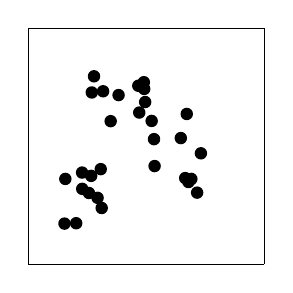
\begin{tikzpicture}[scale=1.5]
			\draw (0,0) -- (2,0);
			\draw (2,0) -- (2,2);
			\draw (2,2) -- (0,2);
			\draw (0,2) -- (0,0);
			
			\fill (0.456,0.778)circle (1.5pt);
			\fill (0.622,0.478)circle (1.5pt);
			\fill (0.457,0.64)circle (1.5pt);
			\fill (0.614,0.807)circle (1.5pt);
			\fill (0.314,0.724)circle (1.5pt);
			\fill (0.533,0.75)circle (1.5pt);
			\fill (0.514,0.605)circle (1.5pt);
			\fill (0.307,0.346)circle (1.5pt);
			\fill (0.406,0.349)circle (1.5pt);
			\fill (0.587,0.564)circle (1.5pt);
			
			\fill (1.065,1.061)circle (1.5pt);
			\fill (1.045,1.215)circle (1.5pt);
			\fill (1.292,1.07)circle (1.5pt);
			\fill (1.381,0.724)circle (1.5pt);
			\fill (1.43,0.608)circle (1.5pt);
			\fill (1.342,1.274)circle (1.5pt);
			\fill (1.329,0.731)circle (1.5pt);
			\fill (1.462,0.941)circle (1.5pt);
			\fill (1.357,0.698)circle (1.5pt);
			\fill (1.07,0.833)circle (1.5pt);
			
			\fill (0.765,1.434)circle (1.5pt);
			\fill (0.557,1.593)circle (1.5pt);
			\fill (0.698,1.213)circle (1.5pt);
			\fill (0.634,1.466)circle (1.5pt);
			\fill (0.979,1.543)circle (1.5pt);
			\fill (0.99,1.375)circle (1.5pt);
			\fill (0.538,1.456)circle (1.5pt);
			\fill (0.932,1.513)circle (1.5pt);
			\fill (0.982,1.486)circle (1.5pt);
			\fill (0.94,1.286)circle (1.5pt);
		\end{tikzpicture}
		\caption*{\footnotesize Original Set}
		\label{fig:badrep}
	\end{minipage}
	\begin{minipage}{0.4\linewidth}
		\centering
		\begin{tikzpicture}[scale=1.5]
		\draw (0,0) -- (2,0);
		\draw (2,0) -- (2,2);
		\draw (2,2) -- (0,2);
		\draw (0,2) -- (0,0);
		
		\fill (0.622,0.478)circle (1.5pt);
		\fill (1.462,0.941)circle (1.5pt);
		\fill (0.765,1.434)circle (1.5pt);
		\end{tikzpicture}		
		\caption*{\footnotesize Representative Set}
		\label{fig:goodrep}
	\end{minipage}
	\label{fig:rep}
\end{figure}
		\item The set of points can change (zooming/panning)
	\end{itemize}
}

\frame{
	\frametitle{Visualisation and Analysis of Geographic Information}
	\framesubtitle{1. Work Plan}
		\begin{itemize}
			\item $1^{st}$ Semester
			\begin{itemize} 
				\item Formalise the representation problem as the $k$-centre problem.
				\item Development of a branch-and-bound approach.
				\item Implement an integer linear programming approach.
				\item Experimental analysis of the algorithms.
			\end{itemize}
		\end{itemize}
		\begin{itemize}
			\item $2^{nd}$ Semester
			\begin{itemize}
				\item Formalise the representation problem as geometric disk cover.
				\item Development of an approximation algorithm approach.
				\item Development of heuristic speed-ups.
				\item Experimental analysis of the algorithms.
			\end{itemize}
		\end{itemize}
}


\frame{
	\frametitle{2. $k$-Centre Problem}	
	\framesubtitle{Defining Coverage}
	\begin{itemize}
		\item Given a set $N$ of points, find a subset $P$ of $k$ centroids.
		\item Goal : to minimise the largest distance between a point and its closest centroid.
	\end{itemize}
	\begin{figure}[H]
	\centering
	\begin{minipage}{0.4\linewidth}
		\centering
		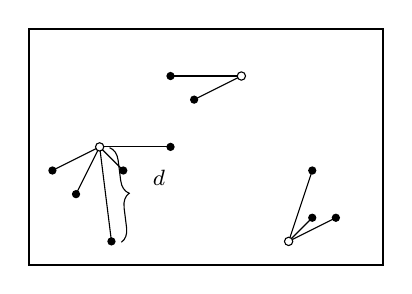
\begin{tikzpicture}[scale=0.3]
		
		\draw [<->,thick] (0,0) rectangle (15,10) {};
		%centroids
		
		%Left Group
%		\fill ( 7,7) circle (5pt);
		\fill ( 1,4) circle (5pt);
		\fill ( 4,4) circle (5pt);
		\fill ( 2,3) circle (5pt);
		\fill (3.5,1) circle (5pt);
		\fill ( 6,5) circle (5pt);
		
		%Middle Group
		
		\fill ( 7,7) circle (5pt);
		\fill ( 6,8) circle (5pt);
		
		%Right Group
		\fill (12,2) circle (5pt);
		\fill (12,4) circle (5pt);
		\fill (13,2) circle (5pt);
		
		%Lines
		\draw [-] (1,4) -- (3,5);
		\draw [-] (4,4) -- (3,5);
		\draw [-] (2,3) -- (3,5);
		\draw [-] (3.5,1) -- (3,5);
		\draw [-] (6,5) -- (3,5);
		
		\draw [-] (7,7) -- (9,8);
		\draw [-] (6,8) -- (9,8);
		
		\draw [-] (12,2) -- (11,1);
		\draw [-] (12,4) -- (11,1);
		\draw [-] (13,2) -- (11,1);
		\fill [white] (11,1) circle (5pt);
		\fill [white] ( 3,5) circle (5pt);
		\fill [white] ( 9,8) circle (5pt);
		
		\draw (11,1) circle (5pt);
		\draw ( 3,5) circle (5pt);
		\draw ( 9,8) circle (5pt);
		
		\draw [decorate,decoration={brace,amplitude=5pt},xshift=12pt,yshift=-1pt]
		(3,5) -- (3.5,1)node [black,midway,xshift=10pt] {\footnotesize$d$};
		\end{tikzpicture}
		\caption*{Non-optimal Assignment}
		\label{fig:badcov}
	\end{minipage}
	\begin{minipage}{0.4\linewidth}
		\centering
		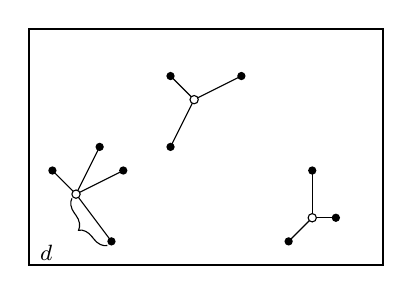
\begin{tikzpicture}[scale=0.3]
		
		\draw [<->,thick] (0,0) rectangle (15,10) {};
		%centroids
		
		%Left Group
		\fill ( 1,4) circle (5pt);
		\fill ( 4,4) circle (5pt);
		\fill ( 3,5) circle (5pt);
		\fill (3.5,1) circle (5pt);
		
		%Middle Group
		\fill ( 6,5) circle (5pt);
		\fill ( 9,8) circle (5pt);
		\fill ( 6,8) circle (5pt);
		
		%Right Group
		\fill (11,1) circle (5pt);
		\fill (12,4) circle (5pt);
		\fill (13,2) circle (5pt);
		
		%\pause
		%Lines
		\draw [-] (1,4) -- (2,3);
		\draw [-] (4,4) -- (2,3);
		\draw [-] (3,5) -- (2,3);
		\draw [-] (3.5,1) -- (2,3);
		
		\draw [-] (6,5) -- (7,7);
		\draw [-] (9,8) -- (7,7);
		\draw [-] (6,8) -- (7,7);
		
		\draw [-] (11,1) -- (12,2);
		\draw [-] (12,4) -- (12,2);
		\draw [-] (13,2) -- (12,2);
		
		\fill [white] ( 2,3) circle (5pt);
		\fill [white] (12,2) circle (5pt);
		\fill [white] ( 7,7) circle (5pt);
		
		\draw ( 2,3) circle (5pt);
		\draw (12,2) circle (5pt);
		\draw ( 7,7) circle (5pt);
		
		%Circles
		%\draw [dashed] (2,3) circle (2.5);
		%\draw [dashed] (7,7) circle (2.236);
		%\draw [dashed] (12,2) circle (2);
		%\pause
		\draw [decorate,decoration={brace,amplitude=5pt},xshift=-5pt,yshift=-5pt]
		(3.5,1) -- (2,3)node [black,midway,xshift=-10pt,yshift=-5pt] {\footnotesize$d$};
		\end{tikzpicture}		
		\caption*{Optimal Assignment}
		\label{fig:goodcov}
	\end{minipage}
	\caption{Different assignments for the same set of points}
	\label{fig:cov}
\end{figure}
	\begin{equation*}
	\min_{\substack{P \subseteq N\\ \lvert P \rvert = k}}{\max_{n \in N}{\min_{p \in P}{\lVert p-n \rVert}}}
	\end{equation*}
}

\frame{
	\frametitle{2. $k$-Centre Problem}	
	\framesubtitle{Branch-and-bound}
	\begin{itemize}
		\item Branching
		\begin{itemize}
			\medskip
			\item Divide search space in a binary tree
			\medskip
			\item At each step, decide if a point is a centroid or non-centroid
			\medskip
			\item Update objective function accordingly
		\end{itemize}
		\item Bound
		\begin{itemize}
			\medskip
			\item Assume best possible case
			\medskip
			\item Prune tree
		\end{itemize}
	\end{itemize}
}

\frame{
	\frametitle{2. $k$-Centre Problem}	
	\framesubtitle{Na\"ive Branch-and-bound}
	\begin{minipage}{0.48\linewidth}
	\begin{itemize}
		\item Inserting a Centroid
		\begin{itemize}
			\medskip
			\item Search all non-centroids for assignment update
			\medskip
			\item Smaller or equal coverage
		\end{itemize}
		\vspace{0.5cm}
		\item Inserting a Non-centroid
		\begin{itemize}
			\medskip
			\item Search for closest centroid
			\medskip
			\item Larger or equal coverage
		\end{itemize}
	\end{itemize}
	\end{minipage}
	\begin{minipage}{0.48\linewidth}
		\vspace{-15pt}
		\input{Figures/npoint}
	\end{minipage}
}
\frame{
	\frametitle{2. $k$-Centre Problem}	
	\framesubtitle{Na\"ive Branch-and-bound}
	\begin{minipage}{0.48\linewidth}
	\begin{itemize}
		\item Removing a Centroid
		\begin{itemize}
			\medskip
			\item Update all non-centroids
			\medskip
			\item Larger or equal coverage
		\end{itemize}
		\vspace{0.5cm}
		\item Removing a Non-centroid
		\begin{itemize}
			\medskip
			\item Update objective function
			\medskip
			\item Smaller or equal coverage
		\end{itemize}
	\end{itemize}
	\end{minipage}
	\begin{minipage}{0.48\linewidth}
		\vspace{-15pt}
		\input{Figures/rpoint}
	\end{minipage}
}

\frame{
	\frametitle{2. $k$-Centre Problem}
	\framesubtitle{Na\"ive Branch-and-bound}
	\begin{itemize}
		\item Assume all remaining points are centroids
		\item If the closest one is too far, the branch can be pruned
	\end{itemize}		
	\begin{figure}[!h]
\centering
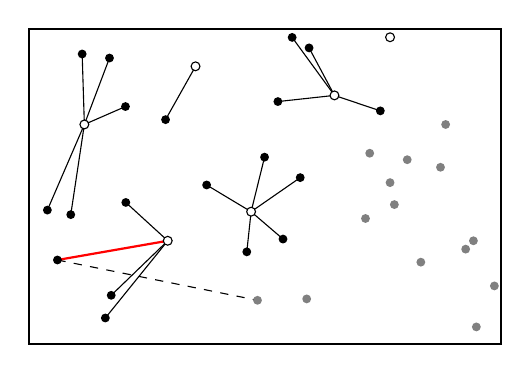
\begin{tikzpicture}[scale=0.4]
\draw [<->,thick] (0,0) rectangle (15,10) {};
\draw [-,dashed](0.909705882352941, 2.659076923076923) -- (7.261764705882353, 1.3796923076923076);
\fill [gray](7.261764705882353, 1.3796923076923076)circle(4pt);
\fill [gray](10.690588235294118, 3.9763076923076923)circle(4pt);
\draw [-](3.0697058823529413, 7.531076923076923) -- (1.7647058823529411, 6.961538461538462);
\fill(3.0697058823529413, 7.531076923076923)circle(4pt);
\draw [-](11.161764705882353, 7.393538461538461) -- (9.705882352941176, 7.884615384615385);
\fill(11.161764705882353, 7.393538461538461)circle(4pt);
\draw [-](2.4308823529411763, 0.8175384615384615) -- (4.411764705882353, 3.269230769230769);
\fill(2.4308823529411763, 0.8175384615384615)circle(4pt);
\fill [gray](11.60735294117647, 4.418461538461538)circle(4pt);
\draw [-](2.617058823529412, 1.5375384615384617) -- (4.411764705882353, 3.269230769230769);
\fill(2.617058823529412, 1.5375384615384617)circle(4pt);
\draw [-](8.617941176470588, 5.274153846153846) -- (7.0588235294117645, 4.1923076923076925);
\fill(8.617941176470588, 5.274153846153846)circle(4pt);
\draw [-](0.5902941176470589, 4.243076923076923) -- (1.7647058823529411, 6.961538461538462);
\fill(0.5902941176470589, 4.243076923076923)circle(4pt);
\draw [-](1.695, 9.199076923076923) -- (1.7647058823529411, 6.961538461538462);
\fill(1.695, 9.199076923076923)circle(4pt);
\draw [-](4.342941176470588, 7.114769230769231) -- (5.294117647058823, 8.807692307692308);
\fill(4.342941176470588, 7.114769230769231)circle(4pt);
\draw [-](8.899411764705881, 9.392923076923077) -- (9.705882352941176, 7.884615384615385);
\fill(8.899411764705881, 9.392923076923077)circle(4pt);
\draw [-](7.485882352941177, 5.924) -- (7.0588235294117645, 4.1923076923076925);
\fill(7.485882352941177, 5.924)circle(4pt);
\fill [gray](14.21029411764706, 0.5341538461538462)circle(4pt);
\fill [gray](14.78294117647059, 1.8356923076923077)circle(4pt);
\fill [gray](13.871470588235294, 3.0033846153846158)circle(4pt);
\draw [-](1.333235294117647, 4.099076923076923) -- (1.7647058823529411, 6.961538461538462);
\fill(1.333235294117647, 4.099076923076923)circle(4pt);
\draw [-](2.5623529411764707, 9.070769230769232) -- (1.7647058823529411, 6.961538461538462);
\fill(2.5623529411764707, 9.070769230769232)circle(4pt);
\fill [gray](12.015882352941176, 5.842769230769231)circle(4pt);
\fill [gray](12.448235294117648, 2.5898461538461537)circle(4pt);
\draw [-,thick,red](0.909705882352941, 2.659076923076923) -- (4.411764705882353, 3.269230769230769);
\fill(0.909705882352941, 2.659076923076923)circle(4pt);
\draw [-](3.0811764705882356, 4.485846153846154) -- (4.411764705882353, 3.269230769230769);
\fill(3.0811764705882356, 4.485846153846154)circle(4pt);
\draw [-](8.362058823529411, 9.726153846153846) -- (9.705882352941176, 7.884615384615385);
\fill(8.362058823529411, 9.726153846153846)circle(4pt);
\fill [gray](10.824705882352943, 6.048615384615385)circle(4pt);
\draw [-](5.647058823529412, 5.040615384615384) -- (7.0588235294117645, 4.1923076923076925);
\fill(5.647058823529412, 5.040615384615384)circle(4pt);
\draw [-](8.071764705882353, 3.3236923076923075) -- (7.0588235294117645, 4.1923076923076925);
\fill(8.071764705882353, 3.3236923076923075)circle(4pt);
\fill [gray](13.072058823529412, 5.602769230769231)circle(4pt);
\draw [-](6.922058823529412, 2.917538461538462) -- (7.0588235294117645, 4.1923076923076925);
\fill(6.922058823529412, 2.917538461538462)circle(4pt);
\draw [-](7.909411764705883, 7.688923076923077) -- (9.705882352941176, 7.884615384615385);
\fill(7.909411764705883, 7.688923076923077)circle(4pt);
\fill [gray](8.823529411764707, 1.4230769230769231)circle(4pt);
\fill [gray](11.470588235294118, 5.115384615384615)circle(4pt);
\fill [gray](13.235294117647058, 6.961538461538462)circle(4pt);
\fill [gray](14.117647058823529, 3.269230769230769)circle(4pt);
\fill [white](1.7647058823529411, 6.961538461538462)circle(4pt);
\draw [black](1.7647058823529411, 6.961538461538462)circle(4pt);
\fill [white](4.411764705882353, 3.269230769230769)circle(4pt);
\draw [black](4.411764705882353, 3.269230769230769)circle(4pt);
\fill [white](5.294117647058823, 8.807692307692308)circle(4pt);
\draw [black](5.294117647058823, 8.807692307692308)circle(4pt);
\fill [white](9.705882352941176, 7.884615384615385)circle(4pt);
\draw [black](9.705882352941176, 7.884615384615385)circle(4pt);
\fill [white](11.470588235294118, 9.73076923076923)circle(4pt);
\draw [black](11.470588235294118, 9.73076923076923)circle(4pt);
\fill [white](7.0588235294117645, 4.1923076923076925)circle(4pt);
\draw [black](7.0588235294117645, 4.1923076923076925)circle(4pt);
\end{tikzpicture}
\caption[Illustration of the lower bound calculation.]{Illustration of the lower bound calculation. The dashed line represents the distance in the lower bound. Since the value is larger than the current objective function, in red, if there has been found a branch with a better solution, then the current branch is pruned.}
\label{fig:bound}
\end{figure}

	\begin{itemize}
		\item Only if a better solution has been found
	\end{itemize}		
}

\frame{
	\frametitle{2. $k$-Centre Problem}	
	\framesubtitle{Geometric Branch-and-bound}	
	\begin{itemize}
		\item Use geometric structures to speed-up the update of the objective function
		\item Delaunay triangulations
		\item Sort points by Hilbert curve
	\end{itemize}
	\input{Figures/dt1}
}


\frame{
	\frametitle{2. $k$-Centre Problem}	
	\framesubtitle{Geometric Branch-and-bound}	
	\begin{minipage}{0.6\linewidth}
	\begin{itemize}
		\item Inserting a Centroid
		\begin{itemize}
			\medskip
			\item Insert centroid in triangulation
			\medskip
			\item Search all non-centroids for assignment update
			\medskip
			\item Smaller or equal coverage
		\end{itemize}
		\vspace{0.5cm}
		\item Inserting a Non-centroid
		\begin{itemize}
			\medskip
			\item Search for closest centroid using greedy routing
			\medskip
			\item Update objective function
			\medskip
			\item Larger or equal coverage
		\end{itemize}
	\end{itemize}
	\end{minipage}
	\begin{minipage}{0.38\linewidth}
		\input{Figures/gnpoint}
	\end{minipage}
}


\frame{
	\frametitle{2. $k$-Centre Problem}	
	\framesubtitle{Na\"ive Branch-and-bound}
	\begin{minipage}{0.6\linewidth}
		\begin{itemize}
			\item Removing a Centroid
			\begin{itemize}
				\medskip
				\item Revert assignment
				\medskip
				\item Remove centroid from triangulation
				\medskip
				\item Larger or equal coverage 
			\end{itemize}
			\vspace{0.5cm}
			\item Removing a Non-centroid
			\begin{itemize}
				\medskip
				\item Update objective function
				\medskip
				\item Revert assignment
				\medskip
				\item Smaller or equal coverage 
			\end{itemize}
		\end{itemize}
	\end{minipage}
	\begin{minipage}{0.38\linewidth}
		\input{Figures/grpoint}
	\end{minipage}
}

\frame{
	\frametitle{2. $k$-Centre Problem}	
	\framesubtitle{Algorithm Comparison - Effect of N}
	\begin{figure}[H] 
	\begin{subfigure}[b]{0.5\linewidth}
		\centering
		\includegraphics[width=0.9\linewidth]{Pictures/k1} 
		\caption{$K=0.25N$} 
		\label{fig:fixed_k:a} 
	\end{subfigure}%% 
	\begin{subfigure}[b]{0.5\linewidth}
		\centering
		\includegraphics[width=0.9\linewidth]{Pictures/k2} 
		\caption{$K=0.5N$} 
		\label{fig:fixed_k:b} 
	\end{subfigure} 
	\begin{center}
	\begin{subfigure}[b]{0.5\linewidth}
		\includegraphics[width=0.9\linewidth]{Pictures/k3} 
		\caption{$K=0.75N$} 
		\label{fig:fixed_k:c} 
	\end{subfigure}
	\end{center}
	\begin{center}
    \textcolor{blue}{\cmark}\ -- Integer Linear Programming\quad   \textcolor{red}{\tmark}\ -- Delaunay Assisted B\&B\quad \textcolor{OliveGreen}{\smark}\ -- Naive B\&B
    \end{center}
	\caption{CPU-time for different values of $K$ with varying values of $N$}
	\label{fig:fixed_k} 
\end{figure}

		
}
\frame{
	\frametitle{2. $k$-Centre Problem}	
	\framesubtitle{Algorithm Comparison - Effect of K}
	\begin{figure}[t] 
  \begin{subfigure}[b]{0.3\linewidth}
    \centering
    \includegraphics[width=0.9\linewidth]{Pictures/n10} 
    \caption{$N=10$} 
    \label{fig:fixed_n:a} 
  \end{subfigure}%% 
  \begin{subfigure}[b]{0.3\linewidth}
    \centering
    \includegraphics[width=0.9\linewidth]{Pictures/n20} 
    \caption{$N=20$} 
    \label{fig:fixed_n:b} 
  \end{subfigure} 
  \begin{subfigure}[b]{0.3\linewidth}
    \centering
    \includegraphics[width=0.9\linewidth]{Pictures/n30} 
    \caption{$N=30$} 
    \label{fig:fixed_n:c} 
  \end{subfigure}%%
  \begin{subfigure}[b]{0.3\linewidth}
    \centering
    \includegraphics[width=0.9\linewidth]{Pictures/n40} 
    \caption{$N=40$} 
    \label{fig:fixed_n:d} 
  \end{subfigure} 
  \vspace{2ex}
  \begin{center}
  \footnotesize
  \textcolor{blue}{\cmark}\ -- Integer Linear Programming \textcolor{red}{\tmark}\ -- Delaunay Assisted B\&B \textcolor{green}{\smark}\ -- Naive B\&B
  \end{center}
  %\caption{CPU-time for different values of $N$ with varying $K$}
  %\label{fig:fixed_n} 
\end{figure}

		
}

\frame{
	\frametitle{2. $k$-Centre Problem}	
	\framesubtitle{Disadvantages}
	\begin{itemize}
		\item All approaches are too slow.
		\medskip
		\item So solve the problem we need to know how many clusters to choose.
		\medskip
	\end{itemize}
	\centering
	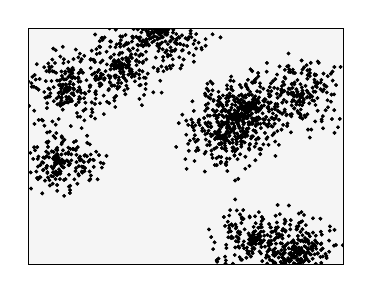
\begin{tikzpicture}
		\fill[lightgray!15,draw=black] (0,0) rectangle (4,3);
		\clip(0,0) rectangle (4,3);
		\fill (3.324,2.228) circle (0.7pt);
\fill (3.109,2.329) circle (0.7pt);
\fill (3.500,2.101) circle (0.7pt);
\fill (3.675,2.297) circle (0.7pt);
\fill (3.252,2.285) circle (0.7pt);
\fill (3.745,1.729) circle (0.7pt);
\fill (3.909,2.278) circle (0.7pt);
\fill (3.428,1.924) circle (0.7pt);
\fill (3.222,2.265) circle (0.7pt);
\fill (3.470,2.430) circle (0.7pt);
\fill (3.934,1.743) circle (0.7pt);
\fill (3.058,2.163) circle (0.7pt);
\fill (3.280,2.065) circle (0.7pt);
\fill (3.852,2.157) circle (0.7pt);
\fill (2.753,1.943) circle (0.7pt);
\fill (3.365,2.433) circle (0.7pt);
\fill (3.288,1.759) circle (0.7pt);
\fill (3.760,2.281) circle (0.7pt);
\fill (3.539,2.208) circle (0.7pt);
\fill (3.522,2.268) circle (0.7pt);
\fill (3.535,2.530) circle (0.7pt);
\fill (3.648,2.025) circle (0.7pt);
\fill (3.635,2.346) circle (0.7pt);
\fill (3.312,2.444) circle (0.7pt);
\fill (3.545,2.358) circle (0.7pt);
\fill (3.801,2.085) circle (0.7pt);
\fill (3.455,2.140) circle (0.7pt);
\fill (3.031,2.559) circle (0.7pt);
\fill (3.455,2.147) circle (0.7pt);
\fill (3.726,1.843) circle (0.7pt);
\fill (3.383,2.310) circle (0.7pt);
\fill (3.496,2.082) circle (0.7pt);
\fill (3.885,2.160) circle (0.7pt);
\fill (3.091,1.863) circle (0.7pt);
\fill (3.457,2.290) circle (0.7pt);
\fill (3.328,1.904) circle (0.7pt);
\fill (3.605,2.133) circle (0.7pt);
\fill (3.677,2.578) circle (0.7pt);
\fill (3.406,2.030) circle (0.7pt);
\fill (3.445,2.028) circle (0.7pt);
\fill (3.588,2.560) circle (0.7pt);
\fill (3.244,2.200) circle (0.7pt);
\fill (3.867,2.335) circle (0.7pt);
\fill (3.072,2.138) circle (0.7pt);
\fill (3.727,1.818) circle (0.7pt);
\fill (3.496,2.056) circle (0.7pt);
\fill (3.638,2.311) circle (0.7pt);
\fill (3.349,2.069) circle (0.7pt);
\fill (3.355,2.243) circle (0.7pt);
\fill (3.477,2.147) circle (0.7pt);
\fill (2.922,2.387) circle (0.7pt);
\fill (3.376,2.130) circle (0.7pt);
\fill (3.673,2.113) circle (0.7pt);
\fill (3.385,2.147) circle (0.7pt);
\fill (3.455,1.868) circle (0.7pt);
\fill (3.611,2.245) circle (0.7pt);
\fill (3.336,1.678) circle (0.7pt);
\fill (3.548,2.128) circle (0.7pt);
\fill (3.777,1.958) circle (0.7pt);
\fill (3.346,2.020) circle (0.7pt);
\fill (3.419,2.342) circle (0.7pt);
\fill (3.474,2.128) circle (0.7pt);
\fill (3.226,2.055) circle (0.7pt);
\fill (3.807,1.997) circle (0.7pt);
\fill (3.545,1.907) circle (0.7pt);
\fill (2.962,2.011) circle (0.7pt);
\fill (3.308,2.233) circle (0.7pt);
\fill (3.723,2.344) circle (0.7pt);
\fill (3.456,1.907) circle (0.7pt);
\fill (3.844,2.422) circle (0.7pt);
\fill (3.627,2.195) circle (0.7pt);
\fill (3.168,2.233) circle (0.7pt);
\fill (3.406,2.225) circle (0.7pt);
\fill (3.864,2.449) circle (0.7pt);
\fill (3.346,2.294) circle (0.7pt);
\fill (3.803,2.391) circle (0.7pt);
\fill (3.483,2.208) circle (0.7pt);
\fill (3.503,2.504) circle (0.7pt);
\fill (3.595,1.713) circle (0.7pt);
\fill (3.461,1.968) circle (0.7pt);
\fill (3.306,2.679) circle (0.7pt);
\fill (3.164,2.036) circle (0.7pt);
\fill (3.494,2.169) circle (0.7pt);
\fill (3.469,2.164) circle (0.7pt);
\fill (3.472,2.151) circle (0.7pt);
\fill (3.957,1.848) circle (0.7pt);
\fill (3.644,1.816) circle (0.7pt);
\fill (3.361,2.474) circle (0.7pt);
\fill (3.647,2.194) circle (0.7pt);
\fill (3.424,2.152) circle (0.7pt);
\fill (3.472,2.146) circle (0.7pt);
\fill (3.522,1.873) circle (0.7pt);
\fill (3.217,2.174) circle (0.7pt);
\fill (3.639,2.402) circle (0.7pt);
\fill (2.914,2.089) circle (0.7pt);
\fill (3.689,2.560) circle (0.7pt);
\fill (3.237,1.772) circle (0.7pt);
\fill (3.574,2.473) circle (0.7pt);
\fill (3.967,2.508) circle (0.7pt);
\fill (3.451,2.155) circle (0.7pt);
\fill (3.739,2.200) circle (0.7pt);
\fill (3.348,1.910) circle (0.7pt);
\fill (3.360,2.088) circle (0.7pt);
\fill (3.075,2.146) circle (0.7pt);
\fill (3.460,2.158) circle (0.7pt);
\fill (3.294,2.185) circle (0.7pt);
\fill (3.472,2.590) circle (0.7pt);
\fill (3.576,1.612) circle (0.7pt);
\fill (3.259,2.471) circle (0.7pt);
\fill (3.386,2.431) circle (0.7pt);
\fill (3.787,2.260) circle (0.7pt);
\fill (3.082,2.300) circle (0.7pt);
\fill (3.441,1.920) circle (0.7pt);
\fill (3.538,2.120) circle (0.7pt);
\fill (3.376,1.979) circle (0.7pt);
\fill (3.412,2.132) circle (0.7pt);
\fill (2.866,2.048) circle (0.7pt);
\fill (3.569,2.046) circle (0.7pt);
\fill (3.509,1.891) circle (0.7pt);
\fill (3.857,1.847) circle (0.7pt);
\fill (3.256,1.940) circle (0.7pt);
\fill (3.167,2.117) circle (0.7pt);
\fill (3.468,2.163) circle (0.7pt);
\fill (3.440,2.087) circle (0.7pt);
\fill (3.478,2.021) circle (0.7pt);
\fill (3.458,2.117) circle (0.7pt);
\fill (3.353,2.155) circle (0.7pt);
\fill (3.547,2.465) circle (0.7pt);
\fill (3.792,2.184) circle (0.7pt);
\fill (3.283,1.905) circle (0.7pt);
\fill (3.059,1.967) circle (0.7pt);
\fill (3.632,2.078) circle (0.7pt);
\fill (3.376,2.079) circle (0.7pt);
\fill (3.668,2.315) circle (0.7pt);
\fill (3.332,2.445) circle (0.7pt);
\fill (3.013,2.094) circle (0.7pt);
\fill (3.439,2.074) circle (0.7pt);
\fill (3.122,1.841) circle (0.7pt);
\fill (3.417,2.159) circle (0.7pt);
\fill (3.764,2.273) circle (0.7pt);
\fill (3.315,2.477) circle (0.7pt);
\fill (3.346,2.183) circle (0.7pt);
\fill (3.581,2.156) circle (0.7pt);
\fill (3.484,1.851) circle (0.7pt);
\fill (3.625,2.195) circle (0.7pt);
\fill (3.303,2.164) circle (0.7pt);
\fill (2.858,1.985) circle (0.7pt);
\fill (3.346,2.290) circle (0.7pt);
\fill (3.068,2.252) circle (0.7pt);
\fill (3.289,2.515) circle (0.7pt);
\fill (3.844,2.067) circle (0.7pt);
\fill (3.419,2.194) circle (0.7pt);
\fill (3.887,1.960) circle (0.7pt);
\fill (3.484,2.476) circle (0.7pt);
\fill (3.306,2.522) circle (0.7pt);
\fill (3.329,2.171) circle (0.7pt);
\fill (3.381,1.984) circle (0.7pt);
\fill (3.483,2.153) circle (0.7pt);
\fill (3.408,2.057) circle (0.7pt);
\fill (3.380,2.287) circle (0.7pt);
\fill (3.750,2.424) circle (0.7pt);
\fill (3.665,2.253) circle (0.7pt);
\fill (3.742,1.884) circle (0.7pt);
\fill (3.553,1.712) circle (0.7pt);
\fill (3.495,2.054) circle (0.7pt);
\fill (3.417,2.192) circle (0.7pt);
\fill (3.888,2.508) circle (0.7pt);
\fill (3.676,1.952) circle (0.7pt);
\fill (3.040,1.990) circle (0.7pt);
\fill (3.252,2.206) circle (0.7pt);
\fill (3.265,2.361) circle (0.7pt);
\fill (3.576,2.393) circle (0.7pt);
\fill (3.713,2.225) circle (0.7pt);
\fill (3.651,2.266) circle (0.7pt);
\fill (3.578,2.119) circle (0.7pt);
\fill (3.094,1.969) circle (0.7pt);
\fill (2.896,1.960) circle (0.7pt);
\fill (3.172,1.950) circle (0.7pt);
\fill (3.714,2.310) circle (0.7pt);
\fill (3.227,2.190) circle (0.7pt);
\fill (3.216,1.712) circle (0.7pt);
\fill (3.420,1.949) circle (0.7pt);
\fill (3.484,2.160) circle (0.7pt);
\fill (3.059,2.044) circle (0.7pt);
\fill (3.672,2.297) circle (0.7pt);
\fill (3.577,2.431) circle (0.7pt);
\fill (3.639,2.415) circle (0.7pt);
\fill (3.550,2.404) circle (0.7pt);
\fill (2.845,2.455) circle (0.7pt);
\fill (3.607,2.086) circle (0.7pt);
\fill (3.458,2.124) circle (0.7pt);
\fill (3.754,2.223) circle (0.7pt);
\fill (3.553,2.181) circle (0.7pt);
\fill (3.368,2.179) circle (0.7pt);
\fill (3.547,2.193) circle (0.7pt);
\fill (3.459,2.065) circle (0.7pt);
\fill (3.890,1.671) circle (0.7pt);
\fill (3.475,2.248) circle (0.7pt);
\fill (3.656,2.408) circle (0.7pt);
\fill (3.341,1.881) circle (0.7pt);
\fill (2.573,0.421) circle (0.7pt);
\fill (2.594,0.492) circle (0.7pt);
\fill (2.873,0.199) circle (0.7pt);
\fill (2.778,0.215) circle (0.7pt);
\fill (2.840,0.168) circle (0.7pt);
\fill (3.158,0.533) circle (0.7pt);
\fill (2.742,0.206) circle (0.7pt);
\fill (3.167,0.755) circle (0.7pt);
\fill (2.862,0.477) circle (0.7pt);
\fill (2.514,0.250) circle (0.7pt);
\fill (2.866,0.273) circle (0.7pt);
\fill (3.368,0.102) circle (0.7pt);
\fill (3.145,0.467) circle (0.7pt);
\fill (2.812,0.611) circle (0.7pt);
\fill (2.802,0.131) circle (0.7pt);
\fill (2.933,0.266) circle (0.7pt);
\fill (2.734,0.579) circle (0.7pt);
\fill (2.866,0.416) circle (0.7pt);
\fill (3.147,0.264) circle (0.7pt);
\fill (3.267,0.430) circle (0.7pt);
\fill (3.142,0.618) circle (0.7pt);
\fill (2.966,0.475) circle (0.7pt);
\fill (2.599,0.011) circle (0.7pt);
\fill (2.956,0.139) circle (0.7pt);
\fill (2.663,0.403) circle (0.7pt);
\fill (2.778,0.177) circle (0.7pt);
\fill (3.076,0.356) circle (0.7pt);
\fill (2.881,0.611) circle (0.7pt);
\fill (2.700,0.062) circle (0.7pt);
\fill (2.823,0.304) circle (0.7pt);
\fill (3.060,0.187) circle (0.7pt);
\fill (3.252,0.069) circle (0.7pt);
\fill (3.410,0.481) circle (0.7pt);
\fill (2.936,0.384) circle (0.7pt);
\fill (3.248,0.219) circle (0.7pt);
\fill (2.899,0.339) circle (0.7pt);
\fill (3.202,0.364) circle (0.7pt);
\fill (2.887,0.320) circle (0.7pt);
\fill (2.867,0.410) circle (0.7pt);
\fill (3.108,0.180) circle (0.7pt);
\fill (3.359,0.110) circle (0.7pt);
\fill (2.888,0.524) circle (0.7pt);
\fill (2.878,0.333) circle (0.7pt);
\fill (2.399,0.035) circle (0.7pt);
\fill (2.880,0.337) circle (0.7pt);
\fill (2.728,0.246) circle (0.7pt);
\fill (2.667,0.290) circle (0.7pt);
\fill (3.036,0.012) circle (0.7pt);
\fill (2.866,0.377) circle (0.7pt);
\fill (2.909,0.315) circle (0.7pt);
\fill (2.323,0.348) circle (0.7pt);
\fill (2.553,0.461) circle (0.7pt);
\fill (2.942,0.317) circle (0.7pt);
\fill (3.433,0.488) circle (0.7pt);
\fill (2.690,0.636) circle (0.7pt);
\fill (2.956,0.418) circle (0.7pt);
\fill (2.987,0.418) circle (0.7pt);
\fill (3.318,0.133) circle (0.7pt);
\fill (3.145,0.126) circle (0.7pt);
\fill (3.301,0.080) circle (0.7pt);
\fill (3.047,0.275) circle (0.7pt);
\fill (2.718,0.244) circle (0.7pt);
\fill (2.950,0.263) circle (0.7pt);
\fill (2.367,0.281) circle (0.7pt);
\fill (2.901,0.306) circle (0.7pt);
\fill (3.124,0.312) circle (0.7pt);
\fill (2.748,0.445) circle (0.7pt);
\fill (2.859,0.299) circle (0.7pt);
\fill (2.797,0.266) circle (0.7pt);
\fill (2.832,0.249) circle (0.7pt);
\fill (2.858,0.401) circle (0.7pt);
\fill (3.116,0.158) circle (0.7pt);
\fill (3.128,0.109) circle (0.7pt);
\fill (3.235,0.124) circle (0.7pt);
\fill (2.887,0.307) circle (0.7pt);
\fill (2.636,0.457) circle (0.7pt);
\fill (2.853,0.294) circle (0.7pt);
\fill (2.417,0.075) circle (0.7pt);
\fill (2.786,0.142) circle (0.7pt);
\fill (2.826,0.340) circle (0.7pt);
\fill (2.506,0.011) circle (0.7pt);
\fill (2.805,0.316) circle (0.7pt);
\fill (2.646,0.354) circle (0.7pt);
\fill (3.083,0.469) circle (0.7pt);
\fill (2.828,0.100) circle (0.7pt);
\fill (2.830,0.293) circle (0.7pt);
\fill (3.310,0.749) circle (0.7pt);
\fill (2.830,0.332) circle (0.7pt);
\fill (2.813,0.597) circle (0.7pt);
\fill (2.950,0.475) circle (0.7pt);
\fill (2.632,0.508) circle (0.7pt);
\fill (2.812,0.262) circle (0.7pt);
\fill (2.598,0.338) circle (0.7pt);
\fill (3.347,0.196) circle (0.7pt);
\fill (2.801,0.162) circle (0.7pt);
\fill (3.326,0.504) circle (0.7pt);
\fill (2.714,0.059) circle (0.7pt);
\fill (2.679,0.213) circle (0.7pt);
\fill (3.274,0.248) circle (0.7pt);
\fill (3.556,0.205) circle (0.7pt);
\fill (3.087,0.411) circle (0.7pt);
\fill (2.577,0.335) circle (0.7pt);
\fill (3.526,0.499) circle (0.7pt);
\fill (3.215,0.180) circle (0.7pt);
\fill (2.673,0.324) circle (0.7pt);
\fill (2.922,0.350) circle (0.7pt);
\fill (2.623,0.120) circle (0.7pt);
\fill (3.159,0.386) circle (0.7pt);
\fill (2.712,0.598) circle (0.7pt);
\fill (2.553,0.621) circle (0.7pt);
\fill (3.215,0.369) circle (0.7pt);
\fill (3.335,0.564) circle (0.7pt);
\fill (2.810,0.369) circle (0.7pt);
\fill (2.348,0.195) circle (0.7pt);
\fill (3.087,0.301) circle (0.7pt);
\fill (2.553,0.495) circle (0.7pt);
\fill (2.798,0.394) circle (0.7pt);
\fill (3.056,0.097) circle (0.7pt);
\fill (2.534,0.543) circle (0.7pt);
\fill (2.730,0.690) circle (0.7pt);
\fill (2.845,0.367) circle (0.7pt);
\fill (2.770,0.085) circle (0.7pt);
\fill (3.060,0.275) circle (0.7pt);
\fill (3.076,0.472) circle (0.7pt);
\fill (2.884,0.423) circle (0.7pt);
\fill (2.898,0.336) circle (0.7pt);
\fill (2.628,0.826) circle (0.7pt);
\fill (3.225,0.371) circle (0.7pt);
\fill (2.564,0.690) circle (0.7pt);
\fill (2.500,0.489) circle (0.7pt);
\fill (3.460,0.025) circle (0.7pt);
\fill (2.847,0.201) circle (0.7pt);
\fill (3.471,0.666) circle (0.7pt);
\fill (2.669,0.228) circle (0.7pt);
\fill (3.139,0.425) circle (0.7pt);
\fill (2.686,0.092) circle (0.7pt);
\fill (2.950,0.357) circle (0.7pt);
\fill (3.257,0.570) circle (0.7pt);
\fill (2.707,0.526) circle (0.7pt);
\fill (2.918,0.379) circle (0.7pt);
\fill (2.581,0.510) circle (0.7pt);
\fill (2.667,0.341) circle (0.7pt);
\fill (3.101,0.047) circle (0.7pt);
\fill (3.108,0.415) circle (0.7pt);
\fill (3.255,0.519) circle (0.7pt);
\fill (3.436,0.646) circle (0.7pt);
\fill (3.224,0.265) circle (0.7pt);
\fill (2.892,0.295) circle (0.7pt);
\fill (2.968,0.280) circle (0.7pt);
\fill (3.416,0.265) circle (0.7pt);
\fill (2.994,0.308) circle (0.7pt);
\fill (2.543,0.409) circle (0.7pt);
\fill (2.964,0.550) circle (0.7pt);
\fill (2.895,0.322) circle (0.7pt);
\fill (3.204,0.270) circle (0.7pt);
\fill (3.064,0.199) circle (0.7pt);
\fill (2.669,0.418) circle (0.7pt);
\fill (2.540,0.345) circle (0.7pt);
\fill (3.243,0.147) circle (0.7pt);
\fill (2.500,0.099) circle (0.7pt);
\fill (2.967,0.603) circle (0.7pt);
\fill (3.059,0.297) circle (0.7pt);
\fill (2.510,0.052) circle (0.7pt);
\fill (2.688,0.382) circle (0.7pt);
\fill (2.581,0.354) circle (0.7pt);
\fill (2.517,0.208) circle (0.7pt);
\fill (2.738,0.292) circle (0.7pt);
\fill (2.718,0.587) circle (0.7pt);
\fill (2.485,0.603) circle (0.7pt);
\fill (2.828,0.317) circle (0.7pt);
\fill (2.649,0.686) circle (0.7pt);
\fill (2.629,0.216) circle (0.7pt);
\fill (2.638,0.295) circle (0.7pt);
\fill (2.985,0.575) circle (0.7pt);
\fill (3.237,0.451) circle (0.7pt);
\fill (2.955,0.510) circle (0.7pt);
\fill (3.140,0.332) circle (0.7pt);
\fill (2.854,0.335) circle (0.7pt);
\fill (2.922,0.465) circle (0.7pt);
\fill (2.393,0.055) circle (0.7pt);
\fill (2.565,0.422) circle (0.7pt);
\fill (2.884,0.325) circle (0.7pt);
\fill (2.933,0.387) circle (0.7pt);
\fill (3.268,0.548) circle (0.7pt);
\fill (3.171,0.473) circle (0.7pt);
\fill (2.693,0.409) circle (0.7pt);
\fill (3.020,0.087) circle (0.7pt);
\fill (3.110,0.123) circle (0.7pt);
\fill (3.059,0.514) circle (0.7pt);
\fill (2.889,0.334) circle (0.7pt);
\fill (2.955,0.298) circle (0.7pt);
\fill (2.929,0.664) circle (0.7pt);
\fill (2.890,0.257) circle (0.7pt);
\fill (2.902,0.307) circle (0.7pt);
\fill (2.902,0.306) circle (0.7pt);
\fill (2.643,0.476) circle (0.7pt);
\fill (2.810,0.317) circle (0.7pt);
\fill (2.716,0.577) circle (0.7pt);
\fill (2.295,0.444) circle (0.7pt);
\fill (2.862,0.214) circle (0.7pt);
\fill (0.912,2.047) circle (0.7pt);
\fill (1.387,2.789) circle (0.7pt);
\fill (1.154,2.522) circle (0.7pt);
\fill (1.171,2.523) circle (0.7pt);
\fill (1.797,2.520) circle (0.7pt);
\fill (1.271,2.527) circle (0.7pt);
\fill (1.110,2.521) circle (0.7pt);
\fill (0.970,2.883) circle (0.7pt);
\fill (1.677,2.333) circle (0.7pt);
\fill (0.918,2.565) circle (0.7pt);
\fill (1.195,2.615) circle (0.7pt);
\fill (0.904,2.297) circle (0.7pt);
\fill (1.123,2.795) circle (0.7pt);
\fill (1.220,2.210) circle (0.7pt);
\fill (1.647,2.481) circle (0.7pt);
\fill (1.083,2.580) circle (0.7pt);
\fill (1.247,2.328) circle (0.7pt);
\fill (1.096,2.518) circle (0.7pt);
\fill (1.694,2.182) circle (0.7pt);
\fill (0.564,2.496) circle (0.7pt);
\fill (1.496,2.701) circle (0.7pt);
\fill (1.025,2.227) circle (0.7pt);
\fill (1.211,2.411) circle (0.7pt);
\fill (1.461,2.577) circle (0.7pt);
\fill (1.176,2.432) circle (0.7pt);
\fill (0.663,2.576) circle (0.7pt);
\fill (0.847,2.570) circle (0.7pt);
\fill (0.879,2.445) circle (0.7pt);
\fill (1.220,2.541) circle (0.7pt);
\fill (1.424,2.884) circle (0.7pt);
\fill (1.037,2.367) circle (0.7pt);
\fill (1.169,2.766) circle (0.7pt);
\fill (1.098,2.514) circle (0.7pt);
\fill (1.262,2.234) circle (0.7pt);
\fill (0.796,2.607) circle (0.7pt);
\fill (1.409,2.412) circle (0.7pt);
\fill (1.280,2.582) circle (0.7pt);
\fill (1.297,2.642) circle (0.7pt);
\fill (1.159,2.256) circle (0.7pt);
\fill (1.413,2.102) circle (0.7pt);
\fill (1.133,2.232) circle (0.7pt);
\fill (1.199,2.509) circle (0.7pt);
\fill (1.323,2.420) circle (0.7pt);
\fill (1.493,2.292) circle (0.7pt);
\fill (1.245,2.524) circle (0.7pt);
\fill (1.118,2.573) circle (0.7pt);
\fill (1.411,2.274) circle (0.7pt);
\fill (1.202,2.382) circle (0.7pt);
\fill (1.412,2.466) circle (0.7pt);
\fill (0.943,2.875) circle (0.7pt);
\fill (1.158,2.518) circle (0.7pt);
\fill (1.469,2.372) circle (0.7pt);
\fill (1.351,2.391) circle (0.7pt);
\fill (0.859,2.380) circle (0.7pt);
\fill (1.164,2.452) circle (0.7pt);
\fill (1.210,2.446) circle (0.7pt);
\fill (1.271,2.410) circle (0.7pt);
\fill (1.040,2.306) circle (0.7pt);
\fill (0.773,2.200) circle (0.7pt);
\fill (1.151,2.570) circle (0.7pt);
\fill (0.944,2.589) circle (0.7pt);
\fill (1.035,2.317) circle (0.7pt);
\fill (1.154,2.515) circle (0.7pt);
\fill (1.105,2.546) circle (0.7pt);
\fill (1.234,2.161) circle (0.7pt);
\fill (1.718,2.453) circle (0.7pt);
\fill (1.123,2.529) circle (0.7pt);
\fill (1.072,2.272) circle (0.7pt);
\fill (0.908,2.836) circle (0.7pt);
\fill (0.931,2.877) circle (0.7pt);
\fill (0.575,2.608) circle (0.7pt);
\fill (0.897,2.469) circle (0.7pt);
\fill (1.428,2.279) circle (0.7pt);
\fill (0.838,2.593) circle (0.7pt);
\fill (1.282,2.536) circle (0.7pt);
\fill (1.154,2.580) circle (0.7pt);
\fill (0.510,2.572) circle (0.7pt);
\fill (1.369,2.429) circle (0.7pt);
\fill (1.285,2.490) circle (0.7pt);
\fill (1.151,2.342) circle (0.7pt);
\fill (0.656,2.678) circle (0.7pt);
\fill (1.171,2.799) circle (0.7pt);
\fill (0.824,2.600) circle (0.7pt);
\fill (0.857,2.342) circle (0.7pt);
\fill (1.218,2.368) circle (0.7pt);
\fill (1.045,2.477) circle (0.7pt);
\fill (0.925,2.399) circle (0.7pt);
\fill (1.090,2.667) circle (0.7pt);
\fill (1.271,2.608) circle (0.7pt);
\fill (1.762,2.482) circle (0.7pt);
\fill (1.193,2.688) circle (0.7pt);
\fill (1.097,2.397) circle (0.7pt);
\fill (1.118,2.492) circle (0.7pt);
\fill (1.272,2.510) circle (0.7pt);
\fill (0.902,2.768) circle (0.7pt);
\fill (1.251,2.502) circle (0.7pt);
\fill (1.410,2.649) circle (0.7pt);
\fill (1.104,2.559) circle (0.7pt);
\fill (1.471,2.153) circle (0.7pt);
\fill (1.091,2.595) circle (0.7pt);
\fill (1.312,2.474) circle (0.7pt);
\fill (1.271,2.734) circle (0.7pt);
\fill (1.261,2.517) circle (0.7pt);
\fill (1.067,2.541) circle (0.7pt);
\fill (1.490,2.227) circle (0.7pt);
\fill (0.555,2.479) circle (0.7pt);
\fill (0.866,2.735) circle (0.7pt);
\fill (1.105,2.371) circle (0.7pt);
\fill (1.244,2.501) circle (0.7pt);
\fill (0.605,2.729) circle (0.7pt);
\fill (0.945,2.852) circle (0.7pt);
\fill (1.646,2.454) circle (0.7pt);
\fill (0.909,2.684) circle (0.7pt);
\fill (1.315,2.382) circle (0.7pt);
\fill (1.136,2.254) circle (0.7pt);
\fill (0.635,2.367) circle (0.7pt);
\fill (1.098,2.271) circle (0.7pt);
\fill (1.246,2.623) circle (0.7pt);
\fill (1.236,2.345) circle (0.7pt);
\fill (1.152,2.664) circle (0.7pt);
\fill (1.164,2.520) circle (0.7pt);
\fill (0.924,2.424) circle (0.7pt);
\fill (1.193,2.481) circle (0.7pt);
\fill (0.850,2.920) circle (0.7pt);
\fill (1.355,2.326) circle (0.7pt);
\fill (0.791,2.601) circle (0.7pt);
\fill (1.413,2.364) circle (0.7pt);
\fill (1.090,2.485) circle (0.7pt);
\fill (1.147,2.595) circle (0.7pt);
\fill (1.451,2.452) circle (0.7pt);
\fill (0.999,2.541) circle (0.7pt);
\fill (1.714,2.589) circle (0.7pt);
\fill (1.588,2.186) circle (0.7pt);
\fill (0.516,2.451) circle (0.7pt);
\fill (1.157,2.503) circle (0.7pt);
\fill (1.129,2.576) circle (0.7pt);
\fill (1.117,2.567) circle (0.7pt);
\fill (0.914,2.761) circle (0.7pt);
\fill (1.444,2.023) circle (0.7pt);
\fill (1.042,2.624) circle (0.7pt);
\fill (0.535,2.384) circle (0.7pt);
\fill (1.146,2.499) circle (0.7pt);
\fill (0.995,2.702) circle (0.7pt);
\fill (1.052,2.831) circle (0.7pt);
\fill (1.044,2.387) circle (0.7pt);
\fill (1.247,2.271) circle (0.7pt);
\fill (1.108,2.758) circle (0.7pt);
\fill (0.539,2.454) circle (0.7pt);
\fill (0.452,2.606) circle (0.7pt);
\fill (1.316,2.448) circle (0.7pt);
\fill (1.267,2.565) circle (0.7pt);
\fill (1.169,2.897) circle (0.7pt);
\fill (1.181,2.304) circle (0.7pt);
\fill (0.645,2.432) circle (0.7pt);
\fill (1.369,2.584) circle (0.7pt);
\fill (1.056,2.524) circle (0.7pt);
\fill (1.051,2.634) circle (0.7pt);
\fill (1.327,2.415) circle (0.7pt);
\fill (0.982,2.455) circle (0.7pt);
\fill (0.844,2.433) circle (0.7pt);
\fill (1.141,2.304) circle (0.7pt);
\fill (1.184,2.515) circle (0.7pt);
\fill (1.285,2.576) circle (0.7pt);
\fill (0.870,2.673) circle (0.7pt);
\fill (1.364,2.670) circle (0.7pt);
\fill (1.112,2.982) circle (0.7pt);
\fill (1.177,2.500) circle (0.7pt);
\fill (1.244,2.624) circle (0.7pt);
\fill (1.094,2.117) circle (0.7pt);
\fill (1.019,2.399) circle (0.7pt);
\fill (1.376,2.530) circle (0.7pt);
\fill (0.649,2.438) circle (0.7pt);
\fill (1.117,2.526) circle (0.7pt);
\fill (1.153,2.542) circle (0.7pt);
\fill (1.042,2.833) circle (0.7pt);
\fill (1.114,2.400) circle (0.7pt);
\fill (1.291,2.457) circle (0.7pt);
\fill (0.678,2.606) circle (0.7pt);
\fill (0.806,2.715) circle (0.7pt);
\fill (1.492,2.369) circle (0.7pt);
\fill (1.248,2.816) circle (0.7pt);
\fill (1.309,2.668) circle (0.7pt);
\fill (1.187,2.554) circle (0.7pt);
\fill (1.389,2.721) circle (0.7pt);
\fill (1.373,2.891) circle (0.7pt);
\fill (1.156,2.516) circle (0.7pt);
\fill (1.169,2.491) circle (0.7pt);
\fill (1.031,2.997) circle (0.7pt);
\fill (1.160,2.499) circle (0.7pt);
\fill (1.200,2.530) circle (0.7pt);
\fill (1.041,2.764) circle (0.7pt);
\fill (1.116,2.139) circle (0.7pt);
\fill (0.891,2.350) circle (0.7pt);
\fill (1.199,2.607) circle (0.7pt);
\fill (0.847,2.037) circle (0.7pt);
\fill (1.215,2.776) circle (0.7pt);
\fill (1.288,2.419) circle (0.7pt);
\fill (1.374,2.596) circle (0.7pt);
\fill (1.166,2.684) circle (0.7pt);
\fill (1.455,2.559) circle (0.7pt);
\fill (2.394,1.261) circle (0.7pt);
\fill (2.457,1.542) circle (0.7pt);
\fill (2.663,1.948) circle (0.7pt);
\fill (2.514,1.263) circle (0.7pt);
\fill (2.470,1.608) circle (0.7pt);
\fill (2.308,1.888) circle (0.7pt);
\fill (2.721,1.620) circle (0.7pt);
\fill (2.513,1.659) circle (0.7pt);
\fill (2.935,1.466) circle (0.7pt);
\fill (2.433,1.773) circle (0.7pt);
\fill (2.372,1.591) circle (0.7pt);
\fill (2.810,1.251) circle (0.7pt);
\fill (2.484,1.616) circle (0.7pt);
\fill (1.879,1.493) circle (0.7pt);
\fill (2.542,1.566) circle (0.7pt);
\fill (2.756,1.215) circle (0.7pt);
\fill (2.495,1.539) circle (0.7pt);
\fill (2.477,1.633) circle (0.7pt);
\fill (3.140,1.378) circle (0.7pt);
\fill (2.674,1.626) circle (0.7pt);
\fill (2.742,1.795) circle (0.7pt);
\fill (2.503,1.606) circle (0.7pt);
\fill (2.781,1.636) circle (0.7pt);
\fill (2.594,1.483) circle (0.7pt);
\fill (2.650,1.556) circle (0.7pt);
\fill (2.551,1.630) circle (0.7pt);
\fill (2.514,1.801) circle (0.7pt);
\fill (2.638,1.461) circle (0.7pt);
\fill (2.417,1.641) circle (0.7pt);
\fill (2.408,1.600) circle (0.7pt);
\fill (2.511,1.658) circle (0.7pt);
\fill (2.455,1.746) circle (0.7pt);
\fill (2.611,1.732) circle (0.7pt);
\fill (2.459,1.479) circle (0.7pt);
\fill (2.345,1.645) circle (0.7pt);
\fill (2.554,1.744) circle (0.7pt);
\fill (2.471,1.605) circle (0.7pt);
\fill (2.983,1.845) circle (0.7pt);
\fill (2.426,1.609) circle (0.7pt);
\fill (2.161,1.454) circle (0.7pt);
\fill (2.757,2.147) circle (0.7pt);
\fill (2.243,1.180) circle (0.7pt);
\fill (2.494,1.465) circle (0.7pt);
\fill (2.256,1.586) circle (0.7pt);
\fill (2.213,1.729) circle (0.7pt);
\fill (2.400,1.681) circle (0.7pt);
\fill (2.425,1.530) circle (0.7pt);
\fill (2.007,1.826) circle (0.7pt);
\fill (2.716,1.907) circle (0.7pt);
\fill (2.851,1.786) circle (0.7pt);
\fill (2.517,1.586) circle (0.7pt);
\fill (2.444,1.287) circle (0.7pt);
\fill (2.424,1.528) circle (0.7pt);
\fill (2.751,1.679) circle (0.7pt);
\fill (2.240,1.408) circle (0.7pt);
\fill (2.031,1.531) circle (0.7pt);
\fill (2.514,1.609) circle (0.7pt);
\fill (2.419,1.695) circle (0.7pt);
\fill (2.450,1.542) circle (0.7pt);
\fill (2.460,1.626) circle (0.7pt);
\fill (2.646,1.529) circle (0.7pt);
\fill (2.271,1.982) circle (0.7pt);
\fill (2.803,1.475) circle (0.7pt);
\fill (2.706,1.496) circle (0.7pt);
\fill (2.497,1.652) circle (0.7pt);
\fill (2.658,1.907) circle (0.7pt);
\fill (2.150,1.480) circle (0.7pt);
\fill (2.667,1.087) circle (0.7pt);
\fill (2.480,1.625) circle (0.7pt);
\fill (2.536,1.779) circle (0.7pt);
\fill (2.993,1.796) circle (0.7pt);
\fill (2.341,1.353) circle (0.7pt);
\fill (2.597,1.547) circle (0.7pt);
\fill (2.282,1.756) circle (0.7pt);
\fill (2.518,1.301) circle (0.7pt);
\fill (2.090,1.801) circle (0.7pt);
\fill (2.468,1.618) circle (0.7pt);
\fill (2.448,1.303) circle (0.7pt);
\fill (2.926,1.599) circle (0.7pt);
\fill (2.116,1.641) circle (0.7pt);
\fill (2.562,1.542) circle (0.7pt);
\fill (2.079,1.763) circle (0.7pt);
\fill (2.829,1.600) circle (0.7pt);
\fill (2.238,1.697) circle (0.7pt);
\fill (2.807,1.458) circle (0.7pt);
\fill (2.053,1.572) circle (0.7pt);
\fill (2.124,1.558) circle (0.7pt);
\fill (2.106,1.703) circle (0.7pt);
\fill (2.400,1.809) circle (0.7pt);
\fill (2.259,1.783) circle (0.7pt);
\fill (2.130,1.441) circle (0.7pt);
\fill (2.304,1.520) circle (0.7pt);
\fill (2.482,1.612) circle (0.7pt);
\fill (2.621,1.731) circle (0.7pt);
\fill (2.521,1.346) circle (0.7pt);
\fill (2.572,1.682) circle (0.7pt);
\fill (2.499,1.622) circle (0.7pt);
\fill (2.370,1.684) circle (0.7pt);
\fill (2.644,1.914) circle (0.7pt);
\fill (2.667,1.777) circle (0.7pt);
\fill (2.469,1.769) circle (0.7pt);
\fill (2.390,1.663) circle (0.7pt);
\fill (2.706,1.641) circle (0.7pt);
\fill (2.466,1.636) circle (0.7pt);
\fill (2.007,1.647) circle (0.7pt);
\fill (2.327,1.446) circle (0.7pt);
\fill (2.250,1.652) circle (0.7pt);
\fill (2.471,1.624) circle (0.7pt);
\fill (2.812,1.519) circle (0.7pt);
\fill (2.669,1.629) circle (0.7pt);
\fill (2.209,1.696) circle (0.7pt);
\fill (2.920,1.608) circle (0.7pt);
\fill (2.611,1.457) circle (0.7pt);
\fill (2.445,1.598) circle (0.7pt);
\fill (2.946,1.401) circle (0.7pt);
\fill (2.486,1.616) circle (0.7pt);
\fill (2.421,1.369) circle (0.7pt);
\fill (3.022,1.873) circle (0.7pt);
\fill (2.179,1.770) circle (0.7pt);
\fill (2.561,1.542) circle (0.7pt);
\fill (2.885,1.323) circle (0.7pt);
\fill (2.272,1.515) circle (0.7pt);
\fill (2.691,1.400) circle (0.7pt);
\fill (2.566,1.905) circle (0.7pt);
\fill (2.655,1.467) circle (0.7pt);
\fill (2.112,1.314) circle (0.7pt);
\fill (2.439,1.532) circle (0.7pt);
\fill (2.555,1.637) circle (0.7pt);
\fill (2.758,1.368) circle (0.7pt);
\fill (2.504,1.605) circle (0.7pt);
\fill (1.996,1.338) circle (0.7pt);
\fill (2.699,1.563) circle (0.7pt);
\fill (2.540,1.685) circle (0.7pt);
\fill (2.491,1.614) circle (0.7pt);
\fill (2.705,1.604) circle (0.7pt);
\fill (2.956,1.462) circle (0.7pt);
\fill (2.548,1.757) circle (0.7pt);
\fill (2.627,1.066) circle (0.7pt);
\fill (2.529,1.186) circle (0.7pt);
\fill (2.302,1.559) circle (0.7pt);
\fill (2.031,1.772) circle (0.7pt);
\fill (2.557,1.344) circle (0.7pt);
\fill (2.392,1.486) circle (0.7pt);
\fill (2.515,1.443) circle (0.7pt);
\fill (2.381,1.663) circle (0.7pt);
\fill (2.581,1.713) circle (0.7pt);
\fill (2.776,1.865) circle (0.7pt);
\fill (2.123,1.766) circle (0.7pt);
\fill (2.552,1.924) circle (0.7pt);
\fill (2.620,1.666) circle (0.7pt);
\fill (2.481,1.604) circle (0.7pt);
\fill (2.706,1.522) circle (0.7pt);
\fill (2.364,1.470) circle (0.7pt);
\fill (2.595,1.441) circle (0.7pt);
\fill (2.345,1.961) circle (0.7pt);
\fill (2.093,1.738) circle (0.7pt);
\fill (2.951,1.466) circle (0.7pt);
\fill (2.700,1.692) circle (0.7pt);
\fill (2.772,1.652) circle (0.7pt);
\fill (2.610,2.131) circle (0.7pt);
\fill (2.797,1.728) circle (0.7pt);
\fill (2.522,1.687) circle (0.7pt);
\fill (2.536,1.805) circle (0.7pt);
\fill (2.155,1.584) circle (0.7pt);
\fill (2.581,1.790) circle (0.7pt);
\fill (2.304,1.515) circle (0.7pt);
\fill (2.496,1.968) circle (0.7pt);
\fill (2.749,1.549) circle (0.7pt);
\fill (2.762,1.883) circle (0.7pt);
\fill (2.247,1.950) circle (0.7pt);
\fill (2.012,1.214) circle (0.7pt);
\fill (2.505,1.582) circle (0.7pt);
\fill (2.486,1.627) circle (0.7pt);
\fill (2.040,1.443) circle (0.7pt);
\fill (2.628,1.626) circle (0.7pt);
\fill (2.507,1.280) circle (0.7pt);
\fill (2.436,1.602) circle (0.7pt);
\fill (2.638,1.872) circle (0.7pt);
\fill (2.785,1.684) circle (0.7pt);
\fill (2.370,1.262) circle (0.7pt);
\fill (2.581,1.991) circle (0.7pt);
\fill (2.426,1.642) circle (0.7pt);
\fill (2.430,1.686) circle (0.7pt);
\fill (2.103,1.595) circle (0.7pt);
\fill (2.484,1.618) circle (0.7pt);
\fill (2.495,1.594) circle (0.7pt);
\fill (2.455,1.532) circle (0.7pt);
\fill (2.876,1.496) circle (0.7pt);
\fill (2.391,1.349) circle (0.7pt);
\fill (2.382,1.608) circle (0.7pt);
\fill (2.254,1.430) circle (0.7pt);
\fill (2.652,1.664) circle (0.7pt);
\fill (2.476,1.631) circle (0.7pt);
\fill (2.631,1.444) circle (0.7pt);
\fill (3.052,1.519) circle (0.7pt);
\fill (2.594,1.586) circle (0.7pt);
\fill (2.450,1.364) circle (0.7pt);
\fill (2.430,1.713) circle (0.7pt);
\fill (2.585,1.903) circle (0.7pt);
\fill (2.733,1.778) circle (0.7pt);
\fill (1.683,2.881) circle (0.7pt);
\fill (1.763,2.947) circle (0.7pt);
\fill (1.657,2.869) circle (0.7pt);
\fill (1.692,2.515) circle (0.7pt);
\fill (1.782,2.987) circle (0.7pt);
\fill (1.935,2.799) circle (0.7pt);
\fill (2.164,2.817) circle (0.7pt);
\fill (1.603,3.000) circle (0.7pt);
\fill (1.869,2.731) circle (0.7pt);
\fill (1.666,2.963) circle (0.7pt);
\fill (1.588,2.939) circle (0.7pt);
\fill (1.236,2.915) circle (0.7pt);
\fill (1.449,2.827) circle (0.7pt);
\fill (1.998,2.873) circle (0.7pt);
\fill (1.754,2.504) circle (0.7pt);
\fill (1.673,2.963) circle (0.7pt);
\fill (1.912,2.888) circle (0.7pt);
\fill (2.115,2.845) circle (0.7pt);
\fill (1.838,2.945) circle (0.7pt);
\fill (1.676,2.997) circle (0.7pt);
\fill (1.862,2.818) circle (0.7pt);
\fill (1.665,2.975) circle (0.7pt);
\fill (1.658,2.987) circle (0.7pt);
\fill (1.250,2.590) circle (0.7pt);
\fill (1.638,2.963) circle (0.7pt);
\fill (1.838,2.867) circle (0.7pt);
\fill (1.541,2.865) circle (0.7pt);
\fill (1.452,2.660) circle (0.7pt);
\fill (1.635,2.990) circle (0.7pt);
\fill (1.501,2.860) circle (0.7pt);
\fill (1.555,2.932) circle (0.7pt);
\fill (1.331,2.876) circle (0.7pt);
\fill (1.861,2.716) circle (0.7pt);
\fill (1.506,2.836) circle (0.7pt);
\fill (1.690,2.983) circle (0.7pt);
\fill (1.437,2.947) circle (0.7pt);
\fill (1.893,2.803) circle (0.7pt);
\fill (1.919,2.879) circle (0.7pt);
\fill (1.456,2.987) circle (0.7pt);
\fill (1.430,2.670) circle (0.7pt);
\fill (1.760,2.984) circle (0.7pt);
\fill (1.810,2.489) circle (0.7pt);
\fill (1.600,2.950) circle (0.7pt);
\fill (1.634,2.886) circle (0.7pt);
\fill (1.325,2.893) circle (0.7pt);
\fill (1.692,2.899) circle (0.7pt);
\fill (1.835,2.528) circle (0.7pt);
\fill (2.203,2.731) circle (0.7pt);
\fill (1.176,2.849) circle (0.7pt);
\fill (1.635,2.978) circle (0.7pt);
\fill (1.410,2.880) circle (0.7pt);
\fill (1.753,2.917) circle (0.7pt);
\fill (1.745,2.949) circle (0.7pt);
\fill (1.808,2.841) circle (0.7pt);
\fill (1.679,2.995) circle (0.7pt);
\fill (1.743,2.944) circle (0.7pt);
\fill (1.693,2.955) circle (0.7pt);
\fill (2.253,2.778) circle (0.7pt);
\fill (1.620,2.627) circle (0.7pt);
\fill (1.664,2.961) circle (0.7pt);
\fill (1.566,2.994) circle (0.7pt);
\fill (1.317,2.831) circle (0.7pt);
\fill (1.843,2.980) circle (0.7pt);
\fill (2.062,2.932) circle (0.7pt);
\fill (1.584,2.886) circle (0.7pt);
\fill (1.744,2.928) circle (0.7pt);
\fill (1.666,2.999) circle (0.7pt);
\fill (1.456,2.846) circle (0.7pt);
\fill (1.579,2.950) circle (0.7pt);
\fill (1.720,2.986) circle (0.7pt);
\fill (1.515,2.942) circle (0.7pt);
\fill (1.769,2.946) circle (0.7pt);
\fill (1.882,2.802) circle (0.7pt);
\fill (1.646,2.988) circle (0.7pt);
\fill (2.024,2.857) circle (0.7pt);
\fill (1.952,2.530) circle (0.7pt);
\fill (1.728,2.954) circle (0.7pt);
\fill (2.101,2.658) circle (0.7pt);
\fill (1.730,2.956) circle (0.7pt);
\fill (1.807,2.756) circle (0.7pt);
\fill (1.578,2.951) circle (0.7pt);
\fill (1.253,2.800) circle (0.7pt);
\fill (1.538,2.999) circle (0.7pt);
\fill (1.676,2.982) circle (0.7pt);
\fill (1.773,2.798) circle (0.7pt);
\fill (2.341,2.923) circle (0.7pt);
\fill (1.518,2.424) circle (0.7pt);
\fill (1.709,2.887) circle (0.7pt);
\fill (1.641,2.951) circle (0.7pt);
\fill (1.419,2.841) circle (0.7pt);
\fill (1.689,2.972) circle (0.7pt);
\fill (1.973,2.603) circle (0.7pt);
\fill (1.399,2.873) circle (0.7pt);
\fill (1.527,2.794) circle (0.7pt);
\fill (1.482,2.790) circle (0.7pt);
\fill (1.809,2.657) circle (0.7pt);
\fill (2.442,2.884) circle (0.7pt);
\fill (2.042,2.686) circle (0.7pt);
\fill (2.073,2.886) circle (0.7pt);
\fill (1.951,2.716) circle (0.7pt);
\fill (1.686,2.997) circle (0.7pt);
\fill (1.776,2.983) circle (0.7pt);
\fill (1.597,2.947) circle (0.7pt);
\fill (2.099,2.800) circle (0.7pt);
\fill (2.063,2.968) circle (0.7pt);
\fill (2.033,2.861) circle (0.7pt);
\fill (1.688,2.968) circle (0.7pt);
\fill (1.516,2.961) circle (0.7pt);
\fill (1.292,2.713) circle (0.7pt);
\fill (1.642,2.803) circle (0.7pt);
\fill (1.682,2.983) circle (0.7pt);
\fill (1.818,2.889) circle (0.7pt);
\fill (2.200,2.752) circle (0.7pt);
\fill (1.534,2.902) circle (0.7pt);
\fill (1.927,2.802) circle (0.7pt);
\fill (1.665,2.985) circle (0.7pt);
\fill (1.707,2.733) circle (0.7pt);
\fill (1.629,2.953) circle (0.7pt);
\fill (1.664,2.783) circle (0.7pt);
\fill (1.742,2.924) circle (0.7pt);
\fill (1.520,2.961) circle (0.7pt);
\fill (1.600,2.841) circle (0.7pt);
\fill (1.638,2.860) circle (0.7pt);
\fill (1.322,2.892) circle (0.7pt);
\fill (1.679,2.973) circle (0.7pt);
\fill (1.158,2.808) circle (0.7pt);
\fill (1.339,2.990) circle (0.7pt);
\fill (1.714,2.971) circle (0.7pt);
\fill (1.692,2.965) circle (0.7pt);
\fill (1.408,2.571) circle (0.7pt);
\fill (1.772,2.666) circle (0.7pt);
\fill (1.316,2.622) circle (0.7pt);
\fill (1.677,2.979) circle (0.7pt);
\fill (1.885,2.865) circle (0.7pt);
\fill (1.564,2.948) circle (0.7pt);
\fill (1.953,2.909) circle (0.7pt);
\fill (1.498,2.791) circle (0.7pt);
\fill (1.664,2.925) circle (0.7pt);
\fill (1.603,2.898) circle (0.7pt);
\fill (1.662,2.930) circle (0.7pt);
\fill (1.639,2.974) circle (0.7pt);
\fill (1.224,2.786) circle (0.7pt);
\fill (1.685,2.987) circle (0.7pt);
\fill (1.764,2.920) circle (0.7pt);
\fill (1.532,2.781) circle (0.7pt);
\fill (1.713,2.634) circle (0.7pt);
\fill (1.728,2.959) circle (0.7pt);
\fill (1.561,2.874) circle (0.7pt);
\fill (1.742,2.695) circle (0.7pt);
\fill (1.675,2.966) circle (0.7pt);
\fill (1.645,2.961) circle (0.7pt);
\fill (2.133,2.926) circle (0.7pt);
\fill (1.593,2.501) circle (0.7pt);
\fill (1.780,2.996) circle (0.7pt);
\fill (2.041,2.888) circle (0.7pt);
\fill (1.575,2.822) circle (0.7pt);
\fill (1.523,2.914) circle (0.7pt);
\fill (2.132,2.742) circle (0.7pt);
\fill (1.196,2.894) circle (0.7pt);
\fill (2.253,2.861) circle (0.7pt);
\fill (1.398,2.782) circle (0.7pt);
\fill (1.962,2.722) circle (0.7pt);
\fill (1.497,2.969) circle (0.7pt);
\fill (1.742,2.832) circle (0.7pt);
\fill (1.666,2.747) circle (0.7pt);
\fill (1.460,2.844) circle (0.7pt);
\fill (1.934,2.490) circle (0.7pt);
\fill (1.669,2.970) circle (0.7pt);
\fill (1.684,2.982) circle (0.7pt);
\fill (1.698,2.943) circle (0.7pt);
\fill (1.604,2.991) circle (0.7pt);
\fill (1.537,2.999) circle (0.7pt);
\fill (1.470,2.833) circle (0.7pt);
\fill (2.018,2.774) circle (0.7pt);
\fill (1.815,2.711) circle (0.7pt);
\fill (1.698,2.818) circle (0.7pt);
\fill (1.391,2.985) circle (0.7pt);
\fill (1.503,2.815) circle (0.7pt);
\fill (1.834,2.713) circle (0.7pt);
\fill (1.653,2.709) circle (0.7pt);
\fill (2.104,2.574) circle (0.7pt);
\fill (1.274,2.809) circle (0.7pt);
\fill (1.434,2.787) circle (0.7pt);
\fill (1.772,2.643) circle (0.7pt);
\fill (1.760,2.719) circle (0.7pt);
\fill (1.500,2.604) circle (0.7pt);
\fill (1.332,2.745) circle (0.7pt);
\fill (1.460,2.770) circle (0.7pt);
\fill (1.880,2.927) circle (0.7pt);
\fill (1.974,2.786) circle (0.7pt);
\fill (1.675,3.000) circle (0.7pt);
\fill (1.836,2.606) circle (0.7pt);
\fill (1.804,2.833) circle (0.7pt);
\fill (1.747,2.931) circle (0.7pt);
\fill (1.919,2.631) circle (0.7pt);
\fill (1.678,2.803) circle (0.7pt);
\fill (1.640,2.778) circle (0.7pt);
\fill (1.550,2.923) circle (0.7pt);
\fill (1.881,2.848) circle (0.7pt);
\fill (1.668,2.952) circle (0.7pt);
\fill (3.787,0.109) circle (0.7pt);
\fill (3.538,0.069) circle (0.7pt);
\fill (3.890,0.439) circle (0.7pt);
\fill (3.374,0.017) circle (0.7pt);
\fill (3.619,0.231) circle (0.7pt);
\fill (3.515,0.092) circle (0.7pt);
\fill (2.961,0.222) circle (0.7pt);
\fill (3.884,0.239) circle (0.7pt);
\fill (3.230,0.331) circle (0.7pt);
\fill (3.512,0.051) circle (0.7pt);
\fill (3.448,0.185) circle (0.7pt);
\fill (3.459,0.297) circle (0.7pt);
\fill (3.139,0.017) circle (0.7pt);
\fill (3.775,0.134) circle (0.7pt);
\fill (3.821,0.303) circle (0.7pt);
\fill (3.649,0.234) circle (0.7pt);
\fill (3.789,0.082) circle (0.7pt);
\fill (3.516,0.335) circle (0.7pt);
\fill (3.342,0.282) circle (0.7pt);
\fill (3.638,0.129) circle (0.7pt);
\fill (3.503,0.628) circle (0.7pt);
\fill (3.488,0.155) circle (0.7pt);
\fill (3.185,0.386) circle (0.7pt);
\fill (3.128,0.159) circle (0.7pt);
\fill (3.378,0.271) circle (0.7pt);
\fill (3.463,0.151) circle (0.7pt);
\fill (3.468,0.208) circle (0.7pt);
\fill (3.332,0.121) circle (0.7pt);
\fill (3.338,0.148) circle (0.7pt);
\fill (3.610,0.178) circle (0.7pt);
\fill (3.526,0.220) circle (0.7pt);
\fill (3.367,0.112) circle (0.7pt);
\fill (3.227,0.431) circle (0.7pt);
\fill (3.132,0.026) circle (0.7pt);
\fill (3.297,0.269) circle (0.7pt);
\fill (3.482,0.448) circle (0.7pt);
\fill (3.460,0.537) circle (0.7pt);
\fill (3.458,0.414) circle (0.7pt);
\fill (3.553,0.188) circle (0.7pt);
\fill (3.398,0.095) circle (0.7pt);
\fill (3.156,0.342) circle (0.7pt);
\fill (3.522,0.099) circle (0.7pt);
\fill (3.052,0.241) circle (0.7pt);
\fill (3.381,0.177) circle (0.7pt);
\fill (3.439,0.527) circle (0.7pt);
\fill (3.429,0.066) circle (0.7pt);
\fill (3.410,0.143) circle (0.7pt);
\fill (3.498,0.291) circle (0.7pt);
\fill (3.316,0.047) circle (0.7pt);
\fill (3.491,0.030) circle (0.7pt);
\fill (3.670,0.273) circle (0.7pt);
\fill (3.615,0.207) circle (0.7pt);
\fill (3.170,0.159) circle (0.7pt);
\fill (3.472,0.058) circle (0.7pt);
\fill (3.453,0.142) circle (0.7pt);
\fill (2.972,0.042) circle (0.7pt);
\fill (3.526,0.289) circle (0.7pt);
\fill (3.362,0.223) circle (0.7pt);
\fill (3.237,0.081) circle (0.7pt);
\fill (3.596,0.199) circle (0.7pt);
\fill (3.508,0.231) circle (0.7pt);
\fill (3.038,0.375) circle (0.7pt);
\fill (3.374,0.086) circle (0.7pt);
\fill (3.720,0.183) circle (0.7pt);
\fill (3.426,0.147) circle (0.7pt);
\fill (3.476,0.175) circle (0.7pt);
\fill (3.417,0.054) circle (0.7pt);
\fill (3.553,0.283) circle (0.7pt);
\fill (3.343,0.078) circle (0.7pt);
\fill (3.591,0.127) circle (0.7pt);
\fill (3.453,0.151) circle (0.7pt);
\fill (3.276,0.040) circle (0.7pt);
\fill (3.248,0.024) circle (0.7pt);
\fill (2.850,0.142) circle (0.7pt);
\fill (3.207,0.033) circle (0.7pt);
\fill (3.559,0.155) circle (0.7pt);
\fill (3.729,0.378) circle (0.7pt);
\fill (3.265,0.417) circle (0.7pt);
\fill (3.355,0.199) circle (0.7pt);
\fill (3.061,0.271) circle (0.7pt);
\fill (2.937,0.164) circle (0.7pt);
\fill (3.612,0.072) circle (0.7pt);
\fill (3.270,0.001) circle (0.7pt);
\fill (3.407,0.446) circle (0.7pt);
\fill (3.501,0.160) circle (0.7pt);
\fill (3.451,0.195) circle (0.7pt);
\fill (3.519,0.120) circle (0.7pt);
\fill (3.117,0.021) circle (0.7pt);
\fill (3.908,0.248) circle (0.7pt);
\fill (3.473,0.175) circle (0.7pt);
\fill (3.413,0.170) circle (0.7pt);
\fill (2.840,0.254) circle (0.7pt);
\fill (3.430,0.316) circle (0.7pt);
\fill (3.678,0.143) circle (0.7pt);
\fill (3.390,0.086) circle (0.7pt);
\fill (3.605,0.272) circle (0.7pt);
\fill (3.310,0.205) circle (0.7pt);
\fill (3.430,0.164) circle (0.7pt);
\fill (3.318,0.137) circle (0.7pt);
\fill (3.651,0.292) circle (0.7pt);
\fill (3.454,0.164) circle (0.7pt);
\fill (3.711,0.096) circle (0.7pt);
\fill (3.444,0.203) circle (0.7pt);
\fill (3.548,0.313) circle (0.7pt);
\fill (3.822,0.162) circle (0.7pt);
\fill (3.510,0.104) circle (0.7pt);
\fill (3.494,0.166) circle (0.7pt);
\fill (3.259,0.148) circle (0.7pt);
\fill (3.380,0.187) circle (0.7pt);
\fill (3.521,0.126) circle (0.7pt);
\fill (3.399,0.209) circle (0.7pt);
\fill (3.429,0.009) circle (0.7pt);
\fill (3.378,0.144) circle (0.7pt);
\fill (3.371,0.236) circle (0.7pt);
\fill (3.537,0.148) circle (0.7pt);
\fill (3.711,0.581) circle (0.7pt);
\fill (3.059,0.240) circle (0.7pt);
\fill (3.996,0.244) circle (0.7pt);
\fill (3.438,0.214) circle (0.7pt);
\fill (3.450,0.125) circle (0.7pt);
\fill (3.483,0.371) circle (0.7pt);
\fill (3.652,0.008) circle (0.7pt);
\fill (3.135,0.203) circle (0.7pt);
\fill (3.196,0.639) circle (0.7pt);
\fill (3.038,0.162) circle (0.7pt);
\fill (3.405,0.175) circle (0.7pt);
\fill (3.338,0.053) circle (0.7pt);
\fill (3.658,0.199) circle (0.7pt);
\fill (3.265,0.239) circle (0.7pt);
\fill (3.415,0.157) circle (0.7pt);
\fill (3.440,0.131) circle (0.7pt);
\fill (3.088,0.262) circle (0.7pt);
\fill (3.205,0.131) circle (0.7pt);
\fill (3.479,0.304) circle (0.7pt);
\fill (3.714,0.257) circle (0.7pt);
\fill (3.174,0.153) circle (0.7pt);
\fill (3.145,0.443) circle (0.7pt);
\fill (3.722,0.267) circle (0.7pt);
\fill (3.247,0.055) circle (0.7pt);
\fill (3.722,0.020) circle (0.7pt);
\fill (3.029,0.118) circle (0.7pt);
\fill (2.998,0.365) circle (0.7pt);
\fill (3.595,0.224) circle (0.7pt);
\fill (3.070,0.058) circle (0.7pt);
\fill (3.446,0.155) circle (0.7pt);
\fill (3.064,0.186) circle (0.7pt);
\fill (3.581,0.128) circle (0.7pt);
\fill (3.464,0.072) circle (0.7pt);
\fill (3.006,0.225) circle (0.7pt);
\fill (3.389,0.202) circle (0.7pt);
\fill (3.396,0.223) circle (0.7pt);
\fill (3.260,0.186) circle (0.7pt);
\fill (3.553,0.299) circle (0.7pt);
\fill (3.393,0.002) circle (0.7pt);
\fill (3.644,0.306) circle (0.7pt);
\fill (3.443,0.196) circle (0.7pt);
\fill (3.716,0.416) circle (0.7pt);
\fill (3.377,0.099) circle (0.7pt);
\fill (3.424,0.361) circle (0.7pt);
\fill (3.531,0.403) circle (0.7pt);
\fill (3.476,0.174) circle (0.7pt);
\fill (3.444,0.132) circle (0.7pt);
\fill (3.479,0.548) circle (0.7pt);
\fill (3.417,0.164) circle (0.7pt);
\fill (3.519,0.303) circle (0.7pt);
\fill (3.561,0.386) circle (0.7pt);
\fill (3.408,0.102) circle (0.7pt);
\fill (3.577,0.357) circle (0.7pt);
\fill (3.321,0.134) circle (0.7pt);
\fill (3.306,0.061) circle (0.7pt);
\fill (3.479,0.163) circle (0.7pt);
\fill (3.617,0.404) circle (0.7pt);
\fill (3.372,0.289) circle (0.7pt);
\fill (3.178,0.347) circle (0.7pt);
\fill (3.359,0.092) circle (0.7pt);
\fill (3.629,0.257) circle (0.7pt);
\fill (3.440,0.056) circle (0.7pt);
\fill (3.316,0.034) circle (0.7pt);
\fill (3.564,0.041) circle (0.7pt);
\fill (3.677,0.137) circle (0.7pt);
\fill (3.446,0.018) circle (0.7pt);
\fill (3.415,0.448) circle (0.7pt);
\fill (3.181,0.088) circle (0.7pt);
\fill (3.832,0.483) circle (0.7pt);
\fill (3.616,0.586) circle (0.7pt);
\fill (3.830,0.428) circle (0.7pt);
\fill (3.652,0.365) circle (0.7pt);
\fill (3.534,0.074) circle (0.7pt);
\fill (3.297,0.057) circle (0.7pt);
\fill (3.564,0.262) circle (0.7pt);
\fill (3.238,0.224) circle (0.7pt);
\fill (3.449,0.167) circle (0.7pt);
\fill (3.328,0.446) circle (0.7pt);
\fill (3.741,0.101) circle (0.7pt);
\fill (3.424,0.159) circle (0.7pt);
\fill (3.310,0.362) circle (0.7pt);
\fill (3.223,0.091) circle (0.7pt);
\fill (3.740,0.203) circle (0.7pt);
\fill (3.365,0.306) circle (0.7pt);
\fill (3.218,0.002) circle (0.7pt);
\fill (0.349,1.148) circle (0.7pt);
\fill (0.390,1.152) circle (0.7pt);
\fill (0.213,1.064) circle (0.7pt);
\fill (0.570,1.466) circle (0.7pt);
\fill (0.374,1.336) circle (0.7pt);
\fill (0.233,1.551) circle (0.7pt);
\fill (0.706,1.301) circle (0.7pt);
\fill (0.516,0.988) circle (0.7pt);
\fill (0.113,1.098) circle (0.7pt);
\fill (0.156,1.264) circle (0.7pt);
\fill (0.920,1.292) circle (0.7pt);
\fill (0.063,1.340) circle (0.7pt);
\fill (0.395,1.299) circle (0.7pt);
\fill (0.676,1.330) circle (0.7pt);
\fill (0.323,1.238) circle (0.7pt);
\fill (0.192,1.202) circle (0.7pt);
\fill (0.191,1.359) circle (0.7pt);
\fill (0.441,1.449) circle (0.7pt);
\fill (0.577,1.463) circle (0.7pt);
\fill (0.510,1.484) circle (0.7pt);
\fill (0.313,1.217) circle (0.7pt);
\fill (0.788,1.083) circle (0.7pt);
\fill (0.264,1.359) circle (0.7pt);
\fill (0.507,1.307) circle (0.7pt);
\fill (0.586,1.081) circle (0.7pt);
\fill (0.367,1.405) circle (0.7pt);
\fill (0.881,1.081) circle (0.7pt);
\fill (0.776,1.068) circle (0.7pt);
\fill (0.719,1.226) circle (0.7pt);
\fill (0.190,1.292) circle (0.7pt);
\fill (0.785,1.330) circle (0.7pt);
\fill (0.404,1.179) circle (0.7pt);
\fill (0.690,1.238) circle (0.7pt);
\fill (0.124,1.082) circle (0.7pt);
\fill (0.456,1.289) circle (0.7pt);
\fill (0.529,0.908) circle (0.7pt);
\fill (0.240,1.676) circle (0.7pt);
\fill (0.243,1.160) circle (0.7pt);
\fill (0.935,1.230) circle (0.7pt);
\fill (0.403,1.084) circle (0.7pt);
\fill (0.722,1.388) circle (0.7pt);
\fill (0.658,1.343) circle (0.7pt);
\fill (0.351,1.363) circle (0.7pt);
\fill (0.823,1.330) circle (0.7pt);
\fill (0.028,1.417) circle (0.7pt);
\fill (0.548,1.321) circle (0.7pt);
\fill (0.718,1.220) circle (0.7pt);
\fill (0.657,1.321) circle (0.7pt);
\fill (0.624,1.025) circle (0.7pt);
\fill (0.565,1.465) circle (0.7pt);
\fill (0.833,1.325) circle (0.7pt);
\fill (0.233,1.374) circle (0.7pt);
\fill (0.375,1.299) circle (0.7pt);
\fill (0.354,1.174) circle (0.7pt);
\fill (0.369,1.451) circle (0.7pt);
\fill (0.428,1.610) circle (0.7pt);
\fill (0.600,1.185) circle (0.7pt);
\fill (0.366,1.134) circle (0.7pt);
\fill (0.536,1.467) circle (0.7pt);
\fill (0.460,1.585) circle (0.7pt);
\fill (0.456,1.072) circle (0.7pt);
\fill (0.349,1.775) circle (0.7pt);
\fill (0.211,1.353) circle (0.7pt);
\fill (0.228,1.433) circle (0.7pt);
\fill (0.307,1.816) circle (0.7pt);
\fill (0.246,1.544) circle (0.7pt);
\fill (0.899,1.388) circle (0.7pt);
\fill (0.275,1.002) circle (0.7pt);
\fill (0.601,1.462) circle (0.7pt);
\fill (0.324,1.170) circle (0.7pt);
\fill (0.323,1.428) circle (0.7pt);
\fill (0.270,1.070) circle (0.7pt);
\fill (0.379,1.322) circle (0.7pt);
\fill (0.531,0.945) circle (0.7pt);
\fill (0.441,1.235) circle (0.7pt);
\fill (0.343,1.381) circle (0.7pt);
\fill (0.362,1.379) circle (0.7pt);
\fill (0.714,1.382) circle (0.7pt);
\fill (0.206,1.762) circle (0.7pt);
\fill (0.686,1.166) circle (0.7pt);
\fill (0.274,1.686) circle (0.7pt);
\fill (0.316,1.346) circle (0.7pt);
\fill (0.437,1.557) circle (0.7pt);
\fill (0.243,1.172) circle (0.7pt);
\fill (0.115,1.490) circle (0.7pt);
\fill (0.510,1.402) circle (0.7pt);
\fill (0.295,1.241) circle (0.7pt);
\fill (0.511,1.263) circle (0.7pt);
\fill (0.955,1.282) circle (0.7pt);
\fill (0.456,0.871) circle (0.7pt);
\fill (0.291,1.124) circle (0.7pt);
\fill (0.629,1.490) circle (0.7pt);
\fill (0.613,1.299) circle (0.7pt);
\fill (0.351,1.180) circle (0.7pt);
\fill (0.177,1.299) circle (0.7pt);
\fill (0.428,1.287) circle (0.7pt);
\fill (0.429,1.545) circle (0.7pt);
\fill (0.143,1.106) circle (0.7pt);
\fill (0.423,1.527) circle (0.7pt);
\fill (0.087,1.450) circle (0.7pt);
\fill (0.406,1.276) circle (0.7pt);
\fill (0.368,0.935) circle (0.7pt);
\fill (0.370,1.318) circle (0.7pt);
\fill (0.355,1.282) circle (0.7pt);
\fill (0.516,1.260) circle (0.7pt);
\fill (0.190,1.196) circle (0.7pt);
\fill (0.393,1.304) circle (0.7pt);
\fill (0.748,1.635) circle (0.7pt);
\fill (0.750,1.544) circle (0.7pt);
\fill (0.608,1.224) circle (0.7pt);
\fill (0.369,1.482) circle (0.7pt);
\fill (0.780,1.180) circle (0.7pt);
\fill (0.796,1.130) circle (0.7pt);
\fill (0.547,1.398) circle (0.7pt);
\fill (0.411,1.182) circle (0.7pt);
\fill (0.794,1.396) circle (0.7pt);
\fill (0.783,1.525) circle (0.7pt);
\fill (0.421,1.397) circle (0.7pt);
\fill (0.401,1.325) circle (0.7pt);
\fill (0.359,1.324) circle (0.7pt);
\fill (0.036,0.963) circle (0.7pt);
\fill (0.344,1.605) circle (0.7pt);
\fill (0.186,1.826) circle (0.7pt);
\fill (0.389,1.315) circle (0.7pt);
\fill (0.681,1.243) circle (0.7pt);
\fill (0.350,1.298) circle (0.7pt);
\fill (0.703,1.239) circle (0.7pt);
\fill (0.392,1.323) circle (0.7pt);
\fill (0.832,1.239) circle (0.7pt);
\fill (0.637,1.147) circle (0.7pt);
\fill (0.474,1.407) circle (0.7pt);
\fill (0.412,1.278) circle (0.7pt);
\fill (0.121,1.341) circle (0.7pt);
\fill (0.325,1.362) circle (0.7pt);
\fill (0.426,1.626) circle (0.7pt);
\fill (0.643,1.129) circle (0.7pt);
\fill (0.408,1.153) circle (0.7pt);
\fill (0.365,1.158) circle (0.7pt);
\fill (0.657,1.370) circle (0.7pt);
\fill (0.229,1.231) circle (0.7pt);
\fill (0.612,1.392) circle (0.7pt);
\fill (0.298,1.436) circle (0.7pt);
\fill (0.518,1.139) circle (0.7pt);
\fill (0.580,1.553) circle (0.7pt);
\fill (0.347,1.084) circle (0.7pt);
\fill (0.326,1.243) circle (0.7pt);
\fill (0.714,1.185) circle (0.7pt);
\fill (0.534,0.999) circle (0.7pt);
\fill (0.355,1.462) circle (0.7pt);
\fill (0.713,1.829) circle (0.7pt);
\fill (0.311,1.026) circle (0.7pt);
\fill (0.643,1.248) circle (0.7pt);
\fill (0.317,1.120) circle (0.7pt);
\fill (0.392,1.208) circle (0.7pt);
\fill (0.863,1.432) circle (0.7pt);
\fill (0.429,1.331) circle (0.7pt);
\fill (0.474,1.085) circle (0.7pt);
\fill (0.342,1.270) circle (0.7pt);
\fill (0.123,1.243) circle (0.7pt);
\fill (0.178,0.903) circle (0.7pt);
\fill (0.603,1.452) circle (0.7pt);
\fill (0.410,1.313) circle (0.7pt);
\fill (0.338,1.290) circle (0.7pt);
\fill (0.681,1.181) circle (0.7pt);
\fill (0.361,1.278) circle (0.7pt);
\fill (0.239,1.253) circle (0.7pt);
\fill (0.130,1.370) circle (0.7pt);
\fill (0.427,1.247) circle (0.7pt);
\fill (0.031,1.169) circle (0.7pt);
\fill (0.369,1.311) circle (0.7pt);
\fill (0.456,1.307) circle (0.7pt);
\fill (0.345,1.365) circle (0.7pt);
\fill (0.326,1.334) circle (0.7pt);
\fill (0.387,1.356) circle (0.7pt);
\fill (0.103,1.180) circle (0.7pt);
\fill (0.530,1.279) circle (0.7pt);
\fill (0.230,1.225) circle (0.7pt);
\fill (0.746,1.373) circle (0.7pt);
\fill (0.257,1.410) circle (0.7pt);
\fill (0.491,1.322) circle (0.7pt);
\fill (0.386,1.322) circle (0.7pt);
\fill (0.074,1.489) circle (0.7pt);
\fill (0.373,1.386) circle (0.7pt);
\fill (0.251,1.493) circle (0.7pt);
\fill (0.251,1.105) circle (0.7pt);
\fill (0.541,1.757) circle (0.7pt);
\fill (0.509,1.426) circle (0.7pt);
\fill (0.452,1.232) circle (0.7pt);
\fill (0.645,1.352) circle (0.7pt);
\fill (0.387,1.316) circle (0.7pt);
\fill (0.321,1.631) circle (0.7pt);
\fill (0.314,1.168) circle (0.7pt);
\fill (0.257,1.562) circle (0.7pt);
\fill (0.994,1.379) circle (0.7pt);
\fill (0.607,1.568) circle (0.7pt);
\fill (0.367,1.009) circle (0.7pt);
\fill (0.155,1.106) circle (0.7pt);
\fill (0.765,1.306) circle (0.7pt);
\fill (0.332,1.330) circle (0.7pt);
\fill (0.172,1.838) circle (0.7pt);
\fill (2.894,1.934) circle (0.7pt);
\fill (2.509,1.475) circle (0.7pt);
\fill (2.325,1.749) circle (0.7pt);
\fill (2.711,1.876) circle (0.7pt);
\fill (2.844,1.856) circle (0.7pt);
\fill (2.659,1.337) circle (0.7pt);
\fill (2.713,1.630) circle (0.7pt);
\fill (2.501,1.801) circle (0.7pt);
\fill (2.285,2.045) circle (0.7pt);
\fill (2.465,1.892) circle (0.7pt);
\fill (2.455,1.943) circle (0.7pt);
\fill (2.250,1.798) circle (0.7pt);
\fill (2.527,2.143) circle (0.7pt);
\fill (3.006,1.670) circle (0.7pt);
\fill (2.288,2.205) circle (0.7pt);
\fill (2.836,1.625) circle (0.7pt);
\fill (2.687,1.842) circle (0.7pt);
\fill (2.796,1.974) circle (0.7pt);
\fill (2.719,2.142) circle (0.7pt);
\fill (2.275,1.668) circle (0.7pt);
\fill (2.418,1.791) circle (0.7pt);
\fill (2.512,2.111) circle (0.7pt);
\fill (2.805,2.057) circle (0.7pt);
\fill (2.775,1.721) circle (0.7pt);
\fill (2.517,1.887) circle (0.7pt);
\fill (2.417,2.071) circle (0.7pt);
\fill (2.567,1.894) circle (0.7pt);
\fill (2.171,1.839) circle (0.7pt);
\fill (2.640,1.587) circle (0.7pt);
\fill (2.473,2.003) circle (0.7pt);
\fill (1.957,1.902) circle (0.7pt);
\fill (2.520,2.062) circle (0.7pt);
\fill (2.725,1.888) circle (0.7pt);
\fill (2.400,2.027) circle (0.7pt);
\fill (2.894,1.675) circle (0.7pt);
\fill (2.631,1.864) circle (0.7pt);
\fill (3.101,1.858) circle (0.7pt);
\fill (2.537,1.937) circle (0.7pt);
\fill (2.871,2.089) circle (0.7pt);
\fill (3.044,1.751) circle (0.7pt);
\fill (2.590,2.032) circle (0.7pt);
\fill (2.922,1.943) circle (0.7pt);
\fill (2.713,1.975) circle (0.7pt);
\fill (3.056,1.788) circle (0.7pt);
\fill (3.158,2.168) circle (0.7pt);
\fill (3.185,1.836) circle (0.7pt);
\fill (2.620,1.381) circle (0.7pt);
\fill (2.874,2.338) circle (0.7pt);
\fill (2.700,1.887) circle (0.7pt);
\fill (2.542,1.947) circle (0.7pt);
\fill (2.619,1.880) circle (0.7pt);
\fill (2.614,1.719) circle (0.7pt);
\fill (2.578,2.257) circle (0.7pt);
\fill (2.569,1.867) circle (0.7pt);
\fill (2.647,1.907) circle (0.7pt);
\fill (2.752,2.004) circle (0.7pt);
\fill (2.921,1.786) circle (0.7pt);
\fill (2.465,1.780) circle (0.7pt);
\fill (2.590,1.838) circle (0.7pt);
\fill (2.723,1.825) circle (0.7pt);
\fill (2.525,1.729) circle (0.7pt);
\fill (2.291,1.700) circle (0.7pt);
\fill (3.123,1.666) circle (0.7pt);
\fill (2.740,2.126) circle (0.7pt);
\fill (2.145,1.574) circle (0.7pt);
\fill (2.245,2.171) circle (0.7pt);
\fill (2.734,1.670) circle (0.7pt);
\fill (2.618,1.388) circle (0.7pt);
\fill (2.630,2.023) circle (0.7pt);
\fill (2.606,1.790) circle (0.7pt);
\fill (2.851,1.840) circle (0.7pt);
\fill (2.666,1.608) circle (0.7pt);
\fill (2.667,1.911) circle (0.7pt);
\fill (2.255,2.143) circle (0.7pt);
\fill (2.736,1.956) circle (0.7pt);
\fill (2.423,1.902) circle (0.7pt);
\fill (2.280,1.890) circle (0.7pt);
\fill (2.661,1.822) circle (0.7pt);
\fill (2.394,1.954) circle (0.7pt);
\fill (2.716,1.900) circle (0.7pt);
\fill (3.166,2.006) circle (0.7pt);
\fill (2.162,1.804) circle (0.7pt);
\fill (2.698,2.052) circle (0.7pt);
\fill (2.431,1.678) circle (0.7pt);
\fill (2.603,1.697) circle (0.7pt);
\fill (2.815,1.529) circle (0.7pt);
\fill (2.416,2.193) circle (0.7pt);
\fill (2.629,1.853) circle (0.7pt);
\fill (2.852,1.815) circle (0.7pt);
\fill (2.533,1.861) circle (0.7pt);
\fill (2.663,1.858) circle (0.7pt);
\fill (2.543,2.116) circle (0.7pt);
\fill (2.600,1.858) circle (0.7pt);
\fill (2.356,2.089) circle (0.7pt);
\fill (2.317,1.654) circle (0.7pt);
\fill (2.276,2.295) circle (0.7pt);
\fill (2.635,1.846) circle (0.7pt);
\fill (2.632,1.832) circle (0.7pt);
\fill (2.525,1.745) circle (0.7pt);
\fill (3.293,1.790) circle (0.7pt);
\fill (2.290,2.123) circle (0.7pt);
\fill (2.630,2.066) circle (0.7pt);
\fill (2.521,2.034) circle (0.7pt);
\fill (2.597,2.210) circle (0.7pt);
\fill (2.940,1.850) circle (0.7pt);
\fill (2.700,2.011) circle (0.7pt);
\fill (2.529,1.799) circle (0.7pt);
\fill (2.661,1.842) circle (0.7pt);
\fill (2.673,1.818) circle (0.7pt);
\fill (2.889,1.760) circle (0.7pt);
\fill (2.802,1.774) circle (0.7pt);
\fill (2.286,1.805) circle (0.7pt);
\fill (2.636,1.866) circle (0.7pt);
\fill (2.358,1.893) circle (0.7pt);
\fill (2.314,2.106) circle (0.7pt);
\fill (2.797,1.898) circle (0.7pt);
\fill (2.680,2.051) circle (0.7pt);
\fill (3.136,1.561) circle (0.7pt);
\fill (3.049,2.002) circle (0.7pt);
\fill (2.716,2.020) circle (0.7pt);
\fill (3.183,1.519) circle (0.7pt);
\fill (3.134,1.973) circle (0.7pt);
\fill (3.057,1.832) circle (0.7pt);
\fill (3.150,1.889) circle (0.7pt);
\fill (2.341,2.211) circle (0.7pt);
\fill (2.330,1.396) circle (0.7pt);
\fill (3.102,1.641) circle (0.7pt);
\fill (2.841,2.153) circle (0.7pt);
\fill (2.673,1.878) circle (0.7pt);
\fill (2.440,2.112) circle (0.7pt);
\fill (2.324,1.629) circle (0.7pt);
\fill (2.072,1.840) circle (0.7pt);
\fill (2.654,1.936) circle (0.7pt);
\fill (2.493,1.781) circle (0.7pt);
\fill (2.234,1.860) circle (0.7pt);
\fill (2.374,1.936) circle (0.7pt);
\fill (2.103,1.950) circle (0.7pt);
\fill (2.438,2.036) circle (0.7pt);
\fill (2.987,1.525) circle (0.7pt);
\fill (1.912,1.795) circle (0.7pt);
\fill (2.754,1.644) circle (0.7pt);
\fill (2.464,2.026) circle (0.7pt);
\fill (2.620,1.730) circle (0.7pt);
\fill (2.621,1.865) circle (0.7pt);
\fill (2.532,1.852) circle (0.7pt);
\fill (2.317,1.743) circle (0.7pt);
\fill (2.790,2.225) circle (0.7pt);
\fill (2.680,1.733) circle (0.7pt);
\fill (2.566,1.859) circle (0.7pt);
\fill (3.104,1.750) circle (0.7pt);
\fill (2.626,1.434) circle (0.7pt);
\fill (2.749,1.912) circle (0.7pt);
\fill (2.645,1.808) circle (0.7pt);
\fill (2.569,2.138) circle (0.7pt);
\fill (2.437,2.056) circle (0.7pt);
\fill (2.617,1.756) circle (0.7pt);
\fill (2.598,1.875) circle (0.7pt);
\fill (2.853,1.628) circle (0.7pt);
\fill (2.418,2.011) circle (0.7pt);
\fill (2.900,1.864) circle (0.7pt);
\fill (2.701,1.883) circle (0.7pt);
\fill (2.662,1.786) circle (0.7pt);
\fill (2.506,1.565) circle (0.7pt);
\fill (2.664,1.957) circle (0.7pt);
\fill (2.644,1.887) circle (0.7pt);
\fill (2.410,1.633) circle (0.7pt);
\fill (2.626,1.858) circle (0.7pt);
\fill (2.604,1.488) circle (0.7pt);
\fill (2.956,1.732) circle (0.7pt);
\fill (2.474,1.963) circle (0.7pt);
\fill (2.660,1.860) circle (0.7pt);
\fill (2.867,1.850) circle (0.7pt);
\fill (2.685,1.621) circle (0.7pt);
\fill (2.776,1.712) circle (0.7pt);
\fill (2.682,1.868) circle (0.7pt);
\fill (2.484,1.871) circle (0.7pt);
\fill (2.535,1.822) circle (0.7pt);
\fill (2.499,1.507) circle (0.7pt);
\fill (2.578,2.227) circle (0.7pt);
\fill (2.405,1.866) circle (0.7pt);
\fill (2.837,2.008) circle (0.7pt);
\fill (2.472,1.801) circle (0.7pt);
\fill (2.085,2.072) circle (0.7pt);
\fill (2.725,1.733) circle (0.7pt);
\fill (2.749,1.857) circle (0.7pt);
\fill (2.504,1.947) circle (0.7pt);
\fill (3.129,1.787) circle (0.7pt);
\fill (2.534,1.758) circle (0.7pt);
\fill (3.226,1.913) circle (0.7pt);
\fill (2.426,1.763) circle (0.7pt);
\fill (2.806,1.947) circle (0.7pt);
\fill (2.457,1.814) circle (0.7pt);
\fill (2.508,1.957) circle (0.7pt);
\fill (2.488,1.580) circle (0.7pt);
\fill (2.538,1.846) circle (0.7pt);
\fill (2.827,1.983) circle (0.7pt);
\fill (2.549,1.673) circle (0.7pt);
\fill (2.726,1.558) circle (0.7pt);
\fill (2.993,2.019) circle (0.7pt);
\fill (2.254,2.025) circle (0.7pt);
\fill (0.487,2.253) circle (0.7pt);
\fill (0.491,2.096) circle (0.7pt);
\fill (0.694,2.435) circle (0.7pt);
\fill (0.317,2.741) circle (0.7pt);
\fill (0.451,2.178) circle (0.7pt);
\fill (0.340,2.558) circle (0.7pt);
\fill (0.276,2.132) circle (0.7pt);
\fill (0.082,2.406) circle (0.7pt);
\fill (1.028,2.048) circle (0.7pt);
\fill (0.470,2.233) circle (0.7pt);
\fill (0.404,2.340) circle (0.7pt);
\fill (1.018,2.213) circle (0.7pt);
\fill (0.525,2.225) circle (0.7pt);
\fill (0.430,2.257) circle (0.7pt);
\fill (0.573,2.287) circle (0.7pt);
\fill (0.569,2.175) circle (0.7pt);
\fill (0.095,2.348) circle (0.7pt);
\fill (0.255,2.553) circle (0.7pt);
\fill (0.350,2.720) circle (0.7pt);
\fill (0.493,2.200) circle (0.7pt);
\fill (0.524,2.247) circle (0.7pt);
\fill (0.477,2.287) circle (0.7pt);
\fill (0.517,2.126) circle (0.7pt);
\fill (0.908,2.362) circle (0.7pt);
\fill (0.637,2.630) circle (0.7pt);
\fill (1.105,1.999) circle (0.7pt);
\fill (0.076,1.953) circle (0.7pt);
\fill (0.638,2.321) circle (0.7pt);
\fill (0.536,2.411) circle (0.7pt);
\fill (0.812,2.412) circle (0.7pt);
\fill (0.422,2.451) circle (0.7pt);
\fill (0.581,2.221) circle (0.7pt);
\fill (0.815,1.933) circle (0.7pt);
\fill (0.554,2.076) circle (0.7pt);
\fill (0.664,2.324) circle (0.7pt);
\fill (0.661,2.106) circle (0.7pt);
\fill (0.472,2.210) circle (0.7pt);
\fill (0.046,2.257) circle (0.7pt);
\fill (0.549,2.171) circle (0.7pt);
\fill (0.272,2.226) circle (0.7pt);
\fill (0.914,2.377) circle (0.7pt);
\fill (0.130,2.220) circle (0.7pt);
\fill (0.561,2.428) circle (0.7pt);
\fill (0.560,2.365) circle (0.7pt);
\fill (0.257,2.234) circle (0.7pt);
\fill (0.218,2.117) circle (0.7pt);
\fill (0.405,2.052) circle (0.7pt);
\fill (0.468,2.059) circle (0.7pt);
\fill (1.001,2.066) circle (0.7pt);
\fill (0.572,2.288) circle (0.7pt);
\fill (0.072,2.257) circle (0.7pt);
\fill (0.271,2.504) circle (0.7pt);
\fill (0.849,1.853) circle (0.7pt);
\fill (0.515,2.213) circle (0.7pt);
\fill (0.357,1.669) circle (0.7pt);
\fill (0.958,2.145) circle (0.7pt);
\fill (0.727,2.054) circle (0.7pt);
\fill (0.923,2.368) circle (0.7pt);
\fill (0.487,2.063) circle (0.7pt);
\fill (0.609,2.031) circle (0.7pt);
\fill (0.282,2.173) circle (0.7pt);
\fill (0.661,1.876) circle (0.7pt);
\fill (0.572,2.237) circle (0.7pt);
\fill (0.948,2.411) circle (0.7pt);
\fill (0.109,2.544) circle (0.7pt);
\fill (0.660,2.217) circle (0.7pt);
\fill (0.689,2.441) circle (0.7pt);
\fill (0.418,2.269) circle (0.7pt);
\fill (0.931,2.282) circle (0.7pt);
\fill (0.325,2.074) circle (0.7pt);
\fill (0.572,2.472) circle (0.7pt);
\fill (0.627,2.203) circle (0.7pt);
\fill (0.011,2.014) circle (0.7pt);
\fill (0.919,2.298) circle (0.7pt);
\fill (0.482,2.129) circle (0.7pt);
\fill (0.849,2.359) circle (0.7pt);
\fill (0.808,1.971) circle (0.7pt);
\fill (0.408,2.640) circle (0.7pt);
\fill (0.619,1.923) circle (0.7pt);
\fill (0.650,2.127) circle (0.7pt);
\fill (0.429,2.162) circle (0.7pt);
\fill (0.709,2.111) circle (0.7pt);
\fill (0.442,2.285) circle (0.7pt);
\fill (0.641,2.098) circle (0.7pt);
\fill (0.511,2.382) circle (0.7pt);
\fill (0.635,2.376) circle (0.7pt);
\fill (0.426,2.118) circle (0.7pt);
\fill (0.361,2.108) circle (0.7pt);
\fill (0.408,2.015) circle (0.7pt);
\fill (0.472,2.208) circle (0.7pt);
\fill (0.370,2.033) circle (0.7pt);
\fill (0.970,2.365) circle (0.7pt);
\fill (0.420,2.112) circle (0.7pt);
\fill (0.133,1.835) circle (0.7pt);
\fill (0.249,2.127) circle (0.7pt);
\fill (0.669,2.471) circle (0.7pt);
\fill (0.531,2.247) circle (0.7pt);
\fill (0.481,2.352) circle (0.7pt);
\fill (0.042,2.301) circle (0.7pt);
\fill (0.417,2.234) circle (0.7pt);
\fill (0.511,2.223) circle (0.7pt);
\fill (0.405,2.034) circle (0.7pt);
\fill (0.573,2.288) circle (0.7pt);
\fill (0.740,2.339) circle (0.7pt);
\fill (0.781,2.271) circle (0.7pt);
\fill (0.524,2.467) circle (0.7pt);
\fill (0.224,2.329) circle (0.7pt);
\fill (0.678,1.731) circle (0.7pt);
\fill (1.094,2.081) circle (0.7pt);
\fill (0.858,2.200) circle (0.7pt);
\fill (0.565,2.482) circle (0.7pt);
\fill (0.671,2.179) circle (0.7pt);
\fill (0.726,2.168) circle (0.7pt);
\fill (0.535,2.076) circle (0.7pt);
\fill (1.150,2.375) circle (0.7pt);
\fill (0.387,1.846) circle (0.7pt);
\fill (0.439,1.966) circle (0.7pt);
\fill (0.908,2.263) circle (0.7pt);
\fill (0.329,2.448) circle (0.7pt);
\fill (0.605,2.024) circle (0.7pt);
\fill (0.642,2.062) circle (0.7pt);
\fill (0.306,2.602) circle (0.7pt);
\fill (0.638,2.362) circle (0.7pt);
\fill (0.457,2.213) circle (0.7pt);
\fill (0.478,2.206) circle (0.7pt);
\fill (0.504,2.488) circle (0.7pt);
\fill (0.535,2.321) circle (0.7pt);
\fill (0.354,2.434) circle (0.7pt);
\fill (0.457,2.348) circle (0.7pt);
\fill (0.266,2.448) circle (0.7pt);
\fill (0.647,2.250) circle (0.7pt);
\fill (0.715,2.178) circle (0.7pt);
\fill (0.508,2.056) circle (0.7pt);
\fill (0.791,2.272) circle (0.7pt);
\fill (0.449,2.043) circle (0.7pt);
\fill (0.807,2.058) circle (0.7pt);
\fill (0.626,2.198) circle (0.7pt);
\fill (0.366,2.335) circle (0.7pt);
\fill (0.579,2.148) circle (0.7pt);
\fill (0.391,2.278) circle (0.7pt);
\fill (0.310,2.453) circle (0.7pt);
\fill (0.859,2.162) circle (0.7pt);
\fill (0.237,1.986) circle (0.7pt);
\fill (0.577,2.234) circle (0.7pt);
\fill (0.572,2.383) circle (0.7pt);
\fill (0.203,2.505) circle (0.7pt);
\fill (0.523,2.292) circle (0.7pt);
\fill (0.079,1.784) circle (0.7pt);
\fill (0.793,2.494) circle (0.7pt);
\fill (0.323,2.251) circle (0.7pt);
\fill (0.103,2.241) circle (0.7pt);
\fill (0.267,2.510) circle (0.7pt);
\fill (0.487,2.206) circle (0.7pt);
\fill (0.498,2.201) circle (0.7pt);
\fill (0.412,2.196) circle (0.7pt);
\fill (0.145,2.355) circle (0.7pt);
\fill (0.386,2.177) circle (0.7pt);
\fill (0.470,2.449) circle (0.7pt);
\fill (0.390,2.134) circle (0.7pt);
\fill (0.629,1.876) circle (0.7pt);
\fill (0.864,2.391) circle (0.7pt);
\fill (0.396,2.334) circle (0.7pt);
\fill (0.296,2.330) circle (0.7pt);
\fill (0.204,2.190) circle (0.7pt);
\fill (0.428,2.394) circle (0.7pt);
\fill (0.270,2.478) circle (0.7pt);
\fill (0.447,2.558) circle (0.7pt);
\fill (0.512,2.107) circle (0.7pt);
\fill (0.783,2.253) circle (0.7pt);
\fill (0.231,2.454) circle (0.7pt);
\fill (0.298,2.512) circle (0.7pt);
\fill (0.241,2.048) circle (0.7pt);
\fill (0.053,2.383) circle (0.7pt);
\fill (0.003,2.324) circle (0.7pt);
\fill (0.510,2.239) circle (0.7pt);
\fill (0.250,2.135) circle (0.7pt);
\fill (0.544,2.101) circle (0.7pt);
\fill (0.701,1.953) circle (0.7pt);
\fill (0.469,2.424) circle (0.7pt);
\fill (0.856,2.106) circle (0.7pt);
\fill (0.479,2.279) circle (0.7pt);
\fill (0.468,2.215) circle (0.7pt);
\fill (0.491,2.192) circle (0.7pt);
\fill (0.481,2.249) circle (0.7pt);
\fill (0.964,2.346) circle (0.7pt);
\fill (0.639,2.428) circle (0.7pt);
\fill (0.411,2.284) circle (0.7pt);
\fill (0.851,2.183) circle (0.7pt);
\fill (0.712,2.650) circle (0.7pt);
\fill (0.797,1.884) circle (0.7pt);
\fill (0.595,2.367) circle (0.7pt);
\fill (0.961,1.909) circle (0.7pt);
\fill (0.436,2.363) circle (0.7pt);
\fill (0.434,2.036) circle (0.7pt);
\fill (0.439,2.764) circle (0.7pt);
\fill (0.862,2.349) circle (0.7pt);
\fill (1.058,2.270) circle (0.7pt);
\fill (0.461,2.196) circle (0.7pt);
\fill (0.423,2.082) circle (0.7pt);
\fill (0.728,1.974) circle (0.7pt);
\fill (3.237,2.318) circle (0.7pt);
\fill (2.739,2.073) circle (0.7pt);
\fill (2.793,2.159) circle (0.7pt);
\fill (3.087,2.201) circle (0.7pt);
\fill (2.673,2.086) circle (0.7pt);
\fill (2.415,2.018) circle (0.7pt);
\fill (2.977,1.919) circle (0.7pt);
\fill (2.944,2.301) circle (0.7pt);
\fill (2.788,1.890) circle (0.7pt);
\fill (3.459,1.884) circle (0.7pt);
\fill (2.920,2.431) circle (0.7pt);
\fill (2.666,1.865) circle (0.7pt);
\fill (2.824,2.478) circle (0.7pt);
\fill (3.026,1.594) circle (0.7pt);
\fill (2.777,1.860) circle (0.7pt);
\fill (2.647,2.110) circle (0.7pt);
\fill (2.892,2.357) circle (0.7pt);
\fill (2.577,2.386) circle (0.7pt);
\fill (2.313,1.791) circle (0.7pt);
\fill (2.908,2.075) circle (0.7pt);
\fill (2.662,2.070) circle (0.7pt);
\fill (2.764,2.290) circle (0.7pt);
\fill (2.568,2.336) circle (0.7pt);
\fill (2.802,2.012) circle (0.7pt);
\fill (3.004,1.840) circle (0.7pt);
\fill (2.775,2.019) circle (0.7pt);
\fill (2.802,1.993) circle (0.7pt);
\fill (2.315,2.323) circle (0.7pt);
\fill (2.383,1.888) circle (0.7pt);
\fill (2.945,1.967) circle (0.7pt);
\fill (2.851,2.052) circle (0.7pt);
\fill (2.925,1.980) circle (0.7pt);
\fill (3.000,2.071) circle (0.7pt);
\fill (2.706,1.977) circle (0.7pt);
\fill (2.807,2.012) circle (0.7pt);
\fill (2.904,1.830) circle (0.7pt);
\fill (2.885,1.824) circle (0.7pt);
\fill (2.731,1.806) circle (0.7pt);
\fill (3.201,2.147) circle (0.7pt);
\fill (2.780,2.247) circle (0.7pt);
\fill (2.710,1.921) circle (0.7pt);
\fill (2.931,2.055) circle (0.7pt);
\fill (2.764,2.121) circle (0.7pt);
\fill (2.782,1.927) circle (0.7pt);
\fill (2.795,2.009) circle (0.7pt);
\fill (3.144,1.858) circle (0.7pt);
\fill (3.029,2.448) circle (0.7pt);
\fill (2.391,1.851) circle (0.7pt);
\fill (2.473,2.146) circle (0.7pt);
\fill (2.544,2.078) circle (0.7pt);
\fill (3.108,1.918) circle (0.7pt);
\fill (2.822,2.028) circle (0.7pt);
\fill (2.767,1.957) circle (0.7pt);
\fill (2.765,1.955) circle (0.7pt);
\fill (2.570,1.962) circle (0.7pt);
\fill (2.906,2.201) circle (0.7pt);
\fill (2.524,2.275) circle (0.7pt);
\fill (3.214,2.210) circle (0.7pt);
\fill (2.746,1.986) circle (0.7pt);
\fill (2.677,2.143) circle (0.7pt);
\fill (2.723,2.005) circle (0.7pt);
\fill (2.668,2.062) circle (0.7pt);
\fill (2.796,1.803) circle (0.7pt);
\fill (2.429,2.118) circle (0.7pt);
\fill (2.683,1.901) circle (0.7pt);
\fill (3.138,2.355) circle (0.7pt);
\fill (2.733,1.860) circle (0.7pt);
\fill (2.688,2.280) circle (0.7pt);
\fill (2.830,1.785) circle (0.7pt);
\fill (2.943,2.190) circle (0.7pt);
\fill (2.767,2.038) circle (0.7pt);
\fill (3.045,2.058) circle (0.7pt);
\fill (2.522,2.023) circle (0.7pt);
\fill (2.802,1.979) circle (0.7pt);
\fill (2.869,1.981) circle (0.7pt);
\fill (2.955,1.984) circle (0.7pt);
\fill (2.892,1.585) circle (0.7pt);
\fill (2.783,2.020) circle (0.7pt);
\fill (2.860,1.703) circle (0.7pt);
\fill (2.739,2.059) circle (0.7pt);
\fill (2.280,1.983) circle (0.7pt);
\fill (2.894,2.050) circle (0.7pt);
\fill (3.132,2.002) circle (0.7pt);
\fill (2.805,2.000) circle (0.7pt);
\fill (2.353,2.076) circle (0.7pt);
\fill (2.596,1.836) circle (0.7pt);
\fill (2.880,2.315) circle (0.7pt);
\fill (2.905,1.985) circle (0.7pt);
\fill (2.924,2.052) circle (0.7pt);
\fill (2.661,1.991) circle (0.7pt);
\fill (2.457,1.941) circle (0.7pt);
\fill (2.880,2.015) circle (0.7pt);
\fill (2.786,1.859) circle (0.7pt);
\fill (2.763,2.270) circle (0.7pt);
\fill (2.896,1.778) circle (0.7pt);
\fill (2.620,1.958) circle (0.7pt);
\fill (3.003,2.098) circle (0.7pt);
\fill (3.087,1.757) circle (0.7pt);
\fill (3.141,2.039) circle (0.7pt);
\fill (2.818,2.191) circle (0.7pt);
\fill (2.930,1.863) circle (0.7pt);
\fill (2.558,2.171) circle (0.7pt);
\fill (2.852,2.096) circle (0.7pt);
\fill (3.124,2.243) circle (0.7pt);
\fill (2.618,1.919) circle (0.7pt);
\fill (2.893,1.987) circle (0.7pt);
\fill (2.946,2.258) circle (0.7pt);
\fill (2.906,1.984) circle (0.7pt);
\fill (2.838,1.919) circle (0.7pt);
\fill (3.222,2.191) circle (0.7pt);
\fill (2.405,1.813) circle (0.7pt);
\fill (2.609,2.328) circle (0.7pt);
\fill (2.818,1.887) circle (0.7pt);
\fill (2.799,2.007) circle (0.7pt);
\fill (3.197,1.931) circle (0.7pt);
\fill (3.038,1.614) circle (0.7pt);
\fill (3.160,2.412) circle (0.7pt);
\fill (3.279,1.894) circle (0.7pt);
\fill (2.766,1.993) circle (0.7pt);
\fill (3.192,2.515) circle (0.7pt);
\fill (2.792,2.030) circle (0.7pt);
\fill (2.562,1.723) circle (0.7pt);
\fill (2.648,1.931) circle (0.7pt);
\fill (2.883,2.136) circle (0.7pt);
\fill (2.596,2.136) circle (0.7pt);
\fill (2.736,1.689) circle (0.7pt);
\fill (2.614,2.089) circle (0.7pt);
\fill (2.843,2.061) circle (0.7pt);
\fill (2.249,2.153) circle (0.7pt);
\fill (2.882,2.038) circle (0.7pt);
\fill (2.805,2.005) circle (0.7pt);
\fill (2.759,1.995) circle (0.7pt);
\fill (3.044,2.207) circle (0.7pt);
\fill (3.081,2.058) circle (0.7pt);
\fill (2.853,2.306) circle (0.7pt);
\fill (2.671,1.762) circle (0.7pt);
\fill (2.915,2.076) circle (0.7pt);
\fill (2.926,1.959) circle (0.7pt);
\fill (2.841,1.913) circle (0.7pt);
\fill (2.821,2.025) circle (0.7pt);
\fill (2.804,2.003) circle (0.7pt);
\fill (3.061,2.134) circle (0.7pt);
\fill (2.707,2.095) circle (0.7pt);
\fill (2.806,2.152) circle (0.7pt);
\fill (2.828,2.011) circle (0.7pt);
\fill (2.625,1.912) circle (0.7pt);
\fill (3.164,1.693) circle (0.7pt);
\fill (2.986,2.232) circle (0.7pt);
\fill (2.864,1.825) circle (0.7pt);
\fill (2.882,2.020) circle (0.7pt);
\fill (2.798,2.009) circle (0.7pt);
\fill (2.756,1.622) circle (0.7pt);
\fill (2.527,2.227) circle (0.7pt);
\fill (2.986,2.078) circle (0.7pt);
\fill (2.708,2.159) circle (0.7pt);
\fill (2.340,2.296) circle (0.7pt);
\fill (2.961,1.999) circle (0.7pt);
\fill (2.698,1.995) circle (0.7pt);
\fill (2.763,1.872) circle (0.7pt);
\fill (2.874,2.013) circle (0.7pt);
\fill (2.421,2.127) circle (0.7pt);
\fill (2.267,2.233) circle (0.7pt);
\fill (2.721,1.700) circle (0.7pt);
\fill (2.885,1.694) circle (0.7pt);
\fill (2.742,1.869) circle (0.7pt);
\fill (2.675,2.069) circle (0.7pt);
\fill (2.412,2.081) circle (0.7pt);
\fill (2.924,1.870) circle (0.7pt);
\fill (3.258,1.966) circle (0.7pt);
\fill (2.708,2.248) circle (0.7pt);
\fill (2.828,1.968) circle (0.7pt);
\fill (2.731,2.060) circle (0.7pt);
\fill (2.855,1.982) circle (0.7pt);
\fill (3.246,2.090) circle (0.7pt);
\fill (2.860,2.043) circle (0.7pt);
\fill (2.737,1.803) circle (0.7pt);
\fill (2.785,1.938) circle (0.7pt);
\fill (2.167,1.828) circle (0.7pt);
\fill (2.683,1.981) circle (0.7pt);
\fill (2.872,2.105) circle (0.7pt);
\fill (3.256,2.377) circle (0.7pt);
\fill (2.752,1.869) circle (0.7pt);
\fill (2.783,2.045) circle (0.7pt);
\fill (3.217,2.224) circle (0.7pt);
\fill (3.021,1.773) circle (0.7pt);
\fill (2.559,1.882) circle (0.7pt);
\fill (2.788,2.001) circle (0.7pt);
\fill (2.896,1.536) circle (0.7pt);
\fill (2.790,2.345) circle (0.7pt);
\fill (2.867,2.112) circle (0.7pt);
\fill (3.057,1.943) circle (0.7pt);
\fill (2.679,1.752) circle (0.7pt);
\fill (2.841,2.311) circle (0.7pt);
\fill (2.808,1.805) circle (0.7pt);
\fill (2.932,2.122) circle (0.7pt);
\fill (2.907,2.088) circle (0.7pt);
\fill (2.904,1.823) circle (0.7pt);
\fill (2.321,2.157) circle (0.7pt);
\fill (2.836,1.986) circle (0.7pt);
\fill (2.949,1.786) circle (0.7pt);
\fill (3.324,2.228) circle (0.7pt);
\fill (3.109,2.329) circle (0.7pt);
\fill (3.500,2.101) circle (0.7pt);
\fill (3.675,2.297) circle (0.7pt);
\fill (3.252,2.285) circle (0.7pt);
\fill (3.745,1.729) circle (0.7pt);
\fill (3.909,2.278) circle (0.7pt);
\fill (3.428,1.924) circle (0.7pt);
\fill (3.222,2.265) circle (0.7pt);
\fill (3.470,2.430) circle (0.7pt);
\fill (3.934,1.743) circle (0.7pt);
\fill (3.058,2.163) circle (0.7pt);
\fill (3.280,2.065) circle (0.7pt);
\fill (3.852,2.157) circle (0.7pt);
\fill (2.753,1.943) circle (0.7pt);
\fill (3.365,2.433) circle (0.7pt);
\fill (3.288,1.759) circle (0.7pt);
\fill (3.760,2.281) circle (0.7pt);
\fill (3.539,2.208) circle (0.7pt);
\fill (3.522,2.268) circle (0.7pt);
\fill (3.535,2.530) circle (0.7pt);
\fill (3.648,2.025) circle (0.7pt);
\fill (3.635,2.346) circle (0.7pt);
\fill (3.312,2.444) circle (0.7pt);
\fill (3.545,2.358) circle (0.7pt);
\fill (3.801,2.085) circle (0.7pt);
\fill (3.455,2.140) circle (0.7pt);
\fill (3.031,2.559) circle (0.7pt);
\fill (3.455,2.147) circle (0.7pt);
\fill (3.726,1.843) circle (0.7pt);
\fill (3.383,2.310) circle (0.7pt);
\fill (3.496,2.082) circle (0.7pt);
\fill (3.885,2.160) circle (0.7pt);
\fill (3.091,1.863) circle (0.7pt);
\fill (3.457,2.290) circle (0.7pt);
\fill (3.328,1.904) circle (0.7pt);
\fill (3.605,2.133) circle (0.7pt);
\fill (3.677,2.578) circle (0.7pt);
\fill (3.406,2.030) circle (0.7pt);
\fill (3.445,2.028) circle (0.7pt);
\fill (3.588,2.560) circle (0.7pt);
\fill (3.244,2.200) circle (0.7pt);
\fill (3.867,2.335) circle (0.7pt);
\fill (3.072,2.138) circle (0.7pt);
\fill (3.727,1.818) circle (0.7pt);
\fill (3.496,2.056) circle (0.7pt);
\fill (3.638,2.311) circle (0.7pt);
\fill (3.349,2.069) circle (0.7pt);
\fill (3.355,2.243) circle (0.7pt);
\fill (3.477,2.147) circle (0.7pt);
\fill (2.922,2.387) circle (0.7pt);
\fill (3.376,2.130) circle (0.7pt);
\fill (3.673,2.113) circle (0.7pt);
\fill (3.385,2.147) circle (0.7pt);
\fill (3.455,1.868) circle (0.7pt);
\fill (3.611,2.245) circle (0.7pt);
\fill (3.336,1.678) circle (0.7pt);
\fill (3.548,2.128) circle (0.7pt);
\fill (3.777,1.958) circle (0.7pt);
\fill (3.346,2.020) circle (0.7pt);
\fill (3.419,2.342) circle (0.7pt);
\fill (3.474,2.128) circle (0.7pt);
\fill (3.226,2.055) circle (0.7pt);
\fill (3.807,1.997) circle (0.7pt);
\fill (3.545,1.907) circle (0.7pt);
\fill (2.962,2.011) circle (0.7pt);
\fill (3.308,2.233) circle (0.7pt);
\fill (3.723,2.344) circle (0.7pt);
\fill (3.456,1.907) circle (0.7pt);
\fill (3.844,2.422) circle (0.7pt);
\fill (3.627,2.195) circle (0.7pt);
\fill (3.168,2.233) circle (0.7pt);
\fill (3.406,2.225) circle (0.7pt);
\fill (3.864,2.449) circle (0.7pt);
\fill (3.346,2.294) circle (0.7pt);
\fill (3.803,2.391) circle (0.7pt);
\fill (3.483,2.208) circle (0.7pt);
\fill (3.503,2.504) circle (0.7pt);
\fill (3.595,1.713) circle (0.7pt);
\fill (3.461,1.968) circle (0.7pt);
\fill (3.306,2.679) circle (0.7pt);
\fill (3.164,2.036) circle (0.7pt);
\fill (3.494,2.169) circle (0.7pt);
\fill (3.469,2.164) circle (0.7pt);
\fill (3.472,2.151) circle (0.7pt);
\fill (3.957,1.848) circle (0.7pt);
\fill (3.644,1.816) circle (0.7pt);
\fill (3.361,2.474) circle (0.7pt);
\fill (3.647,2.194) circle (0.7pt);
\fill (3.424,2.152) circle (0.7pt);
\fill (3.472,2.146) circle (0.7pt);
\fill (3.522,1.873) circle (0.7pt);
\fill (3.217,2.174) circle (0.7pt);
\fill (3.639,2.402) circle (0.7pt);
\fill (2.914,2.089) circle (0.7pt);
\fill (3.689,2.560) circle (0.7pt);
\fill (3.237,1.772) circle (0.7pt);
\fill (3.574,2.473) circle (0.7pt);
\fill (3.967,2.508) circle (0.7pt);
\fill (3.451,2.155) circle (0.7pt);
\fill (3.739,2.200) circle (0.7pt);
\fill (3.348,1.910) circle (0.7pt);
\fill (3.360,2.088) circle (0.7pt);
\fill (3.075,2.146) circle (0.7pt);
\fill (3.460,2.158) circle (0.7pt);
\fill (3.294,2.185) circle (0.7pt);
\fill (3.472,2.590) circle (0.7pt);
\fill (3.576,1.612) circle (0.7pt);
\fill (3.259,2.471) circle (0.7pt);
\fill (3.386,2.431) circle (0.7pt);
\fill (3.787,2.260) circle (0.7pt);
\fill (3.082,2.300) circle (0.7pt);
\fill (3.441,1.920) circle (0.7pt);
\fill (3.538,2.120) circle (0.7pt);
\fill (3.376,1.979) circle (0.7pt);
\fill (3.412,2.132) circle (0.7pt);
\fill (2.866,2.048) circle (0.7pt);
\fill (3.569,2.046) circle (0.7pt);
\fill (3.509,1.891) circle (0.7pt);
\fill (3.857,1.847) circle (0.7pt);
\fill (3.256,1.940) circle (0.7pt);
\fill (3.167,2.117) circle (0.7pt);
\fill (3.468,2.163) circle (0.7pt);
\fill (3.440,2.087) circle (0.7pt);
\fill (3.478,2.021) circle (0.7pt);
\fill (3.458,2.117) circle (0.7pt);
\fill (3.353,2.155) circle (0.7pt);
\fill (3.547,2.465) circle (0.7pt);
\fill (3.792,2.184) circle (0.7pt);
\fill (3.283,1.905) circle (0.7pt);
\fill (3.059,1.967) circle (0.7pt);
\fill (3.632,2.078) circle (0.7pt);
\fill (3.376,2.079) circle (0.7pt);
\fill (3.668,2.315) circle (0.7pt);
\fill (3.332,2.445) circle (0.7pt);
\fill (3.013,2.094) circle (0.7pt);
\fill (3.439,2.074) circle (0.7pt);
\fill (3.122,1.841) circle (0.7pt);
\fill (3.417,2.159) circle (0.7pt);
\fill (3.764,2.273) circle (0.7pt);
\fill (3.315,2.477) circle (0.7pt);
\fill (3.346,2.183) circle (0.7pt);
\fill (3.581,2.156) circle (0.7pt);
\fill (3.484,1.851) circle (0.7pt);
\fill (3.625,2.195) circle (0.7pt);
\fill (3.303,2.164) circle (0.7pt);
\fill (2.858,1.985) circle (0.7pt);
\fill (3.346,2.290) circle (0.7pt);
\fill (3.068,2.252) circle (0.7pt);
\fill (3.289,2.515) circle (0.7pt);
\fill (3.844,2.067) circle (0.7pt);
\fill (3.419,2.194) circle (0.7pt);
\fill (3.887,1.960) circle (0.7pt);
\fill (3.484,2.476) circle (0.7pt);
\fill (3.306,2.522) circle (0.7pt);
\fill (3.329,2.171) circle (0.7pt);
\fill (3.381,1.984) circle (0.7pt);
\fill (3.483,2.153) circle (0.7pt);
\fill (3.408,2.057) circle (0.7pt);
\fill (3.380,2.287) circle (0.7pt);
\fill (3.750,2.424) circle (0.7pt);
\fill (3.665,2.253) circle (0.7pt);
\fill (3.742,1.884) circle (0.7pt);
\fill (3.553,1.712) circle (0.7pt);
\fill (3.495,2.054) circle (0.7pt);
\fill (3.417,2.192) circle (0.7pt);
\fill (3.888,2.508) circle (0.7pt);
\fill (3.676,1.952) circle (0.7pt);
\fill (3.040,1.990) circle (0.7pt);
\fill (3.252,2.206) circle (0.7pt);
\fill (3.265,2.361) circle (0.7pt);
\fill (3.576,2.393) circle (0.7pt);
\fill (3.713,2.225) circle (0.7pt);
\fill (3.651,2.266) circle (0.7pt);
\fill (3.578,2.119) circle (0.7pt);
\fill (3.094,1.969) circle (0.7pt);
\fill (2.896,1.960) circle (0.7pt);
\fill (3.172,1.950) circle (0.7pt);
\fill (3.714,2.310) circle (0.7pt);
\fill (3.227,2.190) circle (0.7pt);
\fill (3.216,1.712) circle (0.7pt);
\fill (3.420,1.949) circle (0.7pt);
\fill (3.484,2.160) circle (0.7pt);
\fill (3.059,2.044) circle (0.7pt);
\fill (3.672,2.297) circle (0.7pt);
\fill (3.577,2.431) circle (0.7pt);
\fill (3.639,2.415) circle (0.7pt);
\fill (3.550,2.404) circle (0.7pt);
\fill (2.845,2.455) circle (0.7pt);
\fill (3.607,2.086) circle (0.7pt);
\fill (3.458,2.124) circle (0.7pt);
\fill (3.754,2.223) circle (0.7pt);
\fill (3.553,2.181) circle (0.7pt);
\fill (3.368,2.179) circle (0.7pt);
\fill (3.547,2.193) circle (0.7pt);
\fill (3.459,2.065) circle (0.7pt);
\fill (3.890,1.671) circle (0.7pt);
\fill (3.475,2.248) circle (0.7pt);
\fill (3.656,2.408) circle (0.7pt);
\fill (3.341,1.881) circle (0.7pt);
\fill (2.573,0.421) circle (0.7pt);
\fill (2.594,0.492) circle (0.7pt);
\fill (2.873,0.199) circle (0.7pt);
\fill (2.778,0.215) circle (0.7pt);
\fill (2.840,0.168) circle (0.7pt);
\fill (3.158,0.533) circle (0.7pt);
\fill (2.742,0.206) circle (0.7pt);
\fill (3.167,0.755) circle (0.7pt);
\fill (2.862,0.477) circle (0.7pt);
\fill (2.514,0.250) circle (0.7pt);
\fill (2.866,0.273) circle (0.7pt);
\fill (3.368,0.102) circle (0.7pt);
\fill (3.145,0.467) circle (0.7pt);
\fill (2.812,0.611) circle (0.7pt);
\fill (2.802,0.131) circle (0.7pt);
\fill (2.933,0.266) circle (0.7pt);
\fill (2.734,0.579) circle (0.7pt);
\fill (2.866,0.416) circle (0.7pt);
\fill (3.147,0.264) circle (0.7pt);
\fill (3.267,0.430) circle (0.7pt);
\fill (3.142,0.618) circle (0.7pt);
\fill (2.966,0.475) circle (0.7pt);
\fill (2.599,0.011) circle (0.7pt);
\fill (2.956,0.139) circle (0.7pt);
\fill (2.663,0.403) circle (0.7pt);
\fill (2.778,0.177) circle (0.7pt);
\fill (3.076,0.356) circle (0.7pt);
\fill (2.881,0.611) circle (0.7pt);
\fill (2.700,0.062) circle (0.7pt);
\fill (2.823,0.304) circle (0.7pt);
\fill (3.060,0.187) circle (0.7pt);
\fill (3.252,0.069) circle (0.7pt);
\fill (3.410,0.481) circle (0.7pt);
\fill (2.936,0.384) circle (0.7pt);
\fill (3.248,0.219) circle (0.7pt);
\fill (2.899,0.339) circle (0.7pt);
\fill (3.202,0.364) circle (0.7pt);
\fill (2.887,0.320) circle (0.7pt);
\fill (2.867,0.410) circle (0.7pt);
\fill (3.108,0.180) circle (0.7pt);
\fill (3.359,0.110) circle (0.7pt);
\fill (2.888,0.524) circle (0.7pt);
\fill (2.878,0.333) circle (0.7pt);
\fill (2.399,0.035) circle (0.7pt);
\fill (2.880,0.337) circle (0.7pt);
\fill (2.728,0.246) circle (0.7pt);
\fill (2.667,0.290) circle (0.7pt);
\fill (3.036,0.012) circle (0.7pt);
\fill (2.866,0.377) circle (0.7pt);
\fill (2.909,0.315) circle (0.7pt);
\fill (2.323,0.348) circle (0.7pt);
\fill (2.553,0.461) circle (0.7pt);
\fill (2.942,0.317) circle (0.7pt);
\fill (3.433,0.488) circle (0.7pt);
\fill (2.690,0.636) circle (0.7pt);
\fill (2.956,0.418) circle (0.7pt);
\fill (2.987,0.418) circle (0.7pt);
\fill (3.318,0.133) circle (0.7pt);
\fill (3.145,0.126) circle (0.7pt);
\fill (3.301,0.080) circle (0.7pt);
\fill (3.047,0.275) circle (0.7pt);
\fill (2.718,0.244) circle (0.7pt);
\fill (2.950,0.263) circle (0.7pt);
\fill (2.367,0.281) circle (0.7pt);
\fill (2.901,0.306) circle (0.7pt);
\fill (3.124,0.312) circle (0.7pt);
\fill (2.748,0.445) circle (0.7pt);
\fill (2.859,0.299) circle (0.7pt);
\fill (2.797,0.266) circle (0.7pt);
\fill (2.832,0.249) circle (0.7pt);
\fill (2.858,0.401) circle (0.7pt);
\fill (3.116,0.158) circle (0.7pt);
\fill (3.128,0.109) circle (0.7pt);
\fill (3.235,0.124) circle (0.7pt);
\fill (2.887,0.307) circle (0.7pt);
\fill (2.636,0.457) circle (0.7pt);
\fill (2.853,0.294) circle (0.7pt);
\fill (2.417,0.075) circle (0.7pt);
\fill (2.786,0.142) circle (0.7pt);
\fill (2.826,0.340) circle (0.7pt);
\fill (2.506,0.011) circle (0.7pt);
\fill (2.805,0.316) circle (0.7pt);
\fill (2.646,0.354) circle (0.7pt);
\fill (3.083,0.469) circle (0.7pt);
\fill (2.828,0.100) circle (0.7pt);
\fill (2.830,0.293) circle (0.7pt);
\fill (3.310,0.749) circle (0.7pt);
\fill (2.830,0.332) circle (0.7pt);
\fill (2.813,0.597) circle (0.7pt);
\fill (2.950,0.475) circle (0.7pt);
\fill (2.632,0.508) circle (0.7pt);
\fill (2.812,0.262) circle (0.7pt);
\fill (2.598,0.338) circle (0.7pt);
\fill (3.347,0.196) circle (0.7pt);
\fill (2.801,0.162) circle (0.7pt);
\fill (3.326,0.504) circle (0.7pt);
\fill (2.714,0.059) circle (0.7pt);
\fill (2.679,0.213) circle (0.7pt);
\fill (3.274,0.248) circle (0.7pt);
\fill (3.556,0.205) circle (0.7pt);
\fill (3.087,0.411) circle (0.7pt);
\fill (2.577,0.335) circle (0.7pt);
\fill (3.526,0.499) circle (0.7pt);
\fill (3.215,0.180) circle (0.7pt);
\fill (2.673,0.324) circle (0.7pt);
\fill (2.922,0.350) circle (0.7pt);
\fill (2.623,0.120) circle (0.7pt);
\fill (3.159,0.386) circle (0.7pt);
\fill (2.712,0.598) circle (0.7pt);
\fill (2.553,0.621) circle (0.7pt);
\fill (3.215,0.369) circle (0.7pt);
\fill (3.335,0.564) circle (0.7pt);
\fill (2.810,0.369) circle (0.7pt);
\fill (2.348,0.195) circle (0.7pt);
\fill (3.087,0.301) circle (0.7pt);
\fill (2.553,0.495) circle (0.7pt);
\fill (2.798,0.394) circle (0.7pt);
\fill (3.056,0.097) circle (0.7pt);
\fill (2.534,0.543) circle (0.7pt);
\fill (2.730,0.690) circle (0.7pt);
\fill (2.845,0.367) circle (0.7pt);
\fill (2.770,0.085) circle (0.7pt);
\fill (3.060,0.275) circle (0.7pt);
\fill (3.076,0.472) circle (0.7pt);
\fill (2.884,0.423) circle (0.7pt);
\fill (2.898,0.336) circle (0.7pt);
\fill (2.628,0.826) circle (0.7pt);
\fill (3.225,0.371) circle (0.7pt);
\fill (2.564,0.690) circle (0.7pt);
\fill (2.500,0.489) circle (0.7pt);
\fill (3.460,0.025) circle (0.7pt);
\fill (2.847,0.201) circle (0.7pt);
\fill (3.471,0.666) circle (0.7pt);
\fill (2.669,0.228) circle (0.7pt);
\fill (3.139,0.425) circle (0.7pt);
\fill (2.686,0.092) circle (0.7pt);
\fill (2.950,0.357) circle (0.7pt);
\fill (3.257,0.570) circle (0.7pt);
\fill (2.707,0.526) circle (0.7pt);
\fill (2.918,0.379) circle (0.7pt);
\fill (2.581,0.510) circle (0.7pt);
\fill (2.667,0.341) circle (0.7pt);
\fill (3.101,0.047) circle (0.7pt);
\fill (3.108,0.415) circle (0.7pt);
\fill (3.255,0.519) circle (0.7pt);
\fill (3.436,0.646) circle (0.7pt);
\fill (3.224,0.265) circle (0.7pt);
\fill (2.892,0.295) circle (0.7pt);
\fill (2.968,0.280) circle (0.7pt);
\fill (3.416,0.265) circle (0.7pt);
\fill (2.994,0.308) circle (0.7pt);
\fill (2.543,0.409) circle (0.7pt);
\fill (2.964,0.550) circle (0.7pt);
\fill (2.895,0.322) circle (0.7pt);
\fill (3.204,0.270) circle (0.7pt);
\fill (3.064,0.199) circle (0.7pt);
\fill (2.669,0.418) circle (0.7pt);
\fill (2.540,0.345) circle (0.7pt);
\fill (3.243,0.147) circle (0.7pt);
\fill (2.500,0.099) circle (0.7pt);
\fill (2.967,0.603) circle (0.7pt);
\fill (3.059,0.297) circle (0.7pt);
\fill (2.510,0.052) circle (0.7pt);
\fill (2.688,0.382) circle (0.7pt);
\fill (2.581,0.354) circle (0.7pt);
\fill (2.517,0.208) circle (0.7pt);
\fill (2.738,0.292) circle (0.7pt);
\fill (2.718,0.587) circle (0.7pt);
\fill (2.485,0.603) circle (0.7pt);
\fill (2.828,0.317) circle (0.7pt);
\fill (2.649,0.686) circle (0.7pt);
\fill (2.629,0.216) circle (0.7pt);
\fill (2.638,0.295) circle (0.7pt);
\fill (2.985,0.575) circle (0.7pt);
\fill (3.237,0.451) circle (0.7pt);
\fill (2.955,0.510) circle (0.7pt);
\fill (3.140,0.332) circle (0.7pt);
\fill (2.854,0.335) circle (0.7pt);
\fill (2.922,0.465) circle (0.7pt);
\fill (2.393,0.055) circle (0.7pt);
\fill (2.565,0.422) circle (0.7pt);
\fill (2.884,0.325) circle (0.7pt);
\fill (2.933,0.387) circle (0.7pt);
\fill (3.268,0.548) circle (0.7pt);
\fill (3.171,0.473) circle (0.7pt);
\fill (2.693,0.409) circle (0.7pt);
\fill (3.020,0.087) circle (0.7pt);
\fill (3.110,0.123) circle (0.7pt);
\fill (3.059,0.514) circle (0.7pt);
\fill (2.889,0.334) circle (0.7pt);
\fill (2.955,0.298) circle (0.7pt);
\fill (2.929,0.664) circle (0.7pt);
\fill (2.890,0.257) circle (0.7pt);
\fill (2.902,0.307) circle (0.7pt);
\fill (2.902,0.306) circle (0.7pt);
\fill (2.643,0.476) circle (0.7pt);
\fill (2.810,0.317) circle (0.7pt);
\fill (2.716,0.577) circle (0.7pt);
\fill (2.295,0.444) circle (0.7pt);
\fill (2.862,0.214) circle (0.7pt);
\fill (0.912,2.047) circle (0.7pt);
\fill (1.387,2.789) circle (0.7pt);
\fill (1.154,2.522) circle (0.7pt);
\fill (1.171,2.523) circle (0.7pt);
\fill (1.797,2.520) circle (0.7pt);
\fill (1.271,2.527) circle (0.7pt);
\fill (1.110,2.521) circle (0.7pt);
\fill (0.970,2.883) circle (0.7pt);
\fill (1.677,2.333) circle (0.7pt);
\fill (0.918,2.565) circle (0.7pt);
\fill (1.195,2.615) circle (0.7pt);
\fill (0.904,2.297) circle (0.7pt);
\fill (1.123,2.795) circle (0.7pt);
\fill (1.220,2.210) circle (0.7pt);
\fill (1.647,2.481) circle (0.7pt);
\fill (1.083,2.580) circle (0.7pt);
\fill (1.247,2.328) circle (0.7pt);
\fill (1.096,2.518) circle (0.7pt);
\fill (1.694,2.182) circle (0.7pt);
\fill (0.564,2.496) circle (0.7pt);
\fill (1.496,2.701) circle (0.7pt);
\fill (1.025,2.227) circle (0.7pt);
\fill (1.211,2.411) circle (0.7pt);
\fill (1.461,2.577) circle (0.7pt);
\fill (1.176,2.432) circle (0.7pt);
\fill (0.663,2.576) circle (0.7pt);
\fill (0.847,2.570) circle (0.7pt);
\fill (0.879,2.445) circle (0.7pt);
\fill (1.220,2.541) circle (0.7pt);
\fill (1.424,2.884) circle (0.7pt);
\fill (1.037,2.367) circle (0.7pt);
\fill (1.169,2.766) circle (0.7pt);
\fill (1.098,2.514) circle (0.7pt);
\fill (1.262,2.234) circle (0.7pt);
\fill (0.796,2.607) circle (0.7pt);
\fill (1.409,2.412) circle (0.7pt);
\fill (1.280,2.582) circle (0.7pt);
\fill (1.297,2.642) circle (0.7pt);
\fill (1.159,2.256) circle (0.7pt);
\fill (1.413,2.102) circle (0.7pt);
\fill (1.133,2.232) circle (0.7pt);
\fill (1.199,2.509) circle (0.7pt);
\fill (1.323,2.420) circle (0.7pt);
\fill (1.493,2.292) circle (0.7pt);
\fill (1.245,2.524) circle (0.7pt);
\fill (1.118,2.573) circle (0.7pt);
\fill (1.411,2.274) circle (0.7pt);
\fill (1.202,2.382) circle (0.7pt);
\fill (1.412,2.466) circle (0.7pt);
\fill (0.943,2.875) circle (0.7pt);
\fill (1.158,2.518) circle (0.7pt);
\fill (1.469,2.372) circle (0.7pt);
\fill (1.351,2.391) circle (0.7pt);
\fill (0.859,2.380) circle (0.7pt);
\fill (1.164,2.452) circle (0.7pt);
\fill (1.210,2.446) circle (0.7pt);
\fill (1.271,2.410) circle (0.7pt);
\fill (1.040,2.306) circle (0.7pt);
\fill (0.773,2.200) circle (0.7pt);
\fill (1.151,2.570) circle (0.7pt);
\fill (0.944,2.589) circle (0.7pt);
\fill (1.035,2.317) circle (0.7pt);
\fill (1.154,2.515) circle (0.7pt);
\fill (1.105,2.546) circle (0.7pt);
\fill (1.234,2.161) circle (0.7pt);
\fill (1.718,2.453) circle (0.7pt);
\fill (1.123,2.529) circle (0.7pt);
\fill (1.072,2.272) circle (0.7pt);
\fill (0.908,2.836) circle (0.7pt);
\fill (0.931,2.877) circle (0.7pt);
\fill (0.575,2.608) circle (0.7pt);
\fill (0.897,2.469) circle (0.7pt);
\fill (1.428,2.279) circle (0.7pt);
\fill (0.838,2.593) circle (0.7pt);
\fill (1.282,2.536) circle (0.7pt);
\fill (1.154,2.580) circle (0.7pt);
\fill (0.510,2.572) circle (0.7pt);
\fill (1.369,2.429) circle (0.7pt);
\fill (1.285,2.490) circle (0.7pt);
\fill (1.151,2.342) circle (0.7pt);
\fill (0.656,2.678) circle (0.7pt);
\fill (1.171,2.799) circle (0.7pt);
\fill (0.824,2.600) circle (0.7pt);
\fill (0.857,2.342) circle (0.7pt);
\fill (1.218,2.368) circle (0.7pt);
\fill (1.045,2.477) circle (0.7pt);
\fill (0.925,2.399) circle (0.7pt);
\fill (1.090,2.667) circle (0.7pt);
\fill (1.271,2.608) circle (0.7pt);
\fill (1.762,2.482) circle (0.7pt);
\fill (1.193,2.688) circle (0.7pt);
\fill (1.097,2.397) circle (0.7pt);
\fill (1.118,2.492) circle (0.7pt);
\fill (1.272,2.510) circle (0.7pt);
\fill (0.902,2.768) circle (0.7pt);
\fill (1.251,2.502) circle (0.7pt);
\fill (1.410,2.649) circle (0.7pt);
\fill (1.104,2.559) circle (0.7pt);
\fill (1.471,2.153) circle (0.7pt);
\fill (1.091,2.595) circle (0.7pt);
\fill (1.312,2.474) circle (0.7pt);
\fill (1.271,2.734) circle (0.7pt);
\fill (1.261,2.517) circle (0.7pt);
\fill (1.067,2.541) circle (0.7pt);
\fill (1.490,2.227) circle (0.7pt);
\fill (0.555,2.479) circle (0.7pt);
\fill (0.866,2.735) circle (0.7pt);
\fill (1.105,2.371) circle (0.7pt);
\fill (1.244,2.501) circle (0.7pt);
\fill (0.605,2.729) circle (0.7pt);
\fill (0.945,2.852) circle (0.7pt);
\fill (1.646,2.454) circle (0.7pt);
\fill (0.909,2.684) circle (0.7pt);
\fill (1.315,2.382) circle (0.7pt);
\fill (1.136,2.254) circle (0.7pt);
\fill (0.635,2.367) circle (0.7pt);
\fill (1.098,2.271) circle (0.7pt);
\fill (1.246,2.623) circle (0.7pt);
\fill (1.236,2.345) circle (0.7pt);
\fill (1.152,2.664) circle (0.7pt);
\fill (1.164,2.520) circle (0.7pt);
\fill (0.924,2.424) circle (0.7pt);
\fill (1.193,2.481) circle (0.7pt);
\fill (0.850,2.920) circle (0.7pt);
\fill (1.355,2.326) circle (0.7pt);
\fill (0.791,2.601) circle (0.7pt);
\fill (1.413,2.364) circle (0.7pt);
\fill (1.090,2.485) circle (0.7pt);
\fill (1.147,2.595) circle (0.7pt);
\fill (1.451,2.452) circle (0.7pt);
\fill (0.999,2.541) circle (0.7pt);
\fill (1.714,2.589) circle (0.7pt);
\fill (1.588,2.186) circle (0.7pt);
\fill (0.516,2.451) circle (0.7pt);
\fill (1.157,2.503) circle (0.7pt);
\fill (1.129,2.576) circle (0.7pt);
\fill (1.117,2.567) circle (0.7pt);
\fill (0.914,2.761) circle (0.7pt);
\fill (1.444,2.023) circle (0.7pt);
\fill (1.042,2.624) circle (0.7pt);
\fill (0.535,2.384) circle (0.7pt);
\fill (1.146,2.499) circle (0.7pt);
\fill (0.995,2.702) circle (0.7pt);
\fill (1.052,2.831) circle (0.7pt);
\fill (1.044,2.387) circle (0.7pt);
\fill (1.247,2.271) circle (0.7pt);
\fill (1.108,2.758) circle (0.7pt);
\fill (0.539,2.454) circle (0.7pt);
\fill (0.452,2.606) circle (0.7pt);
\fill (1.316,2.448) circle (0.7pt);
\fill (1.267,2.565) circle (0.7pt);
\fill (1.169,2.897) circle (0.7pt);
\fill (1.181,2.304) circle (0.7pt);
\fill (0.645,2.432) circle (0.7pt);
\fill (1.369,2.584) circle (0.7pt);
\fill (1.056,2.524) circle (0.7pt);
\fill (1.051,2.634) circle (0.7pt);
\fill (1.327,2.415) circle (0.7pt);
\fill (0.982,2.455) circle (0.7pt);
\fill (0.844,2.433) circle (0.7pt);
\fill (1.141,2.304) circle (0.7pt);
\fill (1.184,2.515) circle (0.7pt);
\fill (1.285,2.576) circle (0.7pt);
\fill (0.870,2.673) circle (0.7pt);
\fill (1.364,2.670) circle (0.7pt);
\fill (1.112,2.982) circle (0.7pt);
\fill (1.177,2.500) circle (0.7pt);
\fill (1.244,2.624) circle (0.7pt);
\fill (1.094,2.117) circle (0.7pt);
\fill (1.019,2.399) circle (0.7pt);
\fill (1.376,2.530) circle (0.7pt);
\fill (0.649,2.438) circle (0.7pt);
\fill (1.117,2.526) circle (0.7pt);
\fill (1.153,2.542) circle (0.7pt);
\fill (1.042,2.833) circle (0.7pt);
\fill (1.114,2.400) circle (0.7pt);
\fill (1.291,2.457) circle (0.7pt);
\fill (0.678,2.606) circle (0.7pt);
\fill (0.806,2.715) circle (0.7pt);
\fill (1.492,2.369) circle (0.7pt);
\fill (1.248,2.816) circle (0.7pt);
\fill (1.309,2.668) circle (0.7pt);
\fill (1.187,2.554) circle (0.7pt);
\fill (1.389,2.721) circle (0.7pt);
\fill (1.373,2.891) circle (0.7pt);
\fill (1.156,2.516) circle (0.7pt);
\fill (1.169,2.491) circle (0.7pt);
\fill (1.031,2.997) circle (0.7pt);
\fill (1.160,2.499) circle (0.7pt);
\fill (1.200,2.530) circle (0.7pt);
\fill (1.041,2.764) circle (0.7pt);
\fill (1.116,2.139) circle (0.7pt);
\fill (0.891,2.350) circle (0.7pt);
\fill (1.199,2.607) circle (0.7pt);
\fill (0.847,2.037) circle (0.7pt);
\fill (1.215,2.776) circle (0.7pt);
\fill (1.288,2.419) circle (0.7pt);
\fill (1.374,2.596) circle (0.7pt);
\fill (1.166,2.684) circle (0.7pt);
\fill (1.455,2.559) circle (0.7pt);
\fill (2.394,1.261) circle (0.7pt);
\fill (2.457,1.542) circle (0.7pt);
\fill (2.663,1.948) circle (0.7pt);
\fill (2.514,1.263) circle (0.7pt);
\fill (2.470,1.608) circle (0.7pt);
\fill (2.308,1.888) circle (0.7pt);
\fill (2.721,1.620) circle (0.7pt);
\fill (2.513,1.659) circle (0.7pt);
\fill (2.935,1.466) circle (0.7pt);
\fill (2.433,1.773) circle (0.7pt);
\fill (2.372,1.591) circle (0.7pt);
\fill (2.810,1.251) circle (0.7pt);
\fill (2.484,1.616) circle (0.7pt);
\fill (1.879,1.493) circle (0.7pt);
\fill (2.542,1.566) circle (0.7pt);
\fill (2.756,1.215) circle (0.7pt);
\fill (2.495,1.539) circle (0.7pt);
\fill (2.477,1.633) circle (0.7pt);
\fill (3.140,1.378) circle (0.7pt);
\fill (2.674,1.626) circle (0.7pt);
\fill (2.742,1.795) circle (0.7pt);
\fill (2.503,1.606) circle (0.7pt);
\fill (2.781,1.636) circle (0.7pt);
\fill (2.594,1.483) circle (0.7pt);
\fill (2.650,1.556) circle (0.7pt);
\fill (2.551,1.630) circle (0.7pt);
\fill (2.514,1.801) circle (0.7pt);
\fill (2.638,1.461) circle (0.7pt);
\fill (2.417,1.641) circle (0.7pt);
\fill (2.408,1.600) circle (0.7pt);
\fill (2.511,1.658) circle (0.7pt);
\fill (2.455,1.746) circle (0.7pt);
\fill (2.611,1.732) circle (0.7pt);
\fill (2.459,1.479) circle (0.7pt);
\fill (2.345,1.645) circle (0.7pt);
\fill (2.554,1.744) circle (0.7pt);
\fill (2.471,1.605) circle (0.7pt);
\fill (2.983,1.845) circle (0.7pt);
\fill (2.426,1.609) circle (0.7pt);
\fill (2.161,1.454) circle (0.7pt);
\fill (2.757,2.147) circle (0.7pt);
\fill (2.243,1.180) circle (0.7pt);
\fill (2.494,1.465) circle (0.7pt);
\fill (2.256,1.586) circle (0.7pt);
\fill (2.213,1.729) circle (0.7pt);
\fill (2.400,1.681) circle (0.7pt);
\fill (2.425,1.530) circle (0.7pt);
\fill (2.007,1.826) circle (0.7pt);
\fill (2.716,1.907) circle (0.7pt);
\fill (2.851,1.786) circle (0.7pt);
\fill (2.517,1.586) circle (0.7pt);
\fill (2.444,1.287) circle (0.7pt);
\fill (2.424,1.528) circle (0.7pt);
\fill (2.751,1.679) circle (0.7pt);
\fill (2.240,1.408) circle (0.7pt);
\fill (2.031,1.531) circle (0.7pt);
\fill (2.514,1.609) circle (0.7pt);
\fill (2.419,1.695) circle (0.7pt);
\fill (2.450,1.542) circle (0.7pt);
\fill (2.460,1.626) circle (0.7pt);
\fill (2.646,1.529) circle (0.7pt);
\fill (2.271,1.982) circle (0.7pt);
\fill (2.803,1.475) circle (0.7pt);
\fill (2.706,1.496) circle (0.7pt);
\fill (2.497,1.652) circle (0.7pt);
\fill (2.658,1.907) circle (0.7pt);
\fill (2.150,1.480) circle (0.7pt);
\fill (2.667,1.087) circle (0.7pt);
\fill (2.480,1.625) circle (0.7pt);
\fill (2.536,1.779) circle (0.7pt);
\fill (2.993,1.796) circle (0.7pt);
\fill (2.341,1.353) circle (0.7pt);
\fill (2.597,1.547) circle (0.7pt);
\fill (2.282,1.756) circle (0.7pt);
\fill (2.518,1.301) circle (0.7pt);
\fill (2.090,1.801) circle (0.7pt);
\fill (2.468,1.618) circle (0.7pt);
\fill (2.448,1.303) circle (0.7pt);
\fill (2.926,1.599) circle (0.7pt);
\fill (2.116,1.641) circle (0.7pt);
\fill (2.562,1.542) circle (0.7pt);
\fill (2.079,1.763) circle (0.7pt);
\fill (2.829,1.600) circle (0.7pt);
\fill (2.238,1.697) circle (0.7pt);
\fill (2.807,1.458) circle (0.7pt);
\fill (2.053,1.572) circle (0.7pt);
\fill (2.124,1.558) circle (0.7pt);
\fill (2.106,1.703) circle (0.7pt);
\fill (2.400,1.809) circle (0.7pt);
\fill (2.259,1.783) circle (0.7pt);
\fill (2.130,1.441) circle (0.7pt);
\fill (2.304,1.520) circle (0.7pt);
\fill (2.482,1.612) circle (0.7pt);
\fill (2.621,1.731) circle (0.7pt);
\fill (2.521,1.346) circle (0.7pt);
\fill (2.572,1.682) circle (0.7pt);
\fill (2.499,1.622) circle (0.7pt);
\fill (2.370,1.684) circle (0.7pt);
\fill (2.644,1.914) circle (0.7pt);
\fill (2.667,1.777) circle (0.7pt);
\fill (2.469,1.769) circle (0.7pt);
\fill (2.390,1.663) circle (0.7pt);
\fill (2.706,1.641) circle (0.7pt);
\fill (2.466,1.636) circle (0.7pt);
\fill (2.007,1.647) circle (0.7pt);
\fill (2.327,1.446) circle (0.7pt);
\fill (2.250,1.652) circle (0.7pt);
\fill (2.471,1.624) circle (0.7pt);
\fill (2.812,1.519) circle (0.7pt);
\fill (2.669,1.629) circle (0.7pt);
\fill (2.209,1.696) circle (0.7pt);
\fill (2.920,1.608) circle (0.7pt);
\fill (2.611,1.457) circle (0.7pt);
\fill (2.445,1.598) circle (0.7pt);
\fill (2.946,1.401) circle (0.7pt);
\fill (2.486,1.616) circle (0.7pt);
\fill (2.421,1.369) circle (0.7pt);
\fill (3.022,1.873) circle (0.7pt);
\fill (2.179,1.770) circle (0.7pt);
\fill (2.561,1.542) circle (0.7pt);
\fill (2.885,1.323) circle (0.7pt);
\fill (2.272,1.515) circle (0.7pt);
\fill (2.691,1.400) circle (0.7pt);
\fill (2.566,1.905) circle (0.7pt);
\fill (2.655,1.467) circle (0.7pt);
\fill (2.112,1.314) circle (0.7pt);
\fill (2.439,1.532) circle (0.7pt);
\fill (2.555,1.637) circle (0.7pt);
\fill (2.758,1.368) circle (0.7pt);
\fill (2.504,1.605) circle (0.7pt);
\fill (1.996,1.338) circle (0.7pt);
\fill (2.699,1.563) circle (0.7pt);
\fill (2.540,1.685) circle (0.7pt);
\fill (2.491,1.614) circle (0.7pt);
\fill (2.705,1.604) circle (0.7pt);
\fill (2.956,1.462) circle (0.7pt);
\fill (2.548,1.757) circle (0.7pt);
\fill (2.627,1.066) circle (0.7pt);
\fill (2.529,1.186) circle (0.7pt);
\fill (2.302,1.559) circle (0.7pt);
\fill (2.031,1.772) circle (0.7pt);
\fill (2.557,1.344) circle (0.7pt);
\fill (2.392,1.486) circle (0.7pt);
\fill (2.515,1.443) circle (0.7pt);
\fill (2.381,1.663) circle (0.7pt);
\fill (2.581,1.713) circle (0.7pt);
\fill (2.776,1.865) circle (0.7pt);
\fill (2.123,1.766) circle (0.7pt);
\fill (2.552,1.924) circle (0.7pt);
\fill (2.620,1.666) circle (0.7pt);
\fill (2.481,1.604) circle (0.7pt);
\fill (2.706,1.522) circle (0.7pt);
\fill (2.364,1.470) circle (0.7pt);
\fill (2.595,1.441) circle (0.7pt);
\fill (2.345,1.961) circle (0.7pt);
\fill (2.093,1.738) circle (0.7pt);
\fill (2.951,1.466) circle (0.7pt);
\fill (2.700,1.692) circle (0.7pt);
\fill (2.772,1.652) circle (0.7pt);
\fill (2.610,2.131) circle (0.7pt);
\fill (2.797,1.728) circle (0.7pt);
\fill (2.522,1.687) circle (0.7pt);
\fill (2.536,1.805) circle (0.7pt);
\fill (2.155,1.584) circle (0.7pt);
\fill (2.581,1.790) circle (0.7pt);
\fill (2.304,1.515) circle (0.7pt);
\fill (2.496,1.968) circle (0.7pt);
\fill (2.749,1.549) circle (0.7pt);
\fill (2.762,1.883) circle (0.7pt);
\fill (2.247,1.950) circle (0.7pt);
\fill (2.012,1.214) circle (0.7pt);
\fill (2.505,1.582) circle (0.7pt);
\fill (2.486,1.627) circle (0.7pt);
\fill (2.040,1.443) circle (0.7pt);
\fill (2.628,1.626) circle (0.7pt);
\fill (2.507,1.280) circle (0.7pt);
\fill (2.436,1.602) circle (0.7pt);
\fill (2.638,1.872) circle (0.7pt);
\fill (2.785,1.684) circle (0.7pt);
\fill (2.370,1.262) circle (0.7pt);
\fill (2.581,1.991) circle (0.7pt);
\fill (2.426,1.642) circle (0.7pt);
\fill (2.430,1.686) circle (0.7pt);
\fill (2.103,1.595) circle (0.7pt);
\fill (2.484,1.618) circle (0.7pt);
\fill (2.495,1.594) circle (0.7pt);
\fill (2.455,1.532) circle (0.7pt);
\fill (2.876,1.496) circle (0.7pt);
\fill (2.391,1.349) circle (0.7pt);
\fill (2.382,1.608) circle (0.7pt);
\fill (2.254,1.430) circle (0.7pt);
\fill (2.652,1.664) circle (0.7pt);
\fill (2.476,1.631) circle (0.7pt);
\fill (2.631,1.444) circle (0.7pt);
\fill (3.052,1.519) circle (0.7pt);
\fill (2.594,1.586) circle (0.7pt);
\fill (2.450,1.364) circle (0.7pt);
\fill (2.430,1.713) circle (0.7pt);
\fill (2.585,1.903) circle (0.7pt);
\fill (2.733,1.778) circle (0.7pt);
\fill (1.683,2.881) circle (0.7pt);
\fill (1.763,2.947) circle (0.7pt);
\fill (1.657,2.869) circle (0.7pt);
\fill (1.692,2.515) circle (0.7pt);
\fill (1.782,2.987) circle (0.7pt);
\fill (1.935,2.799) circle (0.7pt);
\fill (2.164,2.817) circle (0.7pt);
\fill (1.603,3.000) circle (0.7pt);
\fill (1.869,2.731) circle (0.7pt);
\fill (1.666,2.963) circle (0.7pt);
\fill (1.588,2.939) circle (0.7pt);
\fill (1.236,2.915) circle (0.7pt);
\fill (1.449,2.827) circle (0.7pt);
\fill (1.998,2.873) circle (0.7pt);
\fill (1.754,2.504) circle (0.7pt);
\fill (1.673,2.963) circle (0.7pt);
\fill (1.912,2.888) circle (0.7pt);
\fill (2.115,2.845) circle (0.7pt);
\fill (1.838,2.945) circle (0.7pt);
\fill (1.676,2.997) circle (0.7pt);
\fill (1.862,2.818) circle (0.7pt);
\fill (1.665,2.975) circle (0.7pt);
\fill (1.658,2.987) circle (0.7pt);
\fill (1.250,2.590) circle (0.7pt);
\fill (1.638,2.963) circle (0.7pt);
\fill (1.838,2.867) circle (0.7pt);
\fill (1.541,2.865) circle (0.7pt);
\fill (1.452,2.660) circle (0.7pt);
\fill (1.635,2.990) circle (0.7pt);
\fill (1.501,2.860) circle (0.7pt);
\fill (1.555,2.932) circle (0.7pt);
\fill (1.331,2.876) circle (0.7pt);
\fill (1.861,2.716) circle (0.7pt);
\fill (1.506,2.836) circle (0.7pt);
\fill (1.690,2.983) circle (0.7pt);
\fill (1.437,2.947) circle (0.7pt);
\fill (1.893,2.803) circle (0.7pt);
\fill (1.919,2.879) circle (0.7pt);
\fill (1.456,2.987) circle (0.7pt);
\fill (1.430,2.670) circle (0.7pt);
\fill (1.760,2.984) circle (0.7pt);
\fill (1.810,2.489) circle (0.7pt);
\fill (1.600,2.950) circle (0.7pt);
\fill (1.634,2.886) circle (0.7pt);
\fill (1.325,2.893) circle (0.7pt);
\fill (1.692,2.899) circle (0.7pt);
\fill (1.835,2.528) circle (0.7pt);
\fill (2.203,2.731) circle (0.7pt);
\fill (1.176,2.849) circle (0.7pt);
\fill (1.635,2.978) circle (0.7pt);
\fill (1.410,2.880) circle (0.7pt);
\fill (1.753,2.917) circle (0.7pt);
\fill (1.745,2.949) circle (0.7pt);
\fill (1.808,2.841) circle (0.7pt);
\fill (1.679,2.995) circle (0.7pt);
\fill (1.743,2.944) circle (0.7pt);
\fill (1.693,2.955) circle (0.7pt);
\fill (2.253,2.778) circle (0.7pt);
\fill (1.620,2.627) circle (0.7pt);
\fill (1.664,2.961) circle (0.7pt);
\fill (1.566,2.994) circle (0.7pt);
\fill (1.317,2.831) circle (0.7pt);
\fill (1.843,2.980) circle (0.7pt);
\fill (2.062,2.932) circle (0.7pt);
\fill (1.584,2.886) circle (0.7pt);
\fill (1.744,2.928) circle (0.7pt);
\fill (1.666,2.999) circle (0.7pt);
\fill (1.456,2.846) circle (0.7pt);
\fill (1.579,2.950) circle (0.7pt);
\fill (1.720,2.986) circle (0.7pt);
\fill (1.515,2.942) circle (0.7pt);
\fill (1.769,2.946) circle (0.7pt);
\fill (1.882,2.802) circle (0.7pt);
\fill (1.646,2.988) circle (0.7pt);
\fill (2.024,2.857) circle (0.7pt);
\fill (1.952,2.530) circle (0.7pt);
\fill (1.728,2.954) circle (0.7pt);
\fill (2.101,2.658) circle (0.7pt);
\fill (1.730,2.956) circle (0.7pt);
\fill (1.807,2.756) circle (0.7pt);
\fill (1.578,2.951) circle (0.7pt);
\fill (1.253,2.800) circle (0.7pt);
\fill (1.538,2.999) circle (0.7pt);
\fill (1.676,2.982) circle (0.7pt);
\fill (1.773,2.798) circle (0.7pt);
\fill (2.341,2.923) circle (0.7pt);
\fill (1.518,2.424) circle (0.7pt);
\fill (1.709,2.887) circle (0.7pt);
\fill (1.641,2.951) circle (0.7pt);
\fill (1.419,2.841) circle (0.7pt);
\fill (1.689,2.972) circle (0.7pt);
\fill (1.973,2.603) circle (0.7pt);
\fill (1.399,2.873) circle (0.7pt);
\fill (1.527,2.794) circle (0.7pt);
\fill (1.482,2.790) circle (0.7pt);
\fill (1.809,2.657) circle (0.7pt);
\fill (2.442,2.884) circle (0.7pt);
\fill (2.042,2.686) circle (0.7pt);
\fill (2.073,2.886) circle (0.7pt);
\fill (1.951,2.716) circle (0.7pt);
\fill (1.686,2.997) circle (0.7pt);
\fill (1.776,2.983) circle (0.7pt);
\fill (1.597,2.947) circle (0.7pt);
\fill (2.099,2.800) circle (0.7pt);
\fill (2.063,2.968) circle (0.7pt);
\fill (2.033,2.861) circle (0.7pt);
\fill (1.688,2.968) circle (0.7pt);
\fill (1.516,2.961) circle (0.7pt);
\fill (1.292,2.713) circle (0.7pt);
\fill (1.642,2.803) circle (0.7pt);
\fill (1.682,2.983) circle (0.7pt);
\fill (1.818,2.889) circle (0.7pt);
\fill (2.200,2.752) circle (0.7pt);
\fill (1.534,2.902) circle (0.7pt);
\fill (1.927,2.802) circle (0.7pt);
\fill (1.665,2.985) circle (0.7pt);
\fill (1.707,2.733) circle (0.7pt);
\fill (1.629,2.953) circle (0.7pt);
\fill (1.664,2.783) circle (0.7pt);
\fill (1.742,2.924) circle (0.7pt);
\fill (1.520,2.961) circle (0.7pt);
\fill (1.600,2.841) circle (0.7pt);
\fill (1.638,2.860) circle (0.7pt);
\fill (1.322,2.892) circle (0.7pt);
\fill (1.679,2.973) circle (0.7pt);
\fill (1.158,2.808) circle (0.7pt);
\fill (1.339,2.990) circle (0.7pt);
\fill (1.714,2.971) circle (0.7pt);
\fill (1.692,2.965) circle (0.7pt);
\fill (1.408,2.571) circle (0.7pt);
\fill (1.772,2.666) circle (0.7pt);
\fill (1.316,2.622) circle (0.7pt);
\fill (1.677,2.979) circle (0.7pt);
\fill (1.885,2.865) circle (0.7pt);
\fill (1.564,2.948) circle (0.7pt);
\fill (1.953,2.909) circle (0.7pt);
\fill (1.498,2.791) circle (0.7pt);
\fill (1.664,2.925) circle (0.7pt);
\fill (1.603,2.898) circle (0.7pt);
\fill (1.662,2.930) circle (0.7pt);
\fill (1.639,2.974) circle (0.7pt);
\fill (1.224,2.786) circle (0.7pt);
\fill (1.685,2.987) circle (0.7pt);
\fill (1.764,2.920) circle (0.7pt);
\fill (1.532,2.781) circle (0.7pt);
\fill (1.713,2.634) circle (0.7pt);
\fill (1.728,2.959) circle (0.7pt);
\fill (1.561,2.874) circle (0.7pt);
\fill (1.742,2.695) circle (0.7pt);
\fill (1.675,2.966) circle (0.7pt);
\fill (1.645,2.961) circle (0.7pt);
\fill (2.133,2.926) circle (0.7pt);
\fill (1.593,2.501) circle (0.7pt);
\fill (1.780,2.996) circle (0.7pt);
\fill (2.041,2.888) circle (0.7pt);
\fill (1.575,2.822) circle (0.7pt);
\fill (1.523,2.914) circle (0.7pt);
\fill (2.132,2.742) circle (0.7pt);
\fill (1.196,2.894) circle (0.7pt);
\fill (2.253,2.861) circle (0.7pt);
\fill (1.398,2.782) circle (0.7pt);
\fill (1.962,2.722) circle (0.7pt);
\fill (1.497,2.969) circle (0.7pt);
\fill (1.742,2.832) circle (0.7pt);
\fill (1.666,2.747) circle (0.7pt);
\fill (1.460,2.844) circle (0.7pt);
\fill (1.934,2.490) circle (0.7pt);
\fill (1.669,2.970) circle (0.7pt);
\fill (1.684,2.982) circle (0.7pt);
\fill (1.698,2.943) circle (0.7pt);
\fill (1.604,2.991) circle (0.7pt);
\fill (1.537,2.999) circle (0.7pt);
\fill (1.470,2.833) circle (0.7pt);
\fill (2.018,2.774) circle (0.7pt);
\fill (1.815,2.711) circle (0.7pt);
\fill (1.698,2.818) circle (0.7pt);
\fill (1.391,2.985) circle (0.7pt);
\fill (1.503,2.815) circle (0.7pt);
\fill (1.834,2.713) circle (0.7pt);
\fill (1.653,2.709) circle (0.7pt);
\fill (2.104,2.574) circle (0.7pt);
\fill (1.274,2.809) circle (0.7pt);
\fill (1.434,2.787) circle (0.7pt);
\fill (1.772,2.643) circle (0.7pt);
\fill (1.760,2.719) circle (0.7pt);
\fill (1.500,2.604) circle (0.7pt);
\fill (1.332,2.745) circle (0.7pt);
\fill (1.460,2.770) circle (0.7pt);
\fill (1.880,2.927) circle (0.7pt);
\fill (1.974,2.786) circle (0.7pt);
\fill (1.675,3.000) circle (0.7pt);
\fill (1.836,2.606) circle (0.7pt);
\fill (1.804,2.833) circle (0.7pt);
\fill (1.747,2.931) circle (0.7pt);
\fill (1.919,2.631) circle (0.7pt);
\fill (1.678,2.803) circle (0.7pt);
\fill (1.640,2.778) circle (0.7pt);
\fill (1.550,2.923) circle (0.7pt);
\fill (1.881,2.848) circle (0.7pt);
\fill (1.668,2.952) circle (0.7pt);
\fill (3.787,0.109) circle (0.7pt);
\fill (3.538,0.069) circle (0.7pt);
\fill (3.890,0.439) circle (0.7pt);
\fill (3.374,0.017) circle (0.7pt);
\fill (3.619,0.231) circle (0.7pt);
\fill (3.515,0.092) circle (0.7pt);
\fill (2.961,0.222) circle (0.7pt);
\fill (3.884,0.239) circle (0.7pt);
\fill (3.230,0.331) circle (0.7pt);
\fill (3.512,0.051) circle (0.7pt);
\fill (3.448,0.185) circle (0.7pt);
\fill (3.459,0.297) circle (0.7pt);
\fill (3.139,0.017) circle (0.7pt);
\fill (3.775,0.134) circle (0.7pt);
\fill (3.821,0.303) circle (0.7pt);
\fill (3.649,0.234) circle (0.7pt);
\fill (3.789,0.082) circle (0.7pt);
\fill (3.516,0.335) circle (0.7pt);
\fill (3.342,0.282) circle (0.7pt);
\fill (3.638,0.129) circle (0.7pt);
\fill (3.503,0.628) circle (0.7pt);
\fill (3.488,0.155) circle (0.7pt);
\fill (3.185,0.386) circle (0.7pt);
\fill (3.128,0.159) circle (0.7pt);
\fill (3.378,0.271) circle (0.7pt);
\fill (3.463,0.151) circle (0.7pt);
\fill (3.468,0.208) circle (0.7pt);
\fill (3.332,0.121) circle (0.7pt);
\fill (3.338,0.148) circle (0.7pt);
\fill (3.610,0.178) circle (0.7pt);
\fill (3.526,0.220) circle (0.7pt);
\fill (3.367,0.112) circle (0.7pt);
\fill (3.227,0.431) circle (0.7pt);
\fill (3.132,0.026) circle (0.7pt);
\fill (3.297,0.269) circle (0.7pt);
\fill (3.482,0.448) circle (0.7pt);
\fill (3.460,0.537) circle (0.7pt);
\fill (3.458,0.414) circle (0.7pt);
\fill (3.553,0.188) circle (0.7pt);
\fill (3.398,0.095) circle (0.7pt);
\fill (3.156,0.342) circle (0.7pt);
\fill (3.522,0.099) circle (0.7pt);
\fill (3.052,0.241) circle (0.7pt);
\fill (3.381,0.177) circle (0.7pt);
\fill (3.439,0.527) circle (0.7pt);
\fill (3.429,0.066) circle (0.7pt);
\fill (3.410,0.143) circle (0.7pt);
\fill (3.498,0.291) circle (0.7pt);
\fill (3.316,0.047) circle (0.7pt);
\fill (3.491,0.030) circle (0.7pt);
\fill (3.670,0.273) circle (0.7pt);
\fill (3.615,0.207) circle (0.7pt);
\fill (3.170,0.159) circle (0.7pt);
\fill (3.472,0.058) circle (0.7pt);
\fill (3.453,0.142) circle (0.7pt);
\fill (2.972,0.042) circle (0.7pt);
\fill (3.526,0.289) circle (0.7pt);
\fill (3.362,0.223) circle (0.7pt);
\fill (3.237,0.081) circle (0.7pt);
\fill (3.596,0.199) circle (0.7pt);
\fill (3.508,0.231) circle (0.7pt);
\fill (3.038,0.375) circle (0.7pt);
\fill (3.374,0.086) circle (0.7pt);
\fill (3.720,0.183) circle (0.7pt);
\fill (3.426,0.147) circle (0.7pt);
\fill (3.476,0.175) circle (0.7pt);
\fill (3.417,0.054) circle (0.7pt);
\fill (3.553,0.283) circle (0.7pt);
\fill (3.343,0.078) circle (0.7pt);
\fill (3.591,0.127) circle (0.7pt);
\fill (3.453,0.151) circle (0.7pt);
\fill (3.276,0.040) circle (0.7pt);
\fill (3.248,0.024) circle (0.7pt);
\fill (2.850,0.142) circle (0.7pt);
\fill (3.207,0.033) circle (0.7pt);
\fill (3.559,0.155) circle (0.7pt);
\fill (3.729,0.378) circle (0.7pt);
\fill (3.265,0.417) circle (0.7pt);
\fill (3.355,0.199) circle (0.7pt);
\fill (3.061,0.271) circle (0.7pt);
\fill (2.937,0.164) circle (0.7pt);
\fill (3.612,0.072) circle (0.7pt);
\fill (3.270,0.001) circle (0.7pt);
\fill (3.407,0.446) circle (0.7pt);
\fill (3.501,0.160) circle (0.7pt);
\fill (3.451,0.195) circle (0.7pt);
\fill (3.519,0.120) circle (0.7pt);
\fill (3.117,0.021) circle (0.7pt);
\fill (3.908,0.248) circle (0.7pt);
\fill (3.473,0.175) circle (0.7pt);
\fill (3.413,0.170) circle (0.7pt);
\fill (2.840,0.254) circle (0.7pt);
\fill (3.430,0.316) circle (0.7pt);
\fill (3.678,0.143) circle (0.7pt);
\fill (3.390,0.086) circle (0.7pt);
\fill (3.605,0.272) circle (0.7pt);
\fill (3.310,0.205) circle (0.7pt);
\fill (3.430,0.164) circle (0.7pt);
\fill (3.318,0.137) circle (0.7pt);
\fill (3.651,0.292) circle (0.7pt);
\fill (3.454,0.164) circle (0.7pt);
\fill (3.711,0.096) circle (0.7pt);
\fill (3.444,0.203) circle (0.7pt);
\fill (3.548,0.313) circle (0.7pt);
\fill (3.822,0.162) circle (0.7pt);
\fill (3.510,0.104) circle (0.7pt);
\fill (3.494,0.166) circle (0.7pt);
\fill (3.259,0.148) circle (0.7pt);
\fill (3.380,0.187) circle (0.7pt);
\fill (3.521,0.126) circle (0.7pt);
\fill (3.399,0.209) circle (0.7pt);
\fill (3.429,0.009) circle (0.7pt);
\fill (3.378,0.144) circle (0.7pt);
\fill (3.371,0.236) circle (0.7pt);
\fill (3.537,0.148) circle (0.7pt);
\fill (3.711,0.581) circle (0.7pt);
\fill (3.059,0.240) circle (0.7pt);
\fill (3.996,0.244) circle (0.7pt);
\fill (3.438,0.214) circle (0.7pt);
\fill (3.450,0.125) circle (0.7pt);
\fill (3.483,0.371) circle (0.7pt);
\fill (3.652,0.008) circle (0.7pt);
\fill (3.135,0.203) circle (0.7pt);
\fill (3.196,0.639) circle (0.7pt);
\fill (3.038,0.162) circle (0.7pt);
\fill (3.405,0.175) circle (0.7pt);
\fill (3.338,0.053) circle (0.7pt);
\fill (3.658,0.199) circle (0.7pt);
\fill (3.265,0.239) circle (0.7pt);
\fill (3.415,0.157) circle (0.7pt);
\fill (3.440,0.131) circle (0.7pt);
\fill (3.088,0.262) circle (0.7pt);
\fill (3.205,0.131) circle (0.7pt);
\fill (3.479,0.304) circle (0.7pt);
\fill (3.714,0.257) circle (0.7pt);
\fill (3.174,0.153) circle (0.7pt);
\fill (3.145,0.443) circle (0.7pt);
\fill (3.722,0.267) circle (0.7pt);
\fill (3.247,0.055) circle (0.7pt);
\fill (3.722,0.020) circle (0.7pt);
\fill (3.029,0.118) circle (0.7pt);
\fill (2.998,0.365) circle (0.7pt);
\fill (3.595,0.224) circle (0.7pt);
\fill (3.070,0.058) circle (0.7pt);
\fill (3.446,0.155) circle (0.7pt);
\fill (3.064,0.186) circle (0.7pt);
\fill (3.581,0.128) circle (0.7pt);
\fill (3.464,0.072) circle (0.7pt);
\fill (3.006,0.225) circle (0.7pt);
\fill (3.389,0.202) circle (0.7pt);
\fill (3.396,0.223) circle (0.7pt);
\fill (3.260,0.186) circle (0.7pt);
\fill (3.553,0.299) circle (0.7pt);
\fill (3.393,0.002) circle (0.7pt);
\fill (3.644,0.306) circle (0.7pt);
\fill (3.443,0.196) circle (0.7pt);
\fill (3.716,0.416) circle (0.7pt);
\fill (3.377,0.099) circle (0.7pt);
\fill (3.424,0.361) circle (0.7pt);
\fill (3.531,0.403) circle (0.7pt);
\fill (3.476,0.174) circle (0.7pt);
\fill (3.444,0.132) circle (0.7pt);
\fill (3.479,0.548) circle (0.7pt);
\fill (3.417,0.164) circle (0.7pt);
\fill (3.519,0.303) circle (0.7pt);
\fill (3.561,0.386) circle (0.7pt);
\fill (3.408,0.102) circle (0.7pt);
\fill (3.577,0.357) circle (0.7pt);
\fill (3.321,0.134) circle (0.7pt);
\fill (3.306,0.061) circle (0.7pt);
\fill (3.479,0.163) circle (0.7pt);
\fill (3.617,0.404) circle (0.7pt);
\fill (3.372,0.289) circle (0.7pt);
\fill (3.178,0.347) circle (0.7pt);
\fill (3.359,0.092) circle (0.7pt);
\fill (3.629,0.257) circle (0.7pt);
\fill (3.440,0.056) circle (0.7pt);
\fill (3.316,0.034) circle (0.7pt);
\fill (3.564,0.041) circle (0.7pt);
\fill (3.677,0.137) circle (0.7pt);
\fill (3.446,0.018) circle (0.7pt);
\fill (3.415,0.448) circle (0.7pt);
\fill (3.181,0.088) circle (0.7pt);
\fill (3.832,0.483) circle (0.7pt);
\fill (3.616,0.586) circle (0.7pt);
\fill (3.830,0.428) circle (0.7pt);
\fill (3.652,0.365) circle (0.7pt);
\fill (3.534,0.074) circle (0.7pt);
\fill (3.297,0.057) circle (0.7pt);
\fill (3.564,0.262) circle (0.7pt);
\fill (3.238,0.224) circle (0.7pt);
\fill (3.449,0.167) circle (0.7pt);
\fill (3.328,0.446) circle (0.7pt);
\fill (3.741,0.101) circle (0.7pt);
\fill (3.424,0.159) circle (0.7pt);
\fill (3.310,0.362) circle (0.7pt);
\fill (3.223,0.091) circle (0.7pt);
\fill (3.740,0.203) circle (0.7pt);
\fill (3.365,0.306) circle (0.7pt);
\fill (3.218,0.002) circle (0.7pt);
\fill (0.349,1.148) circle (0.7pt);
\fill (0.390,1.152) circle (0.7pt);
\fill (0.213,1.064) circle (0.7pt);
\fill (0.570,1.466) circle (0.7pt);
\fill (0.374,1.336) circle (0.7pt);
\fill (0.233,1.551) circle (0.7pt);
\fill (0.706,1.301) circle (0.7pt);
\fill (0.516,0.988) circle (0.7pt);
\fill (0.113,1.098) circle (0.7pt);
\fill (0.156,1.264) circle (0.7pt);
\fill (0.920,1.292) circle (0.7pt);
\fill (0.063,1.340) circle (0.7pt);
\fill (0.395,1.299) circle (0.7pt);
\fill (0.676,1.330) circle (0.7pt);
\fill (0.323,1.238) circle (0.7pt);
\fill (0.192,1.202) circle (0.7pt);
\fill (0.191,1.359) circle (0.7pt);
\fill (0.441,1.449) circle (0.7pt);
\fill (0.577,1.463) circle (0.7pt);
\fill (0.510,1.484) circle (0.7pt);
\fill (0.313,1.217) circle (0.7pt);
\fill (0.788,1.083) circle (0.7pt);
\fill (0.264,1.359) circle (0.7pt);
\fill (0.507,1.307) circle (0.7pt);
\fill (0.586,1.081) circle (0.7pt);
\fill (0.367,1.405) circle (0.7pt);
\fill (0.881,1.081) circle (0.7pt);
\fill (0.776,1.068) circle (0.7pt);
\fill (0.719,1.226) circle (0.7pt);
\fill (0.190,1.292) circle (0.7pt);
\fill (0.785,1.330) circle (0.7pt);
\fill (0.404,1.179) circle (0.7pt);
\fill (0.690,1.238) circle (0.7pt);
\fill (0.124,1.082) circle (0.7pt);
\fill (0.456,1.289) circle (0.7pt);
\fill (0.529,0.908) circle (0.7pt);
\fill (0.240,1.676) circle (0.7pt);
\fill (0.243,1.160) circle (0.7pt);
\fill (0.935,1.230) circle (0.7pt);
\fill (0.403,1.084) circle (0.7pt);
\fill (0.722,1.388) circle (0.7pt);
\fill (0.658,1.343) circle (0.7pt);
\fill (0.351,1.363) circle (0.7pt);
\fill (0.823,1.330) circle (0.7pt);
\fill (0.028,1.417) circle (0.7pt);
\fill (0.548,1.321) circle (0.7pt);
\fill (0.718,1.220) circle (0.7pt);
\fill (0.657,1.321) circle (0.7pt);
\fill (0.624,1.025) circle (0.7pt);
\fill (0.565,1.465) circle (0.7pt);
\fill (0.833,1.325) circle (0.7pt);
\fill (0.233,1.374) circle (0.7pt);
\fill (0.375,1.299) circle (0.7pt);
\fill (0.354,1.174) circle (0.7pt);
\fill (0.369,1.451) circle (0.7pt);
\fill (0.428,1.610) circle (0.7pt);
\fill (0.600,1.185) circle (0.7pt);
\fill (0.366,1.134) circle (0.7pt);
\fill (0.536,1.467) circle (0.7pt);
\fill (0.460,1.585) circle (0.7pt);
\fill (0.456,1.072) circle (0.7pt);
\fill (0.349,1.775) circle (0.7pt);
\fill (0.211,1.353) circle (0.7pt);
\fill (0.228,1.433) circle (0.7pt);
\fill (0.307,1.816) circle (0.7pt);
\fill (0.246,1.544) circle (0.7pt);
\fill (0.899,1.388) circle (0.7pt);
\fill (0.275,1.002) circle (0.7pt);
\fill (0.601,1.462) circle (0.7pt);
\fill (0.324,1.170) circle (0.7pt);
\fill (0.323,1.428) circle (0.7pt);
\fill (0.270,1.070) circle (0.7pt);
\fill (0.379,1.322) circle (0.7pt);
\fill (0.531,0.945) circle (0.7pt);
\fill (0.441,1.235) circle (0.7pt);
\fill (0.343,1.381) circle (0.7pt);
\fill (0.362,1.379) circle (0.7pt);
\fill (0.714,1.382) circle (0.7pt);
\fill (0.206,1.762) circle (0.7pt);
\fill (0.686,1.166) circle (0.7pt);
\fill (0.274,1.686) circle (0.7pt);
\fill (0.316,1.346) circle (0.7pt);
\fill (0.437,1.557) circle (0.7pt);
\fill (0.243,1.172) circle (0.7pt);
\fill (0.115,1.490) circle (0.7pt);
\fill (0.510,1.402) circle (0.7pt);
\fill (0.295,1.241) circle (0.7pt);
\fill (0.511,1.263) circle (0.7pt);
\fill (0.955,1.282) circle (0.7pt);
\fill (0.456,0.871) circle (0.7pt);
\fill (0.291,1.124) circle (0.7pt);
\fill (0.629,1.490) circle (0.7pt);
\fill (0.613,1.299) circle (0.7pt);
\fill (0.351,1.180) circle (0.7pt);
\fill (0.177,1.299) circle (0.7pt);
\fill (0.428,1.287) circle (0.7pt);
\fill (0.429,1.545) circle (0.7pt);
\fill (0.143,1.106) circle (0.7pt);
\fill (0.423,1.527) circle (0.7pt);
\fill (0.087,1.450) circle (0.7pt);
\fill (0.406,1.276) circle (0.7pt);
\fill (0.368,0.935) circle (0.7pt);
\fill (0.370,1.318) circle (0.7pt);
\fill (0.355,1.282) circle (0.7pt);
\fill (0.516,1.260) circle (0.7pt);
\fill (0.190,1.196) circle (0.7pt);
\fill (0.393,1.304) circle (0.7pt);
\fill (0.748,1.635) circle (0.7pt);
\fill (0.750,1.544) circle (0.7pt);
\fill (0.608,1.224) circle (0.7pt);
\fill (0.369,1.482) circle (0.7pt);
\fill (0.780,1.180) circle (0.7pt);
\fill (0.796,1.130) circle (0.7pt);
\fill (0.547,1.398) circle (0.7pt);
\fill (0.411,1.182) circle (0.7pt);
\fill (0.794,1.396) circle (0.7pt);
\fill (0.783,1.525) circle (0.7pt);
\fill (0.421,1.397) circle (0.7pt);
\fill (0.401,1.325) circle (0.7pt);
\fill (0.359,1.324) circle (0.7pt);
\fill (0.036,0.963) circle (0.7pt);
\fill (0.344,1.605) circle (0.7pt);
\fill (0.186,1.826) circle (0.7pt);
\fill (0.389,1.315) circle (0.7pt);
\fill (0.681,1.243) circle (0.7pt);
\fill (0.350,1.298) circle (0.7pt);
\fill (0.703,1.239) circle (0.7pt);
\fill (0.392,1.323) circle (0.7pt);
\fill (0.832,1.239) circle (0.7pt);
\fill (0.637,1.147) circle (0.7pt);
\fill (0.474,1.407) circle (0.7pt);
\fill (0.412,1.278) circle (0.7pt);
\fill (0.121,1.341) circle (0.7pt);
\fill (0.325,1.362) circle (0.7pt);
\fill (0.426,1.626) circle (0.7pt);
\fill (0.643,1.129) circle (0.7pt);
\fill (0.408,1.153) circle (0.7pt);
\fill (0.365,1.158) circle (0.7pt);
\fill (0.657,1.370) circle (0.7pt);
\fill (0.229,1.231) circle (0.7pt);
\fill (0.612,1.392) circle (0.7pt);
\fill (0.298,1.436) circle (0.7pt);
\fill (0.518,1.139) circle (0.7pt);
\fill (0.580,1.553) circle (0.7pt);
\fill (0.347,1.084) circle (0.7pt);
\fill (0.326,1.243) circle (0.7pt);
\fill (0.714,1.185) circle (0.7pt);
\fill (0.534,0.999) circle (0.7pt);
\fill (0.355,1.462) circle (0.7pt);
\fill (0.713,1.829) circle (0.7pt);
\fill (0.311,1.026) circle (0.7pt);
\fill (0.643,1.248) circle (0.7pt);
\fill (0.317,1.120) circle (0.7pt);
\fill (0.392,1.208) circle (0.7pt);
\fill (0.863,1.432) circle (0.7pt);
\fill (0.429,1.331) circle (0.7pt);
\fill (0.474,1.085) circle (0.7pt);
\fill (0.342,1.270) circle (0.7pt);
\fill (0.123,1.243) circle (0.7pt);
\fill (0.178,0.903) circle (0.7pt);
\fill (0.603,1.452) circle (0.7pt);
\fill (0.410,1.313) circle (0.7pt);
\fill (0.338,1.290) circle (0.7pt);
\fill (0.681,1.181) circle (0.7pt);
\fill (0.361,1.278) circle (0.7pt);
\fill (0.239,1.253) circle (0.7pt);
\fill (0.130,1.370) circle (0.7pt);
\fill (0.427,1.247) circle (0.7pt);
\fill (0.031,1.169) circle (0.7pt);
\fill (0.369,1.311) circle (0.7pt);
\fill (0.456,1.307) circle (0.7pt);
\fill (0.345,1.365) circle (0.7pt);
\fill (0.326,1.334) circle (0.7pt);
\fill (0.387,1.356) circle (0.7pt);
\fill (0.103,1.180) circle (0.7pt);
\fill (0.530,1.279) circle (0.7pt);
\fill (0.230,1.225) circle (0.7pt);
\fill (0.746,1.373) circle (0.7pt);
\fill (0.257,1.410) circle (0.7pt);
\fill (0.491,1.322) circle (0.7pt);
\fill (0.386,1.322) circle (0.7pt);
\fill (0.074,1.489) circle (0.7pt);
\fill (0.373,1.386) circle (0.7pt);
\fill (0.251,1.493) circle (0.7pt);
\fill (0.251,1.105) circle (0.7pt);
\fill (0.541,1.757) circle (0.7pt);
\fill (0.509,1.426) circle (0.7pt);
\fill (0.452,1.232) circle (0.7pt);
\fill (0.645,1.352) circle (0.7pt);
\fill (0.387,1.316) circle (0.7pt);
\fill (0.321,1.631) circle (0.7pt);
\fill (0.314,1.168) circle (0.7pt);
\fill (0.257,1.562) circle (0.7pt);
\fill (0.994,1.379) circle (0.7pt);
\fill (0.607,1.568) circle (0.7pt);
\fill (0.367,1.009) circle (0.7pt);
\fill (0.155,1.106) circle (0.7pt);
\fill (0.765,1.306) circle (0.7pt);
\fill (0.332,1.330) circle (0.7pt);
\fill (0.172,1.838) circle (0.7pt);
\fill (2.894,1.934) circle (0.7pt);
\fill (2.509,1.475) circle (0.7pt);
\fill (2.325,1.749) circle (0.7pt);
\fill (2.711,1.876) circle (0.7pt);
\fill (2.844,1.856) circle (0.7pt);
\fill (2.659,1.337) circle (0.7pt);
\fill (2.713,1.630) circle (0.7pt);
\fill (2.501,1.801) circle (0.7pt);
\fill (2.285,2.045) circle (0.7pt);
\fill (2.465,1.892) circle (0.7pt);
\fill (2.455,1.943) circle (0.7pt);
\fill (2.250,1.798) circle (0.7pt);
\fill (2.527,2.143) circle (0.7pt);
\fill (3.006,1.670) circle (0.7pt);
\fill (2.288,2.205) circle (0.7pt);
\fill (2.836,1.625) circle (0.7pt);
\fill (2.687,1.842) circle (0.7pt);
\fill (2.796,1.974) circle (0.7pt);
\fill (2.719,2.142) circle (0.7pt);
\fill (2.275,1.668) circle (0.7pt);
\fill (2.418,1.791) circle (0.7pt);
\fill (2.512,2.111) circle (0.7pt);
\fill (2.805,2.057) circle (0.7pt);
\fill (2.775,1.721) circle (0.7pt);
\fill (2.517,1.887) circle (0.7pt);
\fill (2.417,2.071) circle (0.7pt);
\fill (2.567,1.894) circle (0.7pt);
\fill (2.171,1.839) circle (0.7pt);
\fill (2.640,1.587) circle (0.7pt);
\fill (2.473,2.003) circle (0.7pt);
\fill (1.957,1.902) circle (0.7pt);
\fill (2.520,2.062) circle (0.7pt);
\fill (2.725,1.888) circle (0.7pt);
\fill (2.400,2.027) circle (0.7pt);
\fill (2.894,1.675) circle (0.7pt);
\fill (2.631,1.864) circle (0.7pt);
\fill (3.101,1.858) circle (0.7pt);
\fill (2.537,1.937) circle (0.7pt);
\fill (2.871,2.089) circle (0.7pt);
\fill (3.044,1.751) circle (0.7pt);
\fill (2.590,2.032) circle (0.7pt);
\fill (2.922,1.943) circle (0.7pt);
\fill (2.713,1.975) circle (0.7pt);
\fill (3.056,1.788) circle (0.7pt);
\fill (3.158,2.168) circle (0.7pt);
\fill (3.185,1.836) circle (0.7pt);
\fill (2.620,1.381) circle (0.7pt);
\fill (2.874,2.338) circle (0.7pt);
\fill (2.700,1.887) circle (0.7pt);
\fill (2.542,1.947) circle (0.7pt);
\fill (2.619,1.880) circle (0.7pt);
\fill (2.614,1.719) circle (0.7pt);
\fill (2.578,2.257) circle (0.7pt);
\fill (2.569,1.867) circle (0.7pt);
\fill (2.647,1.907) circle (0.7pt);
\fill (2.752,2.004) circle (0.7pt);
\fill (2.921,1.786) circle (0.7pt);
\fill (2.465,1.780) circle (0.7pt);
\fill (2.590,1.838) circle (0.7pt);
\fill (2.723,1.825) circle (0.7pt);
\fill (2.525,1.729) circle (0.7pt);
\fill (2.291,1.700) circle (0.7pt);
\fill (3.123,1.666) circle (0.7pt);
\fill (2.740,2.126) circle (0.7pt);
\fill (2.145,1.574) circle (0.7pt);
\fill (2.245,2.171) circle (0.7pt);
\fill (2.734,1.670) circle (0.7pt);
\fill (2.618,1.388) circle (0.7pt);
\fill (2.630,2.023) circle (0.7pt);
\fill (2.606,1.790) circle (0.7pt);
\fill (2.851,1.840) circle (0.7pt);
\fill (2.666,1.608) circle (0.7pt);
\fill (2.667,1.911) circle (0.7pt);
\fill (2.255,2.143) circle (0.7pt);
\fill (2.736,1.956) circle (0.7pt);
\fill (2.423,1.902) circle (0.7pt);
\fill (2.280,1.890) circle (0.7pt);
\fill (2.661,1.822) circle (0.7pt);
\fill (2.394,1.954) circle (0.7pt);
\fill (2.716,1.900) circle (0.7pt);
\fill (3.166,2.006) circle (0.7pt);
\fill (2.162,1.804) circle (0.7pt);
\fill (2.698,2.052) circle (0.7pt);
\fill (2.431,1.678) circle (0.7pt);
\fill (2.603,1.697) circle (0.7pt);
\fill (2.815,1.529) circle (0.7pt);
\fill (2.416,2.193) circle (0.7pt);
\fill (2.629,1.853) circle (0.7pt);
\fill (2.852,1.815) circle (0.7pt);
\fill (2.533,1.861) circle (0.7pt);
\fill (2.663,1.858) circle (0.7pt);
\fill (2.543,2.116) circle (0.7pt);
\fill (2.600,1.858) circle (0.7pt);
\fill (2.356,2.089) circle (0.7pt);
\fill (2.317,1.654) circle (0.7pt);
\fill (2.276,2.295) circle (0.7pt);
\fill (2.635,1.846) circle (0.7pt);
\fill (2.632,1.832) circle (0.7pt);
\fill (2.525,1.745) circle (0.7pt);
\fill (3.293,1.790) circle (0.7pt);
\fill (2.290,2.123) circle (0.7pt);
\fill (2.630,2.066) circle (0.7pt);
\fill (2.521,2.034) circle (0.7pt);
\fill (2.597,2.210) circle (0.7pt);
\fill (2.940,1.850) circle (0.7pt);
\fill (2.700,2.011) circle (0.7pt);
\fill (2.529,1.799) circle (0.7pt);
\fill (2.661,1.842) circle (0.7pt);
\fill (2.673,1.818) circle (0.7pt);
\fill (2.889,1.760) circle (0.7pt);
\fill (2.802,1.774) circle (0.7pt);
\fill (2.286,1.805) circle (0.7pt);
\fill (2.636,1.866) circle (0.7pt);
\fill (2.358,1.893) circle (0.7pt);
\fill (2.314,2.106) circle (0.7pt);
\fill (2.797,1.898) circle (0.7pt);
\fill (2.680,2.051) circle (0.7pt);
\fill (3.136,1.561) circle (0.7pt);
\fill (3.049,2.002) circle (0.7pt);
\fill (2.716,2.020) circle (0.7pt);
\fill (3.183,1.519) circle (0.7pt);
\fill (3.134,1.973) circle (0.7pt);
\fill (3.057,1.832) circle (0.7pt);
\fill (3.150,1.889) circle (0.7pt);
\fill (2.341,2.211) circle (0.7pt);
\fill (2.330,1.396) circle (0.7pt);
\fill (3.102,1.641) circle (0.7pt);
\fill (2.841,2.153) circle (0.7pt);
\fill (2.673,1.878) circle (0.7pt);
\fill (2.440,2.112) circle (0.7pt);
\fill (2.324,1.629) circle (0.7pt);
\fill (2.072,1.840) circle (0.7pt);
\fill (2.654,1.936) circle (0.7pt);
\fill (2.493,1.781) circle (0.7pt);
\fill (2.234,1.860) circle (0.7pt);
\fill (2.374,1.936) circle (0.7pt);
\fill (2.103,1.950) circle (0.7pt);
\fill (2.438,2.036) circle (0.7pt);
\fill (2.987,1.525) circle (0.7pt);
\fill (1.912,1.795) circle (0.7pt);
\fill (2.754,1.644) circle (0.7pt);
\fill (2.464,2.026) circle (0.7pt);
\fill (2.620,1.730) circle (0.7pt);
\fill (2.621,1.865) circle (0.7pt);
\fill (2.532,1.852) circle (0.7pt);
\fill (2.317,1.743) circle (0.7pt);
\fill (2.790,2.225) circle (0.7pt);
\fill (2.680,1.733) circle (0.7pt);
\fill (2.566,1.859) circle (0.7pt);
\fill (3.104,1.750) circle (0.7pt);
\fill (2.626,1.434) circle (0.7pt);
\fill (2.749,1.912) circle (0.7pt);
\fill (2.645,1.808) circle (0.7pt);
\fill (2.569,2.138) circle (0.7pt);
\fill (2.437,2.056) circle (0.7pt);
\fill (2.617,1.756) circle (0.7pt);
\fill (2.598,1.875) circle (0.7pt);
\fill (2.853,1.628) circle (0.7pt);
\fill (2.418,2.011) circle (0.7pt);
\fill (2.900,1.864) circle (0.7pt);
\fill (2.701,1.883) circle (0.7pt);
\fill (2.662,1.786) circle (0.7pt);
\fill (2.506,1.565) circle (0.7pt);
\fill (2.664,1.957) circle (0.7pt);
\fill (2.644,1.887) circle (0.7pt);
\fill (2.410,1.633) circle (0.7pt);
\fill (2.626,1.858) circle (0.7pt);
\fill (2.604,1.488) circle (0.7pt);
\fill (2.956,1.732) circle (0.7pt);
\fill (2.474,1.963) circle (0.7pt);
\fill (2.660,1.860) circle (0.7pt);
\fill (2.867,1.850) circle (0.7pt);
\fill (2.685,1.621) circle (0.7pt);
\fill (2.776,1.712) circle (0.7pt);
\fill (2.682,1.868) circle (0.7pt);
\fill (2.484,1.871) circle (0.7pt);
\fill (2.535,1.822) circle (0.7pt);
\fill (2.499,1.507) circle (0.7pt);
\fill (2.578,2.227) circle (0.7pt);
\fill (2.405,1.866) circle (0.7pt);
\fill (2.837,2.008) circle (0.7pt);
\fill (2.472,1.801) circle (0.7pt);
\fill (2.085,2.072) circle (0.7pt);
\fill (2.725,1.733) circle (0.7pt);
\fill (2.749,1.857) circle (0.7pt);
\fill (2.504,1.947) circle (0.7pt);
\fill (3.129,1.787) circle (0.7pt);
\fill (2.534,1.758) circle (0.7pt);
\fill (3.226,1.913) circle (0.7pt);
\fill (2.426,1.763) circle (0.7pt);
\fill (2.806,1.947) circle (0.7pt);
\fill (2.457,1.814) circle (0.7pt);
\fill (2.508,1.957) circle (0.7pt);
\fill (2.488,1.580) circle (0.7pt);
\fill (2.538,1.846) circle (0.7pt);
\fill (2.827,1.983) circle (0.7pt);
\fill (2.549,1.673) circle (0.7pt);
\fill (2.726,1.558) circle (0.7pt);
\fill (2.993,2.019) circle (0.7pt);
\fill (2.254,2.025) circle (0.7pt);
\fill (0.487,2.253) circle (0.7pt);
\fill (0.491,2.096) circle (0.7pt);
\fill (0.694,2.435) circle (0.7pt);
\fill (0.317,2.741) circle (0.7pt);
\fill (0.451,2.178) circle (0.7pt);
\fill (0.340,2.558) circle (0.7pt);
\fill (0.276,2.132) circle (0.7pt);
\fill (0.082,2.406) circle (0.7pt);
\fill (1.028,2.048) circle (0.7pt);
\fill (0.470,2.233) circle (0.7pt);
\fill (0.404,2.340) circle (0.7pt);
\fill (1.018,2.213) circle (0.7pt);
\fill (0.525,2.225) circle (0.7pt);
\fill (0.430,2.257) circle (0.7pt);
\fill (0.573,2.287) circle (0.7pt);
\fill (0.569,2.175) circle (0.7pt);
\fill (0.095,2.348) circle (0.7pt);
\fill (0.255,2.553) circle (0.7pt);
\fill (0.350,2.720) circle (0.7pt);
\fill (0.493,2.200) circle (0.7pt);
\fill (0.524,2.247) circle (0.7pt);
\fill (0.477,2.287) circle (0.7pt);
\fill (0.517,2.126) circle (0.7pt);
\fill (0.908,2.362) circle (0.7pt);
\fill (0.637,2.630) circle (0.7pt);
\fill (1.105,1.999) circle (0.7pt);
\fill (0.076,1.953) circle (0.7pt);
\fill (0.638,2.321) circle (0.7pt);
\fill (0.536,2.411) circle (0.7pt);
\fill (0.812,2.412) circle (0.7pt);
\fill (0.422,2.451) circle (0.7pt);
\fill (0.581,2.221) circle (0.7pt);
\fill (0.815,1.933) circle (0.7pt);
\fill (0.554,2.076) circle (0.7pt);
\fill (0.664,2.324) circle (0.7pt);
\fill (0.661,2.106) circle (0.7pt);
\fill (0.472,2.210) circle (0.7pt);
\fill (0.046,2.257) circle (0.7pt);
\fill (0.549,2.171) circle (0.7pt);
\fill (0.272,2.226) circle (0.7pt);
\fill (0.914,2.377) circle (0.7pt);
\fill (0.130,2.220) circle (0.7pt);
\fill (0.561,2.428) circle (0.7pt);
\fill (0.560,2.365) circle (0.7pt);
\fill (0.257,2.234) circle (0.7pt);
\fill (0.218,2.117) circle (0.7pt);
\fill (0.405,2.052) circle (0.7pt);
\fill (0.468,2.059) circle (0.7pt);
\fill (1.001,2.066) circle (0.7pt);
\fill (0.572,2.288) circle (0.7pt);
\fill (0.072,2.257) circle (0.7pt);
\fill (0.271,2.504) circle (0.7pt);
\fill (0.849,1.853) circle (0.7pt);
\fill (0.515,2.213) circle (0.7pt);
\fill (0.357,1.669) circle (0.7pt);
\fill (0.958,2.145) circle (0.7pt);
\fill (0.727,2.054) circle (0.7pt);
\fill (0.923,2.368) circle (0.7pt);
\fill (0.487,2.063) circle (0.7pt);
\fill (0.609,2.031) circle (0.7pt);
\fill (0.282,2.173) circle (0.7pt);
\fill (0.661,1.876) circle (0.7pt);
\fill (0.572,2.237) circle (0.7pt);
\fill (0.948,2.411) circle (0.7pt);
\fill (0.109,2.544) circle (0.7pt);
\fill (0.660,2.217) circle (0.7pt);
\fill (0.689,2.441) circle (0.7pt);
\fill (0.418,2.269) circle (0.7pt);
\fill (0.931,2.282) circle (0.7pt);
\fill (0.325,2.074) circle (0.7pt);
\fill (0.572,2.472) circle (0.7pt);
\fill (0.627,2.203) circle (0.7pt);
\fill (0.011,2.014) circle (0.7pt);
\fill (0.919,2.298) circle (0.7pt);
\fill (0.482,2.129) circle (0.7pt);
\fill (0.849,2.359) circle (0.7pt);
\fill (0.808,1.971) circle (0.7pt);
\fill (0.408,2.640) circle (0.7pt);
\fill (0.619,1.923) circle (0.7pt);
\fill (0.650,2.127) circle (0.7pt);
\fill (0.429,2.162) circle (0.7pt);
\fill (0.709,2.111) circle (0.7pt);
\fill (0.442,2.285) circle (0.7pt);
\fill (0.641,2.098) circle (0.7pt);
\fill (0.511,2.382) circle (0.7pt);
\fill (0.635,2.376) circle (0.7pt);
\fill (0.426,2.118) circle (0.7pt);
\fill (0.361,2.108) circle (0.7pt);
\fill (0.408,2.015) circle (0.7pt);
\fill (0.472,2.208) circle (0.7pt);
\fill (0.370,2.033) circle (0.7pt);
\fill (0.970,2.365) circle (0.7pt);
\fill (0.420,2.112) circle (0.7pt);
\fill (0.133,1.835) circle (0.7pt);
\fill (0.249,2.127) circle (0.7pt);
\fill (0.669,2.471) circle (0.7pt);
\fill (0.531,2.247) circle (0.7pt);
\fill (0.481,2.352) circle (0.7pt);
\fill (0.042,2.301) circle (0.7pt);
\fill (0.417,2.234) circle (0.7pt);
\fill (0.511,2.223) circle (0.7pt);
\fill (0.405,2.034) circle (0.7pt);
\fill (0.573,2.288) circle (0.7pt);
\fill (0.740,2.339) circle (0.7pt);
\fill (0.781,2.271) circle (0.7pt);
\fill (0.524,2.467) circle (0.7pt);
\fill (0.224,2.329) circle (0.7pt);
\fill (0.678,1.731) circle (0.7pt);
\fill (1.094,2.081) circle (0.7pt);
\fill (0.858,2.200) circle (0.7pt);
\fill (0.565,2.482) circle (0.7pt);
\fill (0.671,2.179) circle (0.7pt);
\fill (0.726,2.168) circle (0.7pt);
\fill (0.535,2.076) circle (0.7pt);
\fill (1.150,2.375) circle (0.7pt);
\fill (0.387,1.846) circle (0.7pt);
\fill (0.439,1.966) circle (0.7pt);
\fill (0.908,2.263) circle (0.7pt);
\fill (0.329,2.448) circle (0.7pt);
\fill (0.605,2.024) circle (0.7pt);
\fill (0.642,2.062) circle (0.7pt);
\fill (0.306,2.602) circle (0.7pt);
\fill (0.638,2.362) circle (0.7pt);
\fill (0.457,2.213) circle (0.7pt);
\fill (0.478,2.206) circle (0.7pt);
\fill (0.504,2.488) circle (0.7pt);
\fill (0.535,2.321) circle (0.7pt);
\fill (0.354,2.434) circle (0.7pt);
\fill (0.457,2.348) circle (0.7pt);
\fill (0.266,2.448) circle (0.7pt);
\fill (0.647,2.250) circle (0.7pt);
\fill (0.715,2.178) circle (0.7pt);
\fill (0.508,2.056) circle (0.7pt);
\fill (0.791,2.272) circle (0.7pt);
\fill (0.449,2.043) circle (0.7pt);
\fill (0.807,2.058) circle (0.7pt);
\fill (0.626,2.198) circle (0.7pt);
\fill (0.366,2.335) circle (0.7pt);
\fill (0.579,2.148) circle (0.7pt);
\fill (0.391,2.278) circle (0.7pt);
\fill (0.310,2.453) circle (0.7pt);
\fill (0.859,2.162) circle (0.7pt);
\fill (0.237,1.986) circle (0.7pt);
\fill (0.577,2.234) circle (0.7pt);
\fill (0.572,2.383) circle (0.7pt);
\fill (0.203,2.505) circle (0.7pt);
\fill (0.523,2.292) circle (0.7pt);
\fill (0.079,1.784) circle (0.7pt);
\fill (0.793,2.494) circle (0.7pt);
\fill (0.323,2.251) circle (0.7pt);
\fill (0.103,2.241) circle (0.7pt);
\fill (0.267,2.510) circle (0.7pt);
\fill (0.487,2.206) circle (0.7pt);
\fill (0.498,2.201) circle (0.7pt);
\fill (0.412,2.196) circle (0.7pt);
\fill (0.145,2.355) circle (0.7pt);
\fill (0.386,2.177) circle (0.7pt);
\fill (0.470,2.449) circle (0.7pt);
\fill (0.390,2.134) circle (0.7pt);
\fill (0.629,1.876) circle (0.7pt);
\fill (0.864,2.391) circle (0.7pt);
\fill (0.396,2.334) circle (0.7pt);
\fill (0.296,2.330) circle (0.7pt);
\fill (0.204,2.190) circle (0.7pt);
\fill (0.428,2.394) circle (0.7pt);
\fill (0.270,2.478) circle (0.7pt);
\fill (0.447,2.558) circle (0.7pt);
\fill (0.512,2.107) circle (0.7pt);
\fill (0.783,2.253) circle (0.7pt);
\fill (0.231,2.454) circle (0.7pt);
\fill (0.298,2.512) circle (0.7pt);
\fill (0.241,2.048) circle (0.7pt);
\fill (0.053,2.383) circle (0.7pt);
\fill (0.003,2.324) circle (0.7pt);
\fill (0.510,2.239) circle (0.7pt);
\fill (0.250,2.135) circle (0.7pt);
\fill (0.544,2.101) circle (0.7pt);
\fill (0.701,1.953) circle (0.7pt);
\fill (0.469,2.424) circle (0.7pt);
\fill (0.856,2.106) circle (0.7pt);
\fill (0.479,2.279) circle (0.7pt);
\fill (0.468,2.215) circle (0.7pt);
\fill (0.491,2.192) circle (0.7pt);
\fill (0.481,2.249) circle (0.7pt);
\fill (0.964,2.346) circle (0.7pt);
\fill (0.639,2.428) circle (0.7pt);
\fill (0.411,2.284) circle (0.7pt);
\fill (0.851,2.183) circle (0.7pt);
\fill (0.712,2.650) circle (0.7pt);
\fill (0.797,1.884) circle (0.7pt);
\fill (0.595,2.367) circle (0.7pt);
\fill (0.961,1.909) circle (0.7pt);
\fill (0.436,2.363) circle (0.7pt);
\fill (0.434,2.036) circle (0.7pt);
\fill (0.439,2.764) circle (0.7pt);
\fill (0.862,2.349) circle (0.7pt);
\fill (1.058,2.270) circle (0.7pt);
\fill (0.461,2.196) circle (0.7pt);
\fill (0.423,2.082) circle (0.7pt);
\fill (0.728,1.974) circle (0.7pt);
\fill (3.237,2.318) circle (0.7pt);
\fill (2.739,2.073) circle (0.7pt);
\fill (2.793,2.159) circle (0.7pt);
\fill (3.087,2.201) circle (0.7pt);
\fill (2.673,2.086) circle (0.7pt);
\fill (2.415,2.018) circle (0.7pt);
\fill (2.977,1.919) circle (0.7pt);
\fill (2.944,2.301) circle (0.7pt);
\fill (2.788,1.890) circle (0.7pt);
\fill (3.459,1.884) circle (0.7pt);
\fill (2.920,2.431) circle (0.7pt);
\fill (2.666,1.865) circle (0.7pt);
\fill (2.824,2.478) circle (0.7pt);
\fill (3.026,1.594) circle (0.7pt);
\fill (2.777,1.860) circle (0.7pt);
\fill (2.647,2.110) circle (0.7pt);
\fill (2.892,2.357) circle (0.7pt);
\fill (2.577,2.386) circle (0.7pt);
\fill (2.313,1.791) circle (0.7pt);
\fill (2.908,2.075) circle (0.7pt);
\fill (2.662,2.070) circle (0.7pt);
\fill (2.764,2.290) circle (0.7pt);
\fill (2.568,2.336) circle (0.7pt);
\fill (2.802,2.012) circle (0.7pt);
\fill (3.004,1.840) circle (0.7pt);
\fill (2.775,2.019) circle (0.7pt);
\fill (2.802,1.993) circle (0.7pt);
\fill (2.315,2.323) circle (0.7pt);
\fill (2.383,1.888) circle (0.7pt);
\fill (2.945,1.967) circle (0.7pt);
\fill (2.851,2.052) circle (0.7pt);
\fill (2.925,1.980) circle (0.7pt);
\fill (3.000,2.071) circle (0.7pt);
\fill (2.706,1.977) circle (0.7pt);
\fill (2.807,2.012) circle (0.7pt);
\fill (2.904,1.830) circle (0.7pt);
\fill (2.885,1.824) circle (0.7pt);
\fill (2.731,1.806) circle (0.7pt);
\fill (3.201,2.147) circle (0.7pt);
\fill (2.780,2.247) circle (0.7pt);
\fill (2.710,1.921) circle (0.7pt);
\fill (2.931,2.055) circle (0.7pt);
\fill (2.764,2.121) circle (0.7pt);
\fill (2.782,1.927) circle (0.7pt);
\fill (2.795,2.009) circle (0.7pt);
\fill (3.144,1.858) circle (0.7pt);
\fill (3.029,2.448) circle (0.7pt);
\fill (2.391,1.851) circle (0.7pt);
\fill (2.473,2.146) circle (0.7pt);
\fill (2.544,2.078) circle (0.7pt);
\fill (3.108,1.918) circle (0.7pt);
\fill (2.822,2.028) circle (0.7pt);
\fill (2.767,1.957) circle (0.7pt);
\fill (2.765,1.955) circle (0.7pt);
\fill (2.570,1.962) circle (0.7pt);
\fill (2.906,2.201) circle (0.7pt);
\fill (2.524,2.275) circle (0.7pt);
\fill (3.214,2.210) circle (0.7pt);
\fill (2.746,1.986) circle (0.7pt);
\fill (2.677,2.143) circle (0.7pt);
\fill (2.723,2.005) circle (0.7pt);
\fill (2.668,2.062) circle (0.7pt);
\fill (2.796,1.803) circle (0.7pt);
\fill (2.429,2.118) circle (0.7pt);
\fill (2.683,1.901) circle (0.7pt);
\fill (3.138,2.355) circle (0.7pt);
\fill (2.733,1.860) circle (0.7pt);
\fill (2.688,2.280) circle (0.7pt);
\fill (2.830,1.785) circle (0.7pt);
\fill (2.943,2.190) circle (0.7pt);
\fill (2.767,2.038) circle (0.7pt);
\fill (3.045,2.058) circle (0.7pt);
\fill (2.522,2.023) circle (0.7pt);
\fill (2.802,1.979) circle (0.7pt);
\fill (2.869,1.981) circle (0.7pt);
\fill (2.955,1.984) circle (0.7pt);
\fill (2.892,1.585) circle (0.7pt);
\fill (2.783,2.020) circle (0.7pt);
\fill (2.860,1.703) circle (0.7pt);
\fill (2.739,2.059) circle (0.7pt);
\fill (2.280,1.983) circle (0.7pt);
\fill (2.894,2.050) circle (0.7pt);
\fill (3.132,2.002) circle (0.7pt);
\fill (2.805,2.000) circle (0.7pt);
\fill (2.353,2.076) circle (0.7pt);
\fill (2.596,1.836) circle (0.7pt);
\fill (2.880,2.315) circle (0.7pt);
\fill (2.905,1.985) circle (0.7pt);
\fill (2.924,2.052) circle (0.7pt);
\fill (2.661,1.991) circle (0.7pt);
\fill (2.457,1.941) circle (0.7pt);
\fill (2.880,2.015) circle (0.7pt);
\fill (2.786,1.859) circle (0.7pt);
\fill (2.763,2.270) circle (0.7pt);
\fill (2.896,1.778) circle (0.7pt);
\fill (2.620,1.958) circle (0.7pt);
\fill (3.003,2.098) circle (0.7pt);
\fill (3.087,1.757) circle (0.7pt);
\fill (3.141,2.039) circle (0.7pt);
\fill (2.818,2.191) circle (0.7pt);
\fill (2.930,1.863) circle (0.7pt);
\fill (2.558,2.171) circle (0.7pt);
\fill (2.852,2.096) circle (0.7pt);
\fill (3.124,2.243) circle (0.7pt);
\fill (2.618,1.919) circle (0.7pt);
\fill (2.893,1.987) circle (0.7pt);
\fill (2.946,2.258) circle (0.7pt);
\fill (2.906,1.984) circle (0.7pt);
\fill (2.838,1.919) circle (0.7pt);
\fill (3.222,2.191) circle (0.7pt);
\fill (2.405,1.813) circle (0.7pt);
\fill (2.609,2.328) circle (0.7pt);
\fill (2.818,1.887) circle (0.7pt);
\fill (2.799,2.007) circle (0.7pt);
\fill (3.197,1.931) circle (0.7pt);
\fill (3.038,1.614) circle (0.7pt);
\fill (3.160,2.412) circle (0.7pt);
\fill (3.279,1.894) circle (0.7pt);
\fill (2.766,1.993) circle (0.7pt);
\fill (3.192,2.515) circle (0.7pt);
\fill (2.792,2.030) circle (0.7pt);
\fill (2.562,1.723) circle (0.7pt);
\fill (2.648,1.931) circle (0.7pt);
\fill (2.883,2.136) circle (0.7pt);
\fill (2.596,2.136) circle (0.7pt);
\fill (2.736,1.689) circle (0.7pt);
\fill (2.614,2.089) circle (0.7pt);
\fill (2.843,2.061) circle (0.7pt);
\fill (2.249,2.153) circle (0.7pt);
\fill (2.882,2.038) circle (0.7pt);
\fill (2.805,2.005) circle (0.7pt);
\fill (2.759,1.995) circle (0.7pt);
\fill (3.044,2.207) circle (0.7pt);
\fill (3.081,2.058) circle (0.7pt);
\fill (2.853,2.306) circle (0.7pt);
\fill (2.671,1.762) circle (0.7pt);
\fill (2.915,2.076) circle (0.7pt);
\fill (2.926,1.959) circle (0.7pt);
\fill (2.841,1.913) circle (0.7pt);
\fill (2.821,2.025) circle (0.7pt);
\fill (2.804,2.003) circle (0.7pt);
\fill (3.061,2.134) circle (0.7pt);
\fill (2.707,2.095) circle (0.7pt);
\fill (2.806,2.152) circle (0.7pt);
\fill (2.828,2.011) circle (0.7pt);
\fill (2.625,1.912) circle (0.7pt);
\fill (3.164,1.693) circle (0.7pt);
\fill (2.986,2.232) circle (0.7pt);
\fill (2.864,1.825) circle (0.7pt);
\fill (2.882,2.020) circle (0.7pt);
\fill (2.798,2.009) circle (0.7pt);
\fill (2.756,1.622) circle (0.7pt);
\fill (2.527,2.227) circle (0.7pt);
\fill (2.986,2.078) circle (0.7pt);
\fill (2.708,2.159) circle (0.7pt);
\fill (2.340,2.296) circle (0.7pt);
\fill (2.961,1.999) circle (0.7pt);
\fill (2.698,1.995) circle (0.7pt);
\fill (2.763,1.872) circle (0.7pt);
\fill (2.874,2.013) circle (0.7pt);
\fill (2.421,2.127) circle (0.7pt);
\fill (2.267,2.233) circle (0.7pt);
\fill (2.721,1.700) circle (0.7pt);
\fill (2.885,1.694) circle (0.7pt);
\fill (2.742,1.869) circle (0.7pt);
\fill (2.675,2.069) circle (0.7pt);
\fill (2.412,2.081) circle (0.7pt);
\fill (2.924,1.870) circle (0.7pt);
\fill (3.258,1.966) circle (0.7pt);
\fill (2.708,2.248) circle (0.7pt);
\fill (2.828,1.968) circle (0.7pt);
\fill (2.731,2.060) circle (0.7pt);
\fill (2.855,1.982) circle (0.7pt);
\fill (3.246,2.090) circle (0.7pt);
\fill (2.860,2.043) circle (0.7pt);
\fill (2.737,1.803) circle (0.7pt);
\fill (2.785,1.938) circle (0.7pt);
\fill (2.167,1.828) circle (0.7pt);
\fill (2.683,1.981) circle (0.7pt);
\fill (2.872,2.105) circle (0.7pt);
\fill (3.256,2.377) circle (0.7pt);
\fill (2.752,1.869) circle (0.7pt);
\fill (2.783,2.045) circle (0.7pt);
\fill (3.217,2.224) circle (0.7pt);
\fill (3.021,1.773) circle (0.7pt);
\fill (2.559,1.882) circle (0.7pt);
\fill (2.788,2.001) circle (0.7pt);
\fill (2.896,1.536) circle (0.7pt);
\fill (2.790,2.345) circle (0.7pt);
\fill (2.867,2.112) circle (0.7pt);
\fill (3.057,1.943) circle (0.7pt);
\fill (2.679,1.752) circle (0.7pt);
\fill (2.841,2.311) circle (0.7pt);
\fill (2.808,1.805) circle (0.7pt);
\fill (2.932,2.122) circle (0.7pt);
\fill (2.907,2.088) circle (0.7pt);
\fill (2.904,1.823) circle (0.7pt);
\fill (2.321,2.157) circle (0.7pt);
\fill (2.836,1.986) circle (0.7pt);
\fill (2.949,1.786) circle (0.7pt);

		\end{tikzpicture}
}

\frame{
	\frametitle{3. Geometric Disk Cover Problem}
		\framesubtitle{Definition}
		\begin{itemize}
			\item Given a set of points $N$ and a distance $d$
			\item Find the minimum number of disks of radius $d$ and centred in $P \subseteq N$ to cover all points in N
		\end{itemize}
		\begin{figure}[H]
	\centering
	\begin{minipage}{0.4\linewidth}
		\centering
		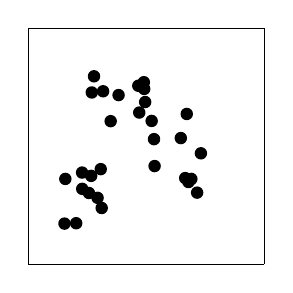
\begin{tikzpicture}[scale=1.5]
			\draw (0,0) -- (2,0);
			\draw (2,0) -- (2,2);
			\draw (2,2) -- (0,2);
			\draw (0,2) -- (0,0);
			
			\fill (0.456,0.778)circle (1.5pt);
			\fill (0.622,0.478)circle (1.5pt);
			\fill (0.457,0.64)circle (1.5pt);
			\fill (0.614,0.807)circle (1.5pt);
			\fill (0.314,0.724)circle (1.5pt);
			\fill (0.533,0.75)circle (1.5pt);
			\fill (0.514,0.605)circle (1.5pt);
			\fill (0.307,0.346)circle (1.5pt);
			\fill (0.406,0.349)circle (1.5pt);
			\fill (0.587,0.564)circle (1.5pt);
			
			\fill (1.065,1.061)circle (1.5pt);
			\fill (1.045,1.215)circle (1.5pt);
			\fill (1.292,1.07)circle (1.5pt);
			\fill (1.381,0.724)circle (1.5pt);
			\fill (1.43,0.608)circle (1.5pt);
			\fill (1.342,1.274)circle (1.5pt);
			\fill (1.329,0.731)circle (1.5pt);
			\fill (1.462,0.941)circle (1.5pt);
			\fill (1.357,0.698)circle (1.5pt);
			\fill (1.07,0.833)circle (1.5pt);
			
			\fill (0.765,1.434)circle (1.5pt);
			\fill (0.557,1.593)circle (1.5pt);
			\fill (0.698,1.213)circle (1.5pt);
			\fill (0.634,1.466)circle (1.5pt);
			\fill (0.979,1.543)circle (1.5pt);
			\fill (0.99,1.375)circle (1.5pt);
			\fill (0.538,1.456)circle (1.5pt);
			\fill (0.932,1.513)circle (1.5pt);
			\fill (0.982,1.486)circle (1.5pt);
			\fill (0.94,1.286)circle (1.5pt);
		\end{tikzpicture}
		\caption*{\footnotesize Original Set}
		\label{fig:badrep}
	\end{minipage}
	\begin{minipage}{0.4\linewidth}
		\centering
		\begin{tikzpicture}[scale=1.5]
		\draw (0,0) -- (2,0);
		\draw (2,0) -- (2,2);
		\draw (2,2) -- (0,2);
		\draw (0,2) -- (0,0);
		
		\fill (0.622,0.478)circle (1.5pt);
		\fill (1.462,0.941)circle (1.5pt);
		\fill (0.765,1.434)circle (1.5pt);
		\end{tikzpicture}		
		\caption*{\footnotesize Representative Set}
		\label{fig:goodrep}
	\end{minipage}
	\label{fig:rep}
\end{figure}
}

\frame{
	\frametitle{3. Geometric Disk Cover Problem}
	\framesubtitle{Approximation Algorithm - Chosing a distance}
	\begin{figure}[!h] 
  \begin{subfigure}[b]{0.24\linewidth}
		\centering
		\includegraphics[width=0.9\linewidth]{Pictures/sweden} 
		\caption{\small Original Set} 
		\label{fig:or_sweden} 
		\vspace{4ex}
  \end{subfigure}
  \begin{subfigure}[b]{0.24\linewidth}
    \centering
    \includegraphics[width=0.9\linewidth]{Pictures/10_sweden} 
	\caption{\small $d=10\%$} 
    \label{fig:10_sweden} 
    \vspace{4ex}
  \end{subfigure}%% 
  \begin{subfigure}[b]{0.24\linewidth}
    \centering
    \includegraphics[width=0.9\linewidth]{Pictures/15_sweden} 
    \caption{\small $d=15\%$} 
    \label{fig:15_sweden} 
    \vspace{4ex}
  \end{subfigure}
  \begin{subfigure}[b]{0.24\linewidth}
  	\centering
  	\includegraphics[width=0.9\linewidth]{Pictures/20_sweden} 
  	\caption{\small $d=20\%$} 
  	\label{fig:20_sweden} 
  	\vspace{4ex}
  \end{subfigure}
  \caption[Selected subsets from both graph building algorithms]{Selected subsets from both graph building algorithms.}
  \label{fig:sweden_dist} 
\end{figure}


}

\frame{
	\frametitle{3. Geometric Disk Cover Problem}
	\framesubtitle{Approximation Algorithm}
	\input{Figures/apx0}
	\begin{itemize}
		\item{Given $N$ points.}
	\end{itemize}
}

\frame{
	\frametitle{3. Geometric Disk Cover Problem}
	\framesubtitle{Approximation Algorithm}
	\begin{figure}[H]
	\begin{center}
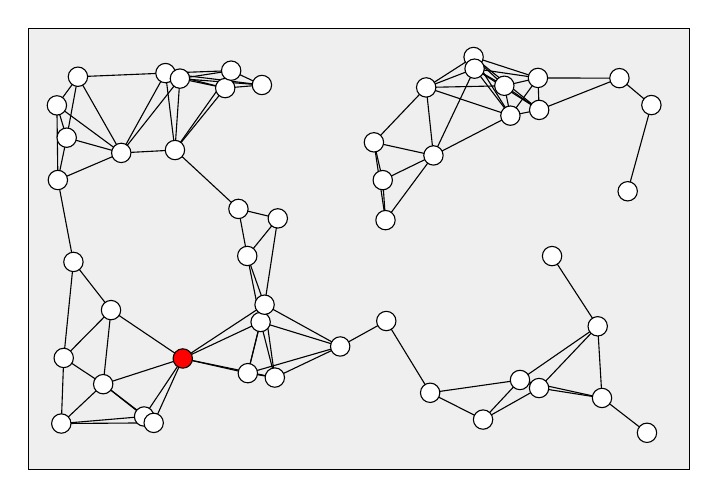
\begin{tikzpicture}[scale=1.4]
\fill[lightgray!25,draw=black] (0,0) rectangle (6,4);
\clip (0,0) rectangle (6,4);-
\draw [](0.26,3.3) -- (0.269,2.623);
\draw [](0.26,3.3) -- (0.349,3.007);
\draw [](0.26,3.3) -- (0.451,3.56);
\draw [](0.26,3.3) -- (0.844,2.869);
\draw [](0.269,2.623) -- (0.349,3.007);
\draw [](0.269,2.623) -- (0.41,1.88);
\draw [](0.269,2.623) -- (0.844,2.869);
\draw [](0.3,0.414) -- (0.322,1.009);
\draw [](0.3,0.414) -- (0.68,0.771);
\draw [](0.3,0.414) -- (1.051,0.478);
\draw [](0.3,0.414) -- (1.138,0.42);
\draw [](0.322,1.009) -- (0.41,1.88);
\draw [](0.322,1.009) -- (0.68,0.771);
\draw [](0.322,1.009) -- (0.751,1.443);
\draw [](0.349,3.007) -- (0.451,3.56);
\draw [](0.349,3.007) -- (0.844,2.869);
\draw [](0.41,1.88) -- (0.751,1.443);
\draw [](0.451,3.56) -- (0.844,2.869);
\draw [](0.451,3.56) -- (1.245,3.593);
\draw [](0.68,0.771) -- (0.751,1.443);
\draw [](0.68,0.771) -- (1.051,0.478);
\draw [](0.68,0.771) -- (1.138,0.42);
\draw [](0.68,0.771) -- (1.402,1.004);
\draw [](0.751,1.443) -- (1.402,1.004);
\draw [](0.844,2.869) -- (1.245,3.593);
\draw [](0.844,2.869) -- (1.331,2.895);
\draw [](0.844,2.869) -- (1.376,3.543);
\draw [](1.051,0.478) -- (1.138,0.42);
\draw [](1.051,0.478) -- (1.402,1.004);
\draw [](1.138,0.42) -- (1.402,1.004);
\draw [](1.245,3.593) -- (1.331,2.895);
\draw [](1.245,3.593) -- (1.376,3.543);
\draw [](1.245,3.593) -- (1.787,3.457);
\draw [](1.245,3.593) -- (1.841,3.615);
\draw [](1.245,3.593) -- (2.12,3.485);
\draw [](1.331,2.895) -- (1.376,3.543);
\draw [](1.331,2.895) -- (1.787,3.457);
\draw [](1.331,2.895) -- (1.841,3.615);
\draw [](1.331,2.895) -- (1.907,2.361);
\draw [](1.376,3.543) -- (1.787,3.457);
\draw [](1.376,3.543) -- (1.841,3.615);
\draw [](1.376,3.543) -- (2.12,3.485);
\draw [](1.402,1.004) -- (1.992,0.871);
\draw [](1.402,1.004) -- (2.108,1.335);
\draw [](1.402,1.004) -- (2.144,1.492);
\draw [](1.402,1.004) -- (2.237,0.831);
\draw [](1.787,3.457) -- (1.841,3.615);
\draw [](1.787,3.457) -- (2.12,3.485);
\draw [](1.841,3.615) -- (2.12,3.485);
\draw [](1.907,2.361) -- (1.987,1.934);
\draw [](1.907,2.361) -- (2.264,2.275);
\draw [](1.987,1.934) -- (2.108,1.335);
\draw [](1.987,1.934) -- (2.144,1.492);
\draw [](1.987,1.934) -- (2.264,2.275);
\draw [](1.992,0.871) -- (2.108,1.335);
\draw [](1.992,0.871) -- (2.144,1.492);
\draw [](1.992,0.871) -- (2.237,0.831);
\draw [](1.992,0.871) -- (2.83,1.113);
\draw [](2.108,1.335) -- (2.144,1.492);
\draw [](2.108,1.335) -- (2.237,0.831);
\draw [](2.108,1.335) -- (2.83,1.113);
\draw [](2.144,1.492) -- (2.237,0.831);
\draw [](2.144,1.492) -- (2.264,2.275);
\draw [](2.144,1.492) -- (2.83,1.113);
\draw [](2.237,0.831) -- (2.83,1.113);
\draw [](2.83,1.113) -- (3.248,1.344);
\draw [](3.136,2.965) -- (3.216,2.622);
\draw [](3.136,2.965) -- (3.241,2.259);
\draw [](3.136,2.965) -- (3.61,3.463);
\draw [](3.136,2.965) -- (3.676,2.846);
\draw [](3.216,2.622) -- (3.241,2.259);
\draw [](3.216,2.622) -- (3.676,2.846);
\draw [](3.241,2.259) -- (3.676,2.846);
\draw [](3.248,1.344) -- (3.646,0.693);
\draw [](3.61,3.463) -- (3.676,2.846);
\draw [](3.61,3.463) -- (4.04,3.739);
\draw [](3.61,3.463) -- (4.049,3.633);
\draw [](3.61,3.463) -- (4.319,3.478);
\draw [](3.61,3.463) -- (4.374,3.207);
\draw [](3.646,0.693) -- (4.126,0.45);
\draw [](3.646,0.693) -- (4.461,0.809);
\draw [](3.676,2.846) -- (4.049,3.633);
\draw [](3.676,2.846) -- (4.374,3.207);
\draw [](4.04,3.739) -- (4.049,3.633);
\draw [](4.04,3.739) -- (4.319,3.478);
\draw [](4.04,3.739) -- (4.374,3.207);
\draw [](4.04,3.739) -- (4.624,3.549);
\draw [](4.04,3.739) -- (4.635,3.259);
\draw [](4.049,3.633) -- (4.319,3.478);
\draw [](4.049,3.633) -- (4.374,3.207);
\draw [](4.049,3.633) -- (4.624,3.549);
\draw [](4.049,3.633) -- (4.635,3.259);
\draw [](4.126,0.45) -- (4.461,0.809);
\draw [](4.126,0.45) -- (4.634,0.736);
\draw [](4.319,3.478) -- (4.374,3.207);
\draw [](4.319,3.478) -- (4.624,3.549);
\draw [](4.319,3.478) -- (4.635,3.259);
\draw [](4.374,3.207) -- (4.624,3.549);
\draw [](4.374,3.207) -- (4.635,3.259);
\draw [](4.461,0.809) -- (4.634,0.736);
\draw [](4.461,0.809) -- (5.166,1.296);
\draw [](4.461,0.809) -- (5.205,0.646);
\draw [](4.624,3.549) -- (4.635,3.259);
\draw [](4.624,3.549) -- (5.363,3.547);
\draw [](4.634,0.736) -- (5.166,1.296);
\draw [](4.634,0.736) -- (5.205,0.646);
\draw [](4.635,3.259) -- (5.363,3.547);
\draw [](4.752,1.933) -- (5.166,1.296);
\draw [](5.166,1.296) -- (5.205,0.646);
\draw [](5.205,0.646) -- (5.613,0.33);
\draw [](5.363,3.547) -- (5.653,3.303);
\draw [](5.438,2.521) -- (5.653,3.303);
\fill [white,draw=black] (0.26,3.3) circle (2.5pt);
\fill [white,draw=black] (0.269,2.623) circle (2.5pt);
\fill [white,draw=black] (0.3,0.414) circle (2.5pt);
\fill [white,draw=black] (0.322,1.009) circle (2.5pt);
\fill [white,draw=black] (0.349,3.007) circle (2.5pt);
\fill [white,draw=black] (0.41,1.88) circle (2.5pt);
\fill [white,draw=black] (0.451,3.56) circle (2.5pt);
\fill [white,draw=black] (0.68,0.771) circle (2.5pt);
\fill [white,draw=black] (0.751,1.443) circle (2.5pt);
\fill [white,draw=black] (0.844,2.869) circle (2.5pt);
\fill [white,draw=black] (1.051,0.478) circle (2.5pt);
\fill [white,draw=black] (1.138,0.42) circle (2.5pt);
\fill [white,draw=black] (1.245,3.593) circle (2.5pt);
\fill [white,draw=black] (1.331,2.895) circle (2.5pt);
\fill [white,draw=black] (1.376,3.543) circle (2.5pt);
\node [red] at (1.402,1.004) {\tiny $8$};
\fill [red,draw=black] (1.402,1.004) circle (2.5pt);
\fill [white,draw=black] (1.787,3.457) circle (2.5pt);
\fill [white,draw=black] (1.841,3.615) circle (2.5pt);
\fill [white,draw=black] (1.907,2.361) circle (2.5pt);
\fill [white,draw=black] (1.987,1.934) circle (2.5pt);
\fill [white,draw=black] (1.992,0.871) circle (2.5pt);
\fill [white,draw=black] (2.108,1.335) circle (2.5pt);
\fill [white,draw=black] (2.12,3.485) circle (2.5pt);
\fill [white,draw=black] (2.144,1.492) circle (2.5pt);
\fill [white,draw=black] (2.237,0.831) circle (2.5pt);
\fill [white,draw=black] (2.264,2.275) circle (2.5pt);
\fill [white,draw=black] (2.83,1.113) circle (2.5pt);
\fill [white,draw=black] (3.136,2.965) circle (2.5pt);
\fill [white,draw=black] (3.216,2.622) circle (2.5pt);
\fill [white,draw=black] (3.241,2.259) circle (2.5pt);
\fill [white,draw=black] (3.248,1.344) circle (2.5pt);
\fill [white,draw=black] (3.61,3.463) circle (2.5pt);
\fill [white,draw=black] (3.646,0.693) circle (2.5pt);
\fill [white,draw=black] (3.676,2.846) circle (2.5pt);
\fill [white,draw=black] (4.04,3.739) circle (2.5pt);
\fill [white,draw=black] (4.049,3.633) circle (2.5pt);
\fill [white,draw=black] (4.126,0.45) circle (2.5pt);
\fill [white,draw=black] (4.319,3.478) circle (2.5pt);
\fill [white,draw=black] (4.374,3.207) circle (2.5pt);
\fill [white,draw=black] (4.461,0.809) circle (2.5pt);
\fill [white,draw=black] (4.624,3.549) circle (2.5pt);
\fill [white,draw=black] (4.634,0.736) circle (2.5pt);
\fill [white,draw=black] (4.635,3.259) circle (2.5pt);
\fill [white,draw=black] (4.752,1.933) circle (2.5pt);
\fill [white,draw=black] (5.166,1.296) circle (2.5pt);
\fill [white,draw=black] (5.205,0.646) circle (2.5pt);
\fill [white,draw=black] (5.363,3.547) circle (2.5pt);
\fill [white,draw=black] (5.438,2.521) circle (2.5pt);
\fill [white,draw=black] (5.613,0.33) circle (2.5pt);
\fill [white,draw=black] (5.653,3.303) circle (2.5pt);
\end{tikzpicture}

\end{center}
\caption{Illustration of the graph. The number in red represents the point with the largest number of neighbours.}
\label{fig:aa1}
\end{figure}

	\begin{itemize}
		\item Connect all pairs whose distance is less than $d$ 
	\end{itemize}
}

\frame{
	\frametitle{3. Geometric Disk Cover Problem}
	\framesubtitle{Approximation Algorithm}
	\begin{figure}[!h]
\begin{center}
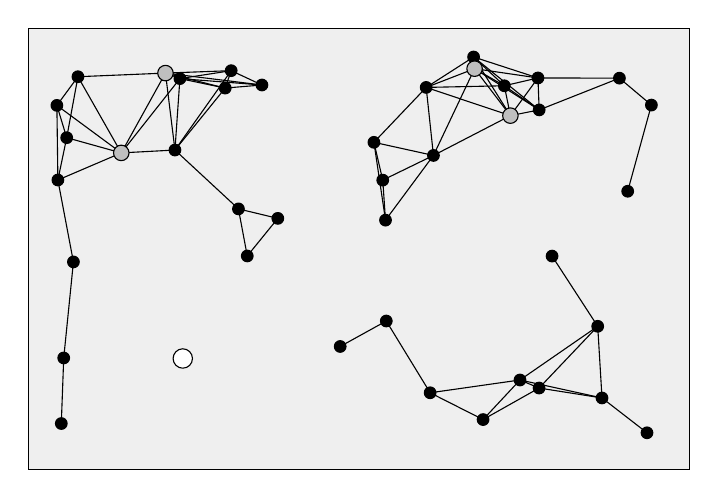
\begin{tikzpicture}[scale=1.4]
\fill[lightgray!25,draw=black] (0,0) rectangle (6,4);
\clip (0,0) rectangle (6,4);
\draw [](0.26,3.3) -- (0.269,2.623);
\draw [](0.26,3.3) -- (0.349,3.007);
\draw [](0.26,3.3) -- (0.451,3.56);
\draw [](0.26,3.3) -- (0.844,2.869);
\draw [](0.269,2.623) -- (0.349,3.007);
\draw [](0.269,2.623) -- (0.41,1.88);
\draw [](0.269,2.623) -- (0.844,2.869);
\draw [](0.3,0.414) -- (0.322,1.009);
\draw [](0.322,1.009) -- (0.41,1.88);
\draw [](0.349,3.007) -- (0.451,3.56);
\draw [](0.349,3.007) -- (0.844,2.869);
\draw [](0.451,3.56) -- (0.844,2.869);
\draw [](0.451,3.56) -- (1.245,3.593);
\draw [](0.844,2.869) -- (1.245,3.593);
\draw [](0.844,2.869) -- (1.331,2.895);
\draw [](0.844,2.869) -- (1.376,3.543);
\draw [](1.245,3.593) -- (1.331,2.895);
\draw [](1.245,3.593) -- (1.376,3.543);
\draw [](1.245,3.593) -- (1.787,3.457);
\draw [](1.245,3.593) -- (1.841,3.615);
\draw [](1.245,3.593) -- (2.12,3.485);
\draw [](1.331,2.895) -- (1.376,3.543);
\draw [](1.331,2.895) -- (1.787,3.457);
\draw [](1.331,2.895) -- (1.841,3.615);
\draw [](1.331,2.895) -- (1.907,2.361);
\draw [](1.376,3.543) -- (1.787,3.457);
\draw [](1.376,3.543) -- (1.841,3.615);
\draw [](1.376,3.543) -- (2.12,3.485);
\draw [](1.787,3.457) -- (1.841,3.615);
\draw [](1.787,3.457) -- (2.12,3.485);
\draw [](1.841,3.615) -- (2.12,3.485);
\draw [](1.907,2.361) -- (1.987,1.934);
\draw [](1.907,2.361) -- (2.264,2.275);
\draw [](1.987,1.934) -- (2.264,2.275);
\draw [](2.83,1.113) -- (3.248,1.344);
\draw [](3.136,2.965) -- (3.216,2.622);
\draw [](3.136,2.965) -- (3.241,2.259);
\draw [](3.136,2.965) -- (3.61,3.463);
\draw [](3.136,2.965) -- (3.676,2.846);
\draw [](3.216,2.622) -- (3.241,2.259);
\draw [](3.216,2.622) -- (3.676,2.846);
\draw [](3.241,2.259) -- (3.676,2.846);
\draw [](3.248,1.344) -- (3.646,0.693);
\draw [](3.61,3.463) -- (3.676,2.846);
\draw [](3.61,3.463) -- (4.04,3.739);
\draw [](3.61,3.463) -- (4.049,3.633);
\draw [](3.61,3.463) -- (4.319,3.478);
\draw [](3.61,3.463) -- (4.374,3.207);
\draw [](3.646,0.693) -- (4.126,0.45);
\draw [](3.646,0.693) -- (4.461,0.809);
\draw [](3.676,2.846) -- (4.049,3.633);
\draw [](3.676,2.846) -- (4.374,3.207);
\draw [](4.04,3.739) -- (4.049,3.633);
\draw [](4.04,3.739) -- (4.319,3.478);
\draw [](4.04,3.739) -- (4.374,3.207);
\draw [](4.04,3.739) -- (4.624,3.549);
\draw [](4.04,3.739) -- (4.635,3.259);
\draw [](4.049,3.633) -- (4.319,3.478);
\draw [](4.049,3.633) -- (4.374,3.207);
\draw [](4.049,3.633) -- (4.624,3.549);
\draw [](4.049,3.633) -- (4.635,3.259);
\draw [](4.126,0.45) -- (4.461,0.809);
\draw [](4.126,0.45) -- (4.634,0.736);
\draw [](4.319,3.478) -- (4.374,3.207);
\draw [](4.319,3.478) -- (4.624,3.549);
\draw [](4.319,3.478) -- (4.635,3.259);
\draw [](4.374,3.207) -- (4.624,3.549);
\draw [](4.374,3.207) -- (4.635,3.259);
\draw [](4.461,0.809) -- (4.634,0.736);
\draw [](4.461,0.809) -- (5.166,1.296);
\draw [](4.461,0.809) -- (5.205,0.646);
\draw [](4.624,3.549) -- (4.635,3.259);
\draw [](4.624,3.549) -- (5.363,3.547);
\draw [](4.634,0.736) -- (5.166,1.296);
\draw [](4.634,0.736) -- (5.205,0.646);
\draw [](4.635,3.259) -- (5.363,3.547);
\draw [](4.752,1.933) -- (5.166,1.296);
\draw [](5.166,1.296) -- (5.205,0.646);
\draw [](5.205,0.646) -- (5.613,0.33);
\draw [](5.363,3.547) -- (5.653,3.303);
\draw [](5.438,2.521) -- (5.653,3.303);
\fill [black,draw=black] (0.26,3.3) circle (1.5pt);
\fill [black,draw=black] (0.269,2.623) circle (1.5pt);
\fill [black,draw=black] (0.3,0.414) circle (1.5pt);
\fill [black,draw=black] (0.322,1.009) circle (1.5pt);
\fill [black,draw=black] (0.349,3.007) circle (1.5pt);
\fill [black,draw=black] (0.41,1.88) circle (1.5pt);
\fill [black,draw=black] (0.451,3.56) circle (1.5pt);
\fill [black,draw=black] (0.844,2.869) circle (1.5pt);
\fill [black,draw=black] (1.245,3.593) circle (1.5pt);
\fill [black,draw=black] (1.331,2.895) circle (1.5pt);
\fill [black,draw=black] (1.376,3.543) circle (1.5pt);
\fill [black,draw=black] (1.787,3.457) circle (1.5pt);
\fill [black,draw=black] (1.841,3.615) circle (1.5pt);
\fill [black,draw=black] (1.907,2.361) circle (1.5pt);
\fill [black,draw=black] (1.987,1.934) circle (1.5pt);
\fill [black,draw=black] (2.12,3.485) circle (1.5pt);
\fill [black,draw=black] (2.264,2.275) circle (1.5pt);
\fill [black,draw=black] (2.83,1.113) circle (1.5pt);
\fill [black,draw=black] (3.136,2.965) circle (1.5pt);
\fill [black,draw=black] (3.216,2.622) circle (1.5pt);
\fill [black,draw=black] (3.241,2.259) circle (1.5pt);
\fill [black,draw=black] (3.248,1.344) circle (1.5pt);
\fill [black,draw=black] (3.61,3.463) circle (1.5pt);
\fill [black,draw=black] (3.646,0.693) circle (1.5pt);
\fill [black,draw=black] (3.676,2.846) circle (1.5pt);
\fill [black,draw=black] (4.04,3.739) circle (1.5pt);
\fill [black,draw=black] (4.049,3.633) circle (1.5pt);
\fill [black,draw=black] (4.126,0.45) circle (1.5pt);
\fill [black,draw=black] (4.319,3.478) circle (1.5pt);
\fill [black,draw=black] (4.374,3.207) circle (1.5pt);
\fill [black,draw=black] (4.461,0.809) circle (1.5pt);
\fill [black,draw=black] (4.624,3.549) circle (1.5pt);
\fill [black,draw=black] (4.634,0.736) circle (1.5pt);
\fill [black,draw=black] (4.635,3.259) circle (1.5pt);
\fill [black,draw=black] (4.752,1.933) circle (1.5pt);
\fill [black,draw=black] (5.166,1.296) circle (1.5pt);
\fill [black,draw=black] (5.205,0.646) circle (1.5pt);
\fill [black,draw=black] (5.363,3.547) circle (1.5pt);
\fill [black,draw=black] (5.438,2.521) circle (1.5pt);
\fill [black,draw=black] (5.613,0.33) circle (1.5pt);
\fill [black,draw=black] (5.653,3.303) circle (1.5pt);

\fill [lightgray,draw=black] (0.844,2.869) circle (2pt);
%\node [red] at (0.844,2.869) {\tiny $7$};
\fill [lightgray,draw=black] (1.245,3.593) circle (2pt);
%\node [red] at (1.245,3.593) {\tiny $7$};
\fill [lightgray,draw=black] (4.049,3.633) circle (2pt);
%\node [red] at (4.049,3.633) {\tiny $7$};
\fill [lightgray,draw=black] (4.374,3.207) circle (2pt);
%\node [red] at (4.374,3.207) {\tiny $7$};
\fill [white,draw=black] (1.402,1.004) circle (2.5pt);
\end{tikzpicture}

\end{center}
\caption[Illustration of the state of the proximity graph after the first iteration.]{Illustration of the state of the proximity graph after the first iteration. Any of the gray points is to be removed in the next iteration, as they have the largest amount of neighbours.}
\label{fig:aa2}
\end{figure}

	\begin{itemize}
		\item{Select point with most connections and remove its neighbours.}
	\end{itemize}
}

\frame{
	\frametitle{3. Geometric Disk Cover Problem}
	\framesubtitle{Approximation Algorithm}
	\begin{figure}[H]
\begin{center}
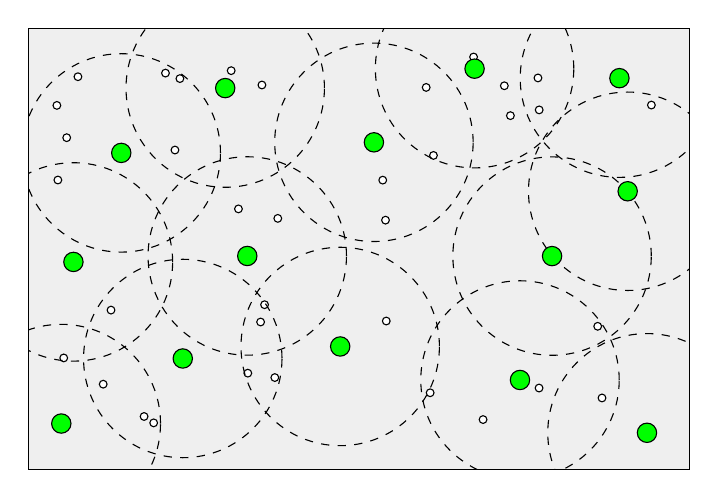
\begin{tikzpicture}[scale=1.4]
\fill[lightgray!25,draw=black] (0,0) rectangle (6,4);
\clip (0,0) rectangle (6,4);


\fill [white,draw=black] (0.26,3.3) circle (1pt);
\fill [white,draw=black] (0.269,2.623) circle (1pt);
\fill [white,draw=black] (0.3,0.414) circle (1pt);
\fill [white,draw=black] (0.322,1.009) circle (1pt);
\fill [white,draw=black] (0.349,3.007) circle (1pt);
\fill [white,draw=black] (0.41,1.88) circle (1pt);
\fill [white,draw=black] (0.451,3.56) circle (1pt);
\fill [white,draw=black] (0.68,0.771) circle (1pt);
\fill [white,draw=black] (0.751,1.443) circle (1pt);
\fill [white,draw=black] (0.844,2.869) circle (1pt);
\fill [white,draw=black] (1.051,0.478) circle (1pt);
\fill [white,draw=black] (1.138,0.42) circle (1pt);
\fill [white,draw=black] (1.245,3.593) circle (1pt);
\fill [white,draw=black] (1.331,2.895) circle (1pt);
\fill [white,draw=black] (1.376,3.543) circle (1pt);
\fill [white,draw=black] (1.402,1.004) circle (1pt);
\fill [white,draw=black] (1.787,3.457) circle (1pt);
\fill [white,draw=black] (1.841,3.615) circle (1pt);
\fill [white,draw=black] (1.907,2.361) circle (1pt);
\fill [white,draw=black] (1.987,1.934) circle (1pt);
\fill [white,draw=black] (1.992,0.871) circle (1pt);
\fill [white,draw=black] (2.108,1.335) circle (1pt);
\fill [white,draw=black] (2.12,3.485) circle (1pt);
\fill [white,draw=black] (2.144,1.492) circle (1pt);
\fill [white,draw=black] (2.237,0.831) circle (1pt);
\fill [white,draw=black] (2.264,2.275) circle (1pt);
\fill [white,draw=black] (2.83,1.113) circle (1pt);
\fill [white,draw=black] (3.136,2.965) circle (1pt);
\fill [white,draw=black] (3.216,2.622) circle (1pt);
\fill [white,draw=black] (3.241,2.259) circle (1pt);
\fill [white,draw=black] (3.248,1.344) circle (1pt);
\fill [white,draw=black] (3.61,3.463) circle (1pt);
\fill [white,draw=black] (3.646,0.693) circle (1pt);
\fill [white,draw=black] (3.676,2.846) circle (1pt);
\fill [white,draw=black] (4.04,3.739) circle (1pt);
\fill [white,draw=black] (4.049,3.633) circle (1pt);
\fill [white,draw=black] (4.126,0.45) circle (1pt);
\fill [white,draw=black] (4.319,3.478) circle (1pt);
\fill [white,draw=black] (4.374,3.207) circle (1pt);
\fill [white,draw=black] (4.461,0.809) circle (1pt);
\fill [white,draw=black] (4.624,3.549) circle (1pt);
\fill [white,draw=black] (4.634,0.736) circle (1pt);
\fill [white,draw=black] (4.635,3.259) circle (1pt);
\fill [white,draw=black] (4.752,1.933) circle (1pt);
\fill [white,draw=black] (5.166,1.296) circle (1pt);
\fill [white,draw=black] (5.205,0.646) circle (1pt);
\fill [white,draw=black] (5.363,3.547) circle (1pt);
\fill [white,draw=black] (5.438,2.521) circle (1pt);
\fill [white,draw=black] (5.613,0.33) circle (1pt);
\fill [white,draw=black] (5.653,3.303) circle (1pt);

\draw [dashed] (1.402,1.004) circle (0.9);
\draw [dashed] (0.844,2.869) circle (0.9);
\draw [dashed] (4.049,3.633) circle (0.9);
\draw [dashed] (1.787,3.457) circle (0.9);
\draw [dashed] (2.83,1.113) circle (0.9);
\draw [dashed] (4.461,0.809) circle (0.9);
\draw [dashed] (0.3,0.414) circle (0.9);
\draw [dashed] (1.987,1.934) circle (0.9);
\draw [dashed] (3.136,2.965) circle (0.9);
\draw [dashed] (0.41,1.88) circle (0.9);
\draw [dashed] (5.363,3.547) circle (0.9);
\draw [dashed] (4.752,1.933) circle (0.9);
\draw [dashed] (5.438,2.521) circle (0.9);
\draw [dashed] (5.613,0.33) circle (0.9);

\fill [green,draw=black] (1.402,1.004) circle (2.5pt);
%\node [black] at (1.402,1.004) {\tiny $1$};
\fill [green,draw=black] (0.844,2.869) circle (2.5pt);
%\node [black] at (0.844,2.869) {\tiny $2$};
\fill [green,draw=black] (4.049,3.633) circle (2.5pt);
%\node [black] at (4.049,3.633) {\tiny $3$};
\fill [green,draw=black] (1.787,3.457) circle (2.5pt);
%\node [black] at (1.787,3.457) {\tiny $4$};
\fill [green,draw=black] (2.83,1.113) circle (2.5pt);
%\node [black] at (2.83,1.113) {\tiny $5$};
\fill [green,draw=black] (4.461,0.809) circle (2.5pt);
%\node [black] at (4.461,0.809) {\tiny $6$};
\fill [green,draw=black] (0.3,0.414) circle (2.5pt);
%\node [black] at (0.3,0.414) {\tiny $7$};
\fill [green,draw=black] (1.987,1.934) circle (2.5pt);
%\node [black] at (1.987,1.934) {\tiny $8$};
\fill [green,draw=black] (3.136,2.965) circle (2.5pt);
%\node [black] at (3.136,2.965) {\tiny $9$};
\fill [green,draw=black] (0.41,1.88) circle (2.5pt);
%\node [black] at (0.41,1.88) {\tiny $10$};
\fill [green,draw=black] (5.363,3.547) circle (2.5pt);
%\node [black] at (5.363,3.547) {\tiny $11$};
\fill [green,draw=black] (4.752,1.933) circle (2.5pt);
%\node [black] at (4.752,1.933) {\tiny $12$};
\fill [green,draw=black] (5.438,2.521) circle (2.5pt);
%\node [black] at (5.438,2.521) {\tiny $13$};
\fill [green,draw=black] (5.613,0.33) circle (2.5pt);
%\node [black] at (5.613,0.33) {\tiny $14$};

\end{tikzpicture}

\end{center}
\caption[Illustration of the state of the final chosen set]{Illustration of the state of the final chosen set. The green points are the final representative set.}
\label{fig:aa3}


\end{figure}

	\begin{itemize}
		\item{Repeat until all points are either removed or selected.}
	\end{itemize}
}

%\frame{
%	\frametitle{Geometric Disk Cover}
%	\framesubtitle{Buiding the Proximity Graph}
%	\input{Figures/kd1}
%}
%
%\frame{
%	\frametitle{Geometric Disk Cover}
%	\framesubtitle{Buiding the Proximity Graph}
%	\begin{figure}[H]
	\begin{center}
		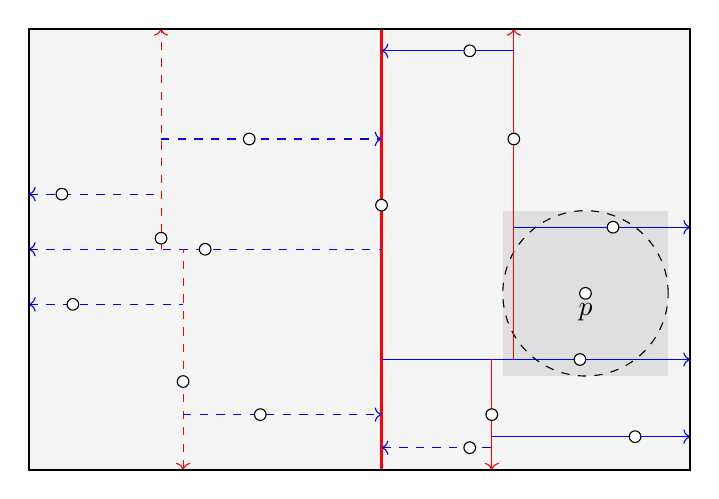
\begin{tikzpicture}[scale=1.4]
		\fill[lightgray!15] (0,0) rectangle (6,4);
		\fill[lightgray!50] (4.3,0.85) rectangle (5.8,2.35);
		\draw[dashed](5.05,1.6) circle(0.75);
		\fill[white,draw=black] (5.05,1.6) circle(1.5pt);
		\node[below] at (5.05,1.6) {$\tiny p$};
		
		\draw [red,thick](3.2,0) -- (3.2,4);
		\fill[white,draw=black] (3.2,2.4) circle (1.5pt);
		\draw [blue,->](3.2,1) -- (6,1);
		\fill[white,draw=black] (5,1) circle (1.5pt);
		\draw [red,<-](4.2,0) -- (4.2,1);
		\fill[white,draw=black] (4.2,0.5) circle (1.5pt);
		\draw [blue,<-,dashed](3.2,0.2) -- (4.2,0.2);
		\fill[white,draw=black] (4,0.2) circle (1.5pt);
		\draw [blue,->](4.2,0.3) -- (6,0.3);
		\fill[white,draw=black] (5.5,0.3) circle (1.5pt);
		\draw [red,->](4.4,1) -- (4.4,4);
		\fill[white,draw=black] (4.4,3) circle (1.5pt);
		\draw [blue,<-](3.2,3.8) -- (4.4,3.8);
		\fill[white,draw=black] (4,3.8) circle (1.5pt);
		\draw [blue,->](4.4,2.2) -- (6,2.2);
		\fill[white,draw=black] (5.3,2.2) circle (1.5pt);
		\draw [blue,<-,dashed](0,2) -- (3.2,2);
		\fill[white,draw=black] (1.6,2) circle (1.5pt);
		\draw [red,->,dashed](1.2,2) -- (1.2,4);
		\fill[white,draw=black] (1.2,2.1) circle (1.5pt);
		\draw [blue,->,dashed](1.2,3) -- (3.2,3);
		\fill[white,draw=black] (2,3) circle (1.5pt);
		\draw [blue,<-,dashed](0,2.5) -- (1.2,2.5);
		\fill[white,draw=black] (0.3,2.5) circle (1.5pt);
		\draw [red,<-,dashed](1.4,0) -- (1.4,2);
		\fill[white,draw=black] (1.4,0.8) circle (1.5pt);
		\draw [blue,->,dashed](1.4,0.5) -- (3.2,0.5);
		\fill[white,draw=black] (2.1,0.5) circle (1.5pt);
		\draw [blue,<-,dashed](0,1.5) -- (1.4,1.5);
		\fill[white,draw=black] (0.4,1.5) circle (1.5pt);
		\draw[thick] (0,0) rectangle (6,4);
		\end{tikzpicture}
	\end{center}
	\caption[Example of a range search query on a \kdTree] {The dashed lines are never queried, since the rectangle does not intercept their parent. This query searches for all points within a fixed distance of $p$.}
	\label{fig:kdrs}
\end{figure}
%}
%
%\frame{
%	\frametitle{Geometric Disk Cover}
%	\framesubtitle{Buiding the Proximity Graph}
%	\begin{figure}[H]
\begin{center}
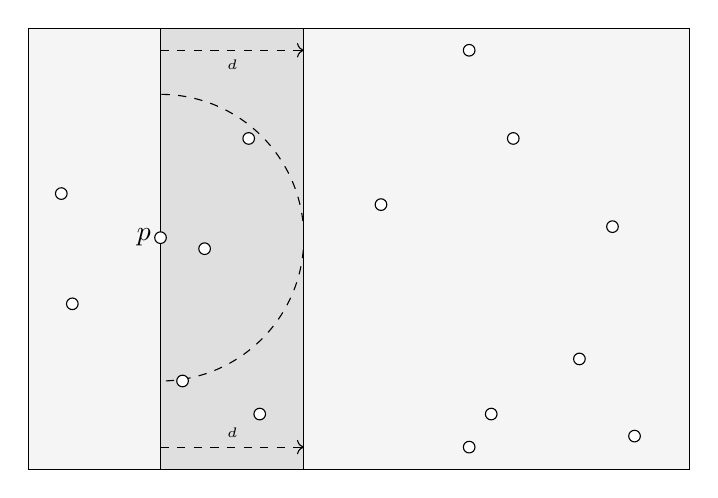
\begin{tikzpicture}[scale=1.4]
	\fill[lightgray!15,draw=black] (0,0) rectangle (6,4);
	\fill[lightgray!50,draw=black] (1.2,0) rectangle (2.5,4);
	\begin{scope}
	\clip (1.2,0) rectangle (2.5,4);
	\draw[dashed](1.2,2.1) circle (1.3);
	\end{scope}
	
	\draw [dashed,->](1.2,0.2) -- node[above]{\tiny$d$}(2.5,0.2);

	\draw [dashed,->](1.2,3.8) -- node[below]{\tiny$d$}(2.5,3.8);

	\node[left] at (1.2,2.1) {$\tiny p$};

	\fill[white,draw=black] (3.2,2.4) circle (1.5pt);
	\fill[white,draw=black] (5,1) circle (1.5pt);		
	\fill[white,draw=black] (4.2,0.5) circle (1.5pt);
	\fill[white,draw=black] (4,0.2) circle (1.5pt);
	\fill[white,draw=black] (5.5,0.3) circle (1.5pt);
	\fill[white,draw=black] (4.4,3) circle (1.5pt);
	\fill[white,draw=black] (4,3.8) circle (1.5pt);
	\fill[white,draw=black] (5.3,2.2) circle (1.5pt);
	\fill[white,draw=black] (1.6,2) circle (1.5pt);
	\fill[white,draw=black] (1.2,2.1) circle (1.5pt);
	\fill[white,draw=black] (2,3) circle (1.5pt);
	\fill[white,draw=black] (0.3,2.5) circle (1.5pt);
	\fill[white,draw=black] (1.4,0.8) circle (1.5pt);
	\fill[white,draw=black] (2.1,0.5) circle (1.5pt);
	\fill[white,draw=black] (0.4,1.5) circle (1.5pt);

\end{tikzpicture}
\end{center}
\caption[Illustration of the Line Sweep method.]{Illustration of the Line Sweep method. This query searches for the points within a given distance of $p$ that are to the right of $p$}
\label{fig:ls1}
\end{figure}
%}

\frame{
	\frametitle{3. Geometric Disk Cover Problem}
	\framesubtitle{$k$-d Trees vs. Line Sweep}
	\begin{figure}[!h] 
	\centering 
    \includegraphics[width=\linewidth]{Pictures/ls_kd_t}
    \label{fig:ls_kd_t} 
\end{figure}


	\begin{itemize}
		\item{Line Sweep algorithm is faster.}
	\end{itemize}
}



\frame{
	\frametitle{3. Geometric Disk Cover Problem}
	\framesubtitle{$k$-d Trees vs. Line Sweep}
	\begin{figure}[!h] 
	\centering 
	\vspace{-10pt}
    \includegraphics[width=\linewidth]{Pictures/ls_kd_s}
    \label{fig:ls_kd_s} 
\end{figure}


	\begin{itemize}
		\item{Both algorithms use the same space (up to 4Gb)}
	\end{itemize}
}

\frame{
	\frametitle{3. Geometric Disk Cover Problem}
	\framesubtitle{$k$-d Trees vs. Line Sweep}
	\begin{figure}[!h] 
	\centering
	\includegraphics[width=0.8\linewidth]{Pictures/ls_kd_k} 
	\caption[Number $k$ of points selected for Line Sweep and $k$-d Tree range search.]{Number $k$ of points selected for both proximity graph algorithms on uniform and clustered inputs for different values of $d$.}
	\label{fig:ls_kd_k} 
\end{figure}
	\begin{itemize}
		\item{Both algorithms give the same results}
	\end{itemize}
}

\frame{
	\frametitle{3. Geometric Disk Cover Problem}
	\framesubtitle{Heuristic Speed-ups: Random Sampling}
	\begin{itemize}
		\item Randomly discard a fraction of the input points.
		\item Uniform sets should keep a similar distribution.
		\item Less points to deal means faster times.
	\end{itemize}
	\pause
	\begin{figure}[!h] 
  \centering
  \begin{subfigure}[b]{0.45\linewidth}
    \centering
    \includegraphics[width=0.9\linewidth]{Pictures/rs_greece} 
    %\caption{$N=10$} 
    \label{fig:ls_greece} 
  \end{subfigure}%% 
  \begin{subfigure}[b]{0.45\linewidth}
    \centering
    \includegraphics[width=0.9\linewidth]{Pictures/ls_greece} 
    %\caption{$N=20$} 
    \label{fig:rs_greece} 
  \end{subfigure}
  \label{fig:ls_rs_greece} 
\end{figure}


}

\frame{
	\frametitle{3. Geometric Disk Cover Problem}
	\framesubtitle{Heuristic Speed-ups: Two-Phase Filtering}
	\begin{itemize}
		\item Solve the problem with a smaller distance first.
		\item Use the output as a new input for the given distance.
		\item Sparser graphs mean faster CPU times.
	\end{itemize}
	\pause
	\begin{figure}[!h]
\begin{center}
	
	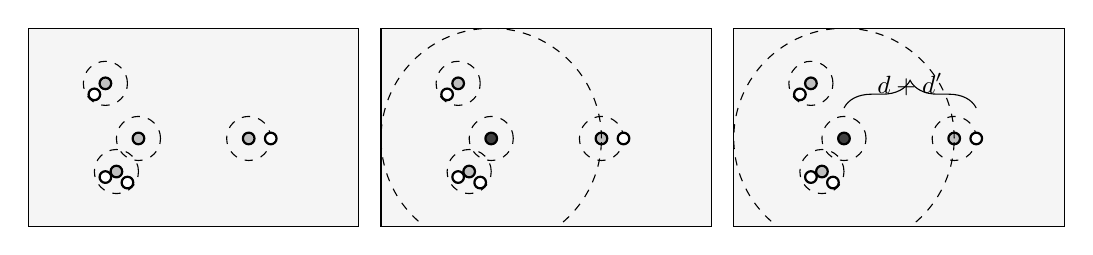
\begin{tikzpicture}[scale=1.4]
%	\begin{scope}[]
%	\fill[lightgray!15,draw=black] (-1,-0.8) rectangle (2,1);
%	\fill[white,draw=black,thick] (0,0) circle (1.5pt);
%	\fill[white,draw=black,thick] (1,0) circle (1.5pt);
%	\fill[white,draw=black,thick] (1.2,0) circle (1.5pt);
%	
%	\fill[white,draw=black,thick] (-0.3,0.5) circle (1.5pt);
%	\fill[white,draw=black,thick] (-0.4,0.4) circle (1.5pt);
%	\fill[white,draw=black,thick] (-0.2,-0.3) circle (1.5pt);
%	\fill[white,draw=black,thick] (-0.1,-0.4) circle (1.5pt);
%	\fill[white,draw=black,thick] (-0.3,-0.35) circle (1.5pt);
%	\end{scope}
	\begin{scope}[shift={(0,0)}]
	\fill[lightgray!15,draw=black] (-1,-0.8) rectangle (2,1);
	\fill[lightgray,draw=black,thick] (0,0) circle (1.5pt);
	\fill[lightgray,draw=black,thick] (1,0) circle (1.5pt);
	\fill[lightgray,draw=black,thick] (-0.2,-0.3) circle (1.5pt);
	\fill[lightgray,draw=black,thick] (-0.3,0.5) circle (1.5pt);
	
	\draw[dashed] (0,0) circle (0.2);
	\draw[dashed] (1,0) circle (0.2);
	\draw[dashed] (-0.2,-0.3) circle (0.2);
	\draw[dashed] (-0.3,0.5) circle (0.2);
	
	\fill[white,draw=black,thick] (1.2,0) circle (1.5pt);
	\fill[white,draw=black,thick] (-0.4,0.4) circle (1.5pt);
	\fill[white,draw=black,thick] (-0.1,-0.4) circle (1.5pt);
	\fill[white,draw=black,thick] (-0.3,-0.35) circle (1.5pt);
	\end{scope}
	\begin{scope}[shift={(3.2,0)}]
	\fill[lightgray!15,draw=black] (-1,-0.8) rectangle (2,1);
	\clip (-1,-0.8) rectangle (2,1);
	
	\fill[darkgray,draw=black,thick] (0,0) circle (1.5pt);
	\fill[lightgray,draw=black,thick] (1,0) circle (1.5pt);
	\fill[lightgray,draw=black,thick] (-0.2,-0.3) circle (1.5pt);
	\fill[lightgray,draw=black,thick] (-0.3,0.5) circle (1.5pt);
	
	
	\draw[dashed] (0,0) circle (1);
	\draw[dashed] (0,0) circle (0.2);
	\draw[dashed] (1,0) circle (0.2);
	\draw[dashed] (-0.2,-0.3) circle (0.2);
	\draw[dashed] (-0.3,0.5) circle (0.2);
	
	\fill[white,draw=black,thick] (1.2,0) circle (1.5pt);
	\fill[white,draw=black,thick] (-0.4,0.4) circle (1.5pt);
	\fill[white,draw=black,thick] (-0.1,-0.4) circle (1.5pt);
	\fill[white,draw=black,thick] (-0.3,-0.35) circle (1.5pt);
	\end{scope}
	
	\begin{scope}[shift={(6.4,0)}]
	\fill[lightgray!15,draw=black] (-1,-0.8) rectangle (2,1);
	\clip (-1,-0.8) rectangle (2,1);
	
	\fill[darkgray,draw=black,thick] (0,0) circle (1.5pt);
	\fill[lightgray,draw=black,thick] (1,0) circle (1.5pt);
	\fill[lightgray,draw=black,thick] (-0.2,-0.3) circle (1.5pt);
	\fill[lightgray,draw=black,thick] (-0.3,0.5) circle (1.5pt);
	
	
	\draw[dashed] (0,0) circle (1);
	\draw[dashed] (0,0) circle (0.2);
	\draw[dashed] (1,0) circle (0.2);
	\draw[dashed] (-0.2,-0.3) circle (0.2);
	\draw[dashed] (-0.3,0.5) circle (0.2);
	
	\fill[white,draw=black,thick] (1.2,0) circle (1.5pt);
	\fill[white,draw=black,thick] (-0.4,0.4) circle (1.5pt);
	\fill[white,draw=black,thick] (-0.1,-0.4) circle (1.5pt);
	\fill[white,draw=black,thick] (-0.3,-0.35) circle (1.5pt);
	
	
	\draw [decorate,decoration={brace,amplitude=10pt,mirror,raise=4pt},yshift=5pt]
	(1.2,0) -- (0,0) node [black,midway,yshift=20] {\small	$d+d'$};
	
	
	\end{scope}
	\end{tikzpicture}

\end{center}
\caption[Illustration of the worst case scenario for the error of the two-phase algorithm]{Illustration of the worst case scenario for the error of the two-phase algorithm.}
\label{fig:bp_error}
\end{figure}

}

\frame{
	\frametitle{3. Geometric Disk Cover Problem}
	\framesubtitle{Heuristic Speed-ups: Two-Phase Filtering}
	\begin{figure}[!h] 
	\centering
	\includegraphics[width=0.8\linewidth]{Pictures/ls_bp_t} 
	\caption[CPU-time for Line Sweep and Two-phase filter algorithms.]{CPU-time for the line sweep algorithm, and three instances of the Two-phase filter, with $d^\prime=5\%$, $d^\prime=10\%$ and $d^\prime=20\%$ in relation to $d$.}
	\label{fig:ls_bp_t} 
\end{figure}
	\begin{itemize}
		\item Two-phase algorithm is $10\times$ faster than line sweep
	\end{itemize}
}

\frame{
	\frametitle{3. Geometric Disk Cover Problem}
	\framesubtitle{Heuristic Speed-ups: Two-Phase Filtering}
	\begin{figure}[!h]   
	\vspace{-10pt}
	\centering
	\includegraphics[width=\linewidth]{Pictures/ls_bp_s} 
	\caption[Memory used by Line Sweep and Two-phase filter algorithms..]{Memory used by the line sweep algorithm, and three instances of the Two-phase filter, with $d^\prime=5\%$, $d^\prime=10\%$ and $d^\prime=20\%$ in relation to $d$. Since two graphs are built, only the larger one is considered for this graph, as they are never simultaneously stored in memory.}
	\label{fig:ls_bp_s} 
\end{figure}
	\begin{itemize}
		\item Uses less memory \quad ($\approx$ 100Mb for $d^\prime=0.1d$)
	\end{itemize}
}

\frame{
	\frametitle{3. Geometric Disk Cover Problem}
	\framesubtitle{Heuristic Speed-ups: Two-Phase Filtering}
	\begin{figure}[!h] 
	\centering
	\includegraphics[width=0.8\linewidth]{Pictures/ls_bp_k} 
	\caption[Number $k$ of points selected for Line Sweep and Two-phase filter algorithms.]{Number $k$ of points selected for the line sweep algorithm, and three instances of the Two-phase filter, with $d^\prime=5\%$, $d^\prime=10\%$ and $d^\prime=20\%$ in relation to $d$.}
	\label{fig:ls_bp_k} 
\end{figure}
	\begin{itemize}
		\item Maintains a similar quality of the results.
	\end{itemize}
}

\frame{
	\frametitle{3. Geometric Disk Cover Problem}
	\framesubtitle{Heuristic Speed-ups: Two-Phase Filtering}
	\begin{figure}[!h]
	\begin{subfigure}[b]{1\linewidth}
		\centering
	\begin{subfigure}[t]{0.29\linewidth}
		\centering
		\includegraphics[width=0.9\linewidth]{Pictures/sweden} 
		\caption{} 
		\label{fig:sweden2} 
		\vspace{4ex}
	\end{subfigure}%% 
	\begin{subfigure}[t]{0.29\linewidth}
		\centering
		\includegraphics[width=0.9\linewidth]{Pictures/bp10_1_sweden} 
		\caption{} 
		\label{fig:bp10_1_sweden} 
		\vspace{4ex}
	\end{subfigure}
	\begin{subfigure}[t]{0.29\linewidth}
		\centering
		\includegraphics[width=0.9\linewidth]{Pictures/bp5_1_sweden}
		\caption{} 
		\label{fig:bp5_1_sweden} 
		\vspace{4ex}
	\end{subfigure}
\end{subfigure}
\begin{subfigure}[b]{1\linewidth}
	\centering
  \begin{subfigure}[b]{0.29\linewidth}
  	\centering
  	\includegraphics[width=0.9\linewidth]{Pictures/ls_10_sweden} 
  	\caption{} 
  	\label{fig:ls_10_sweden2} 
  	\vspace{4ex}
  \end{subfigure}%% 
  \begin{subfigure}[b]{0.29\linewidth}
  	\centering
  	\includegraphics[width=0.9\linewidth]{Pictures/bp10_2_sweden} 
  	\caption{} 
  	\label{fig:bp10_2_sweden} 
  	\vspace{4ex}
  \end{subfigure}
  \begin{subfigure}[b]{0.29\linewidth}
  	\centering
  	\includegraphics[width=0.9\linewidth]{Pictures/bp5_2_sweden} 
  	\caption{} 
  	\label{fig:bp5_2_sweden} 
  	\vspace{4ex}
  \end{subfigure}
\end{subfigure}
  \caption[Two-phase filter result comparison]{Two-phase filter result comparison. (A) Original set; (B) Intermediate set for two-phase filter with $d^\prime=0.1d$; (C) Intermediate set for Two-phase filter with $d^\prime=0.05d$; (D) Final set for one pass; (E) Final set for two-phase filter with $d^\prime=0.1d$; (F) Final set for two-phase filter with $d^\prime=0.05d$ }
  \label{fig:bp_sweden} 
\end{figure}


}

\frame{
	\frametitle{3. Geometric Disk Cover Problem}
	\framesubtitle{Panning}
	\input{Figures/panning}
	\begin{itemize}
		\item Give priority to already chosen centroids
	\end{itemize}
}
\frame{
	\frametitle{3. Geometric Disk Cover Problem}
	\framesubtitle{Zooming}
	\begin{figure}[!h]
	\centering
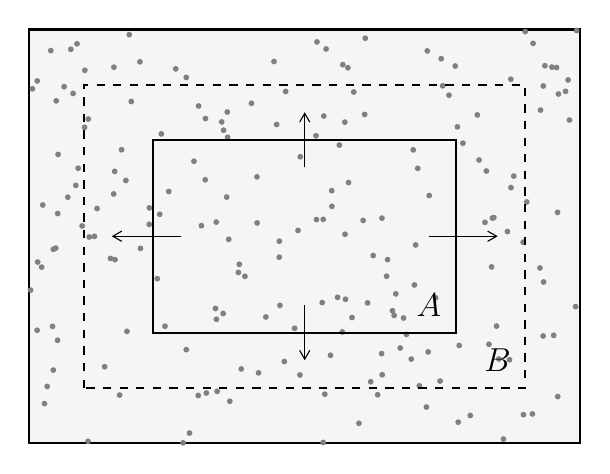
\begin{tikzpicture}[scale=0.35]
\fill[lightgray!15,draw=black,thick] (0,0) rectangle (20,15);

\fill[gray] (7.189873,12.007256) circle (3pt);
\fill[gray] (1.032745,3.725546) circle (3pt);
\fill[gray] (5.703827,13.261152) circle (3pt);
\fill[gray] (17.936429,1.025270) circle (3pt);
\fill[gray] (13.690591,3.939102) circle (3pt);
\fill[gray] (11.193998,5.283551) circle (3pt);
\fill[gray] (4.798022,11.213652) circle (3pt);
\fill[gray] (18.715176,13.688003) circle (3pt);
\fill[gray] (10.692704,11.860352) circle (3pt);
\fill[gray] (7.056115,11.346718) circle (3pt);
\fill[gray] (0.966585,7.071031) circle (3pt);
\fill[gray] (13.937926,10.633255) circle (3pt);
\fill[gray] (7.593829,6.185742) circle (3pt);
\fill[gray] (3.705931,12.388078) circle (3pt);
\fill[gray] (10.775614,14.295963) circle (3pt);
\fill[gray] (18.057741,8.744112) circle (3pt);
\fill[gray] (8.068603,12.323568) circle (3pt);
\fill[gray] (18.650144,3.881699) circle (3pt);
\fill[gray] (12.484510,6.800151) circle (3pt);
\fill[gray] (13.183608,4.794407) circle (3pt);
\fill[gray] (12.174938,11.920051) circle (3pt);
\fill[gray] (1.736886,14.482144) circle (3pt);
\fill[gray] (3.355545,10.638588) circle (3pt);
\fill[gray] (0.295411,13.134745) circle (3pt);
\fill[gray] (17.430353,3.016958) circle (3pt);
\fill[gray] (19.869400,14.962442) circle (3pt);
\fill[gray] (10.729442,1.767601) circle (3pt);
\fill[gray] (0.984080,12.412868) circle (3pt);
\fill[gray] (0.656211,2.050832) circle (3pt);
\fill[gray] (6.149162,12.226380) circle (3pt);
\fill[gray] (10.443128,14.550410) circle (3pt);
\fill[gray] (18.655995,12.951857) circle (3pt);
\fill[gray] (11.590530,9.448236) circle (3pt);
\fill[gray] (7.243261,7.388230) circle (3pt);
\fill[gray] (18.260829,1.052094) circle (3pt);
\fill[gray] (9.825389,2.467039) circle (3pt);
\fill[gray] (1.270561,12.927529) circle (3pt);
\fill[gray] (2.183670,7.471334) circle (3pt);
\fill[gray] (9.101712,4.988481) circle (3pt);
\fill[gray] (2.138719,0.055549) circle (3pt);
\fill[gray] (6.399133,11.770019) circle (3pt);
\fill[gray] (16.541260,8.003890) circle (3pt);
\fill[gray] (11.256169,10.807615) circle (3pt);
\fill[gray] (17.926257,7.283852) circle (3pt);
\fill[gray] (2.739774,2.765903) circle (3pt);
\fill[gray] (18.966992,13.637273) circle (3pt);
\fill[gray] (10.668147,0.016967) circle (3pt);
\fill[gray] (0.310205,6.564354) circle (3pt);
\fill[gray] (12.811328,2.473994) circle (3pt);
\fill[gray] (11.566809,13.614052) circle (3pt);
\fill[gray] (3.283881,1.735554) circle (3pt);
\fill[gray] (14.101612,9.963662) circle (3pt);
\fill[gray] (4.039885,7.059605) circle (3pt);
\fill[gray] (16.591664,9.866772) circle (3pt);
\fill[gray] (14.517395,8.977751) circle (3pt);
\fill[gray] (10.426222,8.104159) circle (3pt);
\fill[gray] (3.549166,4.048136) circle (3pt);
\fill[gray] (17.483642,9.263434) circle (3pt);
\fill[gray] (16.325371,10.266466) circle (3pt);
\fill[gray] (10.979845,9.152594) circle (3pt);
\fill[gray] (5.981012,10.220922) circle (3pt);
\fill[gray] (13.465983,3.443126) circle (3pt);
\fill[gray] (6.251647,7.884290) circle (3pt);
\fill[gray] (4.363000,8.528955) circle (3pt);
\fill[gray] (11.463047,7.570383) circle (3pt);
\fill[gray] (6.761937,4.878485) circle (3pt);
\fill[gray] (12.392466,2.219189) circle (3pt);
\fill[gray] (15.739529,10.876258) circle (3pt);
\fill[gray] (11.362909,4.028322) circle (3pt);
\fill[gray] (1.403271,8.917787) circle (3pt);
\fill[gray] (1.694522,9.344248) circle (3pt);
\fill[gray] (4.738868,8.295962) circle (3pt);
\fill[gray] (6.389808,9.547780) circle (3pt);
\fill[gray] (8.886094,13.840983) circle (3pt);
\fill[gray] (7.040599,4.696280) circle (3pt);
\fill[gray] (14.952140,13.942108) circle (3pt);
\fill[gray] (17.211416,0.139226) circle (3pt);
\fill[gray] (10.670952,8.112072) circle (3pt);
\fill[gray] (9.839079,10.382850) circle (3pt);
\fill[gray] (16.809571,8.160259) circle (3pt);
\fill[gray] (17.478862,13.197850) circle (3pt);
\fill[gray] (16.008395,0.995887) circle (3pt);
\fill[gray] (6.135184,1.721209) circle (3pt);
\fill[gray] (7.202958,11.088303) circle (3pt);
\fill[gray] (15.604905,3.537251) circle (3pt);
\fill[gray] (4.649788,5.960632) circle (3pt);
\fill[gray] (12.646831,1.748152) circle (3pt);
\fill[gray] (5.704931,3.385258) circle (3pt);
\fill[gray] (13.244499,4.627266) circle (3pt);
\fill[gray] (13.866541,3.042211) circle (3pt);
\fill[gray] (4.020821,13.829378) circle (3pt);
\fill[gray] (14.478915,3.303659) circle (3pt);
\fill[gray] (12.119582,8.071522) circle (3pt);
\fill[gray] (0.052974,5.544991) circle (3pt);
\fill[gray] (14.157844,2.072198) circle (3pt);
\fill[gray] (19.829076,4.945795) circle (3pt);
\fill[gray] (19.464476,12.758033) circle (3pt);
\fill[gray] (14.448449,14.224297) circle (3pt);
\fill[gray] (8.325068,2.544047) circle (3pt);
\fill[gray] (4.359520,7.930448) circle (3pt);
\fill[gray] (3.633524,14.815104) circle (3pt);
\fill[gray] (17.042602,3.044707) circle (3pt);
\fill[gray] (11.717216,4.551330) circle (3pt);
\fill[gray] (0.494682,8.633230) circle (3pt);
\fill[gray] (13.979299,5.732816) circle (3pt);
\fill[gray] (18.535276,6.350147) circle (3pt);
\fill[gray] (8.267637,9.654893) circle (3pt);
\fill[gray] (0.880287,7.026485) circle (3pt);
\fill[gray] (7.695881,2.684383) circle (3pt);
\fill[gray] (2.465090,8.505883) circle (3pt);
\fill[gray] (14.415714,1.302376) circle (3pt);
\fill[gray] (15.569702,0.753946) circle (3pt);
\fill[gray] (18.285254,14.497479) circle (3pt);
\fill[gray] (0.455887,6.378918) circle (3pt);
\fill[gray] (12.197111,14.685628) circle (3pt);
\fill[gray] (6.795592,4.486260) circle (3pt);
\fill[gray] (16.686419,3.579784) circle (3pt);
\fill[gray] (3.510219,9.522966) circle (3pt);
\fill[gray] (6.822231,1.872439) circle (3pt);
\fill[gray] (1.037286,8.323394) circle (3pt);
\fill[gray] (18.556981,12.076557) circle (3pt);
\fill[gray] (3.117391,6.651586) circle (3pt);
\fill[gray] (13.304852,5.408005) circle (3pt);
\fill[gray] (2.023153,13.521868) circle (3pt);
\fill[gray] (2.147448,11.752045) circle (3pt);
\fill[gray] (9.632847,4.159554) circle (3pt);
\fill[gray] (2.012655,11.451130) circle (3pt);
\fill[gray] (19.605825,11.716914) circle (3pt);
\fill[gray] (10.634260,5.094222) circle (3pt);
\fill[gray] (4.929862,4.234030) circle (3pt);
\fill[gray] (11.779346,12.733778) circle (3pt);
\fill[gray] (17.355771,7.671409) circle (3pt);
\fill[gray] (16.264088,11.902180) circle (3pt);
\fill[gray] (0.851292,4.229110) circle (3pt);
\fill[gray] (14.911070,2.246137) circle (3pt);
\fill[gray] (12.790055,3.240956) circle (3pt);
\fill[gray] (3.106337,9.853823) circle (3pt);
\fill[gray] (15.004812,12.957114) circle (3pt);
\fill[gray] (11.455350,11.640517) circle (3pt);
\fill[gray] (16.862233,8.176758) circle (3pt);
\fill[gray] (7.283005,1.511903) circle (3pt);
\fill[gray] (14.023672,7.183187) circle (3pt);
\fill[gray] (16.959859,4.239292) circle (3pt);
\fill[gray] (9.080443,7.321678) circle (3pt);
\fill[gray] (0.787920,14.235724) circle (3pt);
\fill[gray] (9.757357,7.711644) circle (3pt);
\fill[gray] (12.801919,8.156807) circle (3pt);
\fill[gray] (19.173654,8.365171) circle (3pt);
\fill[gray] (14.746939,5.266785) circle (3pt);
\fill[gray] (15.460890,13.675672) circle (3pt);
\fill[gray] (0.558498,1.426722) circle (3pt);
\fill[gray] (5.319326,13.573341) circle (3pt);
\fill[gray] (1.596066,12.682471) circle (3pt);
\fill[gray] (10.411521,11.148780) circle (3pt);
\fill[gray] (15.234786,12.617005) circle (3pt);
\fill[gray] (0.878152,2.643967) circle (3pt);
\fill[gray] (2.952409,6.694919) circle (3pt);
\fill[gray] (9.074063,6.740000) circle (3pt);
\fill[gray] (15.540580,11.468732) circle (3pt);
\fill[gray] (18.001669,14.926523) circle (3pt);
\fill[gray] (19.206391,12.660252) circle (3pt);
\fill[gray] (13.006573,6.651786) circle (3pt);
\fill[gray] (1.513548,14.283169) circle (3pt);
\fill[gray] (7.830906,6.044319) circle (3pt);
\fill[gray] (18.668757,5.840355) circle (3pt);
\fill[gray] (12.281253,5.082468) circle (3pt);
\fill[gray] (16.780682,6.387540) circle (3pt);
\fill[gray] (11.968683,0.711781) circle (3pt);
\fill[gray] (6.788235,8.014438) circle (3pt);
\fill[gray] (0.289549,4.087150) circle (3pt);
\fill[gray] (12.971851,6.048889) circle (3pt);
\fill[gray] (3.067813,9.033496) circle (3pt);
\fill[gray] (5.068369,9.124380) circle (3pt);
\fill[gray] (5.587748,0.003656) circle (3pt);
\fill[gray] (13.586570,4.533691) circle (3pt);
\fill[gray] (6.431809,1.813709) circle (3pt);
\fill[gray] (0.119261,12.849029) circle (3pt);
\fill[gray] (11.383318,13.725656) circle (3pt);
\fill[gray] (3.075973,13.633286) circle (3pt);
\fill[gray] (8.271872,7.982950) circle (3pt);
\fill[gray] (9.259674,2.953089) circle (3pt);
\fill[gray] (9.308203,12.753614) circle (3pt);
\fill[gray] (1.923948,7.874574) circle (3pt);
\fill[gray] (10.934866,3.180220) circle (3pt);
\fill[gray] (19.138825,13.620963) circle (3pt);
\fill[gray] (7.627648,6.481897) circle (3pt);
\fill[gray] (19.180860,1.683719) circle (3pt);
\fill[gray] (8.589508,4.571152) circle (3pt);
\fill[gray] (7.168202,8.919764) circle (3pt);
\fill[gray] (17.585780,9.683140) circle (3pt);
\fill[gray] (10.985187,8.586106) circle (3pt);
\fill[gray] (8.981215,11.553663) circle (3pt);
\fill[gray] (11.481412,5.212075) circle (3pt);
\fill[gray] (19.557651,13.170481) circle (3pt);
\fill[gray] (1.779307,9.969640) circle (3pt);
\fill[gray] (19.033129,3.905117) circle (3pt);
\fill[gray] (1.050651,10.469207) circle (3pt);
\fill[gray] (2.370389,7.496352) circle (3pt);
\fill[gray] (6.988479,11.647790) circle (3pt);
\fill[gray] (5.818615,0.357924) circle (3pt);

\draw[black,thick] (4.5,4) rectangle (15.5,11);
\draw[black,thick,dashed] (2,2) rectangle (18,13);
\draw[->,>=angle 60,black] (10,10) --(10,12);
\draw[->,>=angle 60,black] (10,5) --(10,3);
\draw[->,>=angle 60,black] (14.5,7.5) -- (17,7.5);
\draw[->,>=angle 60,black] (5.5,7.5) -- (3,7.5);
\node at (14.5,5) {\large $A$};
\node at (17,3) {\large $B$};

\end{tikzpicture}
\label{fig:zooming}
\end{figure}
	\begin{itemize}
		\item Give priority to already chosen centroids
	\end{itemize}
}

\frame{
	\frametitle{4. Future Work}
	\begin{itemize}
		\item Integration with the Web application.
		\item Further research on range search algorithms
		\item Experiment with different notions of representations.
	\end{itemize}	
	
}


\frame{
	
	}

\frame{
	\frametitle{Integer Linear Programming}
	\framesubtitle{$k$-centre}
	\begin{align*}
	\text{minimise}   \quad& D							   &\\
	\text{subject to} \quad
	& \sum\limits_{j=1}^{N}{y_j} = k 
	& 							\\
	& \sum\limits_{j=1}^{N}{x_{ij}}	= 1   
	& i=1,\ldots,N 				\\
	& \sum\limits_{j=1}^{N}{d_{ij} x_{ij}} \leq D
	& i=1,\ldots,N				\\
	& x_{ij} \leq y_{j}				   
	& i=1,\ldots,N;j=1,\ldots,N	\\
	& x_{ij},y_{j} \in \{0,1\}
	& i=1,\ldots,N;j=1,\ldots,N 
	\end{align*}
}


\frame{
	\frametitle{Integer Linear Programming}
	\framesubtitle{Geometric Disk Cover}
	\begin{align*}
		\text{minimise}   \quad& k							   &\\
		\text{subject to} \quad
		& \sum\limits_{j=1}^{N}{y_j} \leq k 
		& 							\\
		& \sum\limits_{j=1}^{N}{x_{ij}}	= 1   
		& i=1,\ldots,N 				\\
		& \sum\limits_{j=1}^{N}{d_{ij} x_{ij}} \leq D
		& i=1,\ldots,N				\\
		& x_{ij} \leq y_{j}				   
		& i=1,\ldots,N;j=1,\ldots,N	\\
		& x_{ij},y_{j} \in \{0,1\}
		& i=1,\ldots,N;j=1,\ldots,N 
	\end{align*}
}


\frame{
	\frametitle{Delaunay Triangulations}
	\begin{figure}[H]
	\begin{center}
		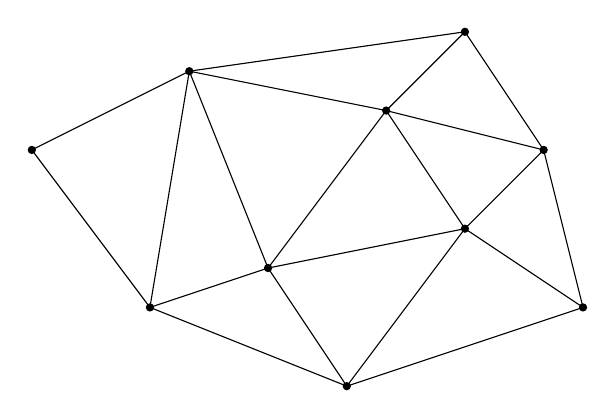
\begin{tikzpicture}[scale=0.5]
		%\draw [<->,thick] (0,10) node (yaxis) [left] {}
		%|- (15,0) node (xaxis) [below] {};
		%centroids
		\fill ( 2, 7) circle (3pt);
		\fill ( 5, 3) circle (3pt);
		\fill ( 6, 9) circle (3pt);
		\fill ( 8, 4) circle (3pt);
		\fill (10, 1) circle (3pt);
		\fill (11, 8) circle (3pt);
		\fill (13, 5) circle (3pt);
		\fill (13,10) circle (3pt);
		\fill (15, 7) circle (3pt);
		\fill (16, 3) circle (3pt);
		
		
		\draw [-] ( 2,7) -- ( 6,9);
		\draw [-] ( 6,9) -- ( 5,3);
		\draw [-] ( 5,3) -- ( 2,7);
		\draw [-] ( 6,9) -- ( 8,4);
		\draw [-] (10,1) -- ( 8,4);
		\draw [-] ( 5,3) -- (10,1);
		\draw [-] ( 8,4) -- ( 5,3);
		\draw [-] ( 8,4) -- (11,8);
		\draw [-] (11,8) -- (6,9);
		\draw [-] ( 6,9) -- (13,10);
		\draw [-] (11,8) -- (13,10);
		\draw [-] (15,7) -- (13,10);
		\draw [-] (16,3) -- (15,7);
		\draw [-] (16,3) -- (10,1);
		\draw [-] (16,3) -- (13,5);
		\draw [-] (13,5) -- (15,7);
		\draw [-] (13,5) -- (10,1);
		\draw [-] (13,5) -- (8,4);
		\draw [-] (13,5) -- (11,8);
		\draw [-] (15,7) -- (11,8);
		\end{tikzpicture}
	\end{center}
\end{figure}
}

\frame{
	\frametitle{Delaunay Triangulations}
	\begin{figure}[H]
	\begin{center}
		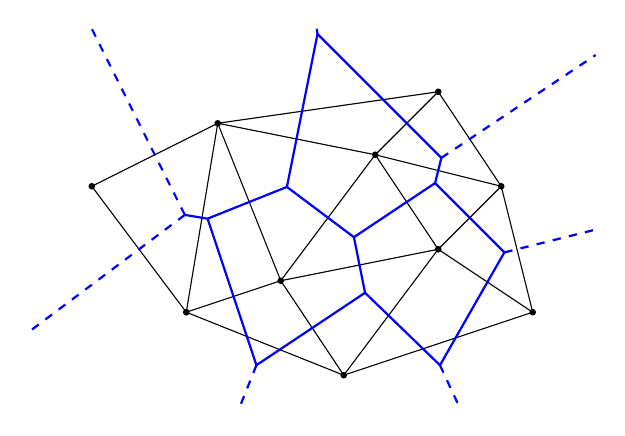
\begin{tikzpicture}[scale=0.4]
		%\draw [<->,thick] (0,10) node (yaxis) [left] {}
		%|- (15,0) node (xaxis) [below] {};
		%centroids
		\fill ( 2, 7) circle (3pt);
		\fill ( 5, 3) circle (3pt);
		\fill ( 6, 9) circle (3pt);
		\fill ( 8, 4) circle (3pt);
		\fill (10, 1) circle (3pt);
		\fill (11, 8) circle (3pt);
		\fill (13, 5) circle (3pt);
		\fill (13,10) circle (3pt);
		\fill (15, 7) circle (3pt);
		\fill (16, 3) circle (3pt);
		
		%DELAUNAY
		\draw [-] ( 2,7) -- ( 6,9);
		\draw [-] ( 6,9) -- ( 5,3);
		\draw [-] ( 5,3) -- ( 2,7);
		\draw [-] ( 6,9) -- ( 8,4);
		\draw [-] (10,1) -- ( 8,4);
		\draw [-] ( 5,3) -- (10,1);
		\draw [-] ( 8,4) -- ( 5,3);
		\draw [-] ( 8,4) -- (11,8);
		\draw [-] (11,8) -- (6,9);
		\draw [-] ( 6,9) -- (13,10);
		\draw [-] (11,8) -- (13,10);
		\draw [-] (15,7) -- (13,10);
		\draw [-] (16,3) -- (15,7);
		\draw [-] (16,3) -- (10,1);
		\draw [-] (16,3) -- (13,5);
		\draw [-] (13,5) -- (15,7);
		\draw [-] (13,5) -- (10,1);
		\draw [-] (13,5) -- (8,4);
		\draw [-] (13,5) -- (11,8);
		\draw [-] (15,7) -- (11,8);
		
		%VORONOI		
		\draw [-,blue,thick] ( 5.6764, 5.9706) -- ( 4.9545, 6.0909);
		\draw [-,blue,thick] ( 5.6764, 5.9706) -- ( 8.1956, 6.9783);
		\draw [-,blue,thick] (10.3235, 5.3824) -- ( 8.1956, 6.9783);
		\draw [-,blue,thick] (10.3235, 5.3824) -- (10.6765, 3.6176);
		\draw [-,blue,thick] ( 7.2272, 1.3182) -- (10.6765, 3.6176);
		\draw [-,blue,thick] ( 7.2272, 1.3182) -- ( 5.6764, 5.9706);
		\draw [-,blue,thick] (13.0556, 1.3182) -- (10.6765, 3.6176);
		\draw [-,blue,thick] (13.0556, 1.3182) -- (15.1000, 4.9000);
		\draw [-,blue,thick] (12.9000, 7.1000) -- (15.1000, 4.9000);
		\draw [-,blue,thick] (12.9000, 7.1000) -- (10.3235, 5.3824);
		\draw [-,blue,thick] (12.9000, 7.1000) -- (13.1000, 7.9000);
		\draw [-,blue,thick] ( 9.1667,11.8333) -- (13.1000, 7.9000);
		\draw [-,blue,thick] ( 9.1667,11.8333) -- ( 8.1956, 6.9783);
		
		\draw [-,blue,thick,dashed] ( 4.9545, 6.0909) -- (	2.0000,12.0000);
		\draw [-,blue,thick,dashed] ( 4.9545, 6.0909) -- (	0.0000,	2.3750);
		\draw [-,blue,thick,dashed] ( 7.2272, 1.3182) -- (	6.7000, 0.0000);
		\draw [-,blue,thick,dashed] (13.0556, 1.3182) -- (13.6667, 0.0000);
		\draw [-,blue,thick,dashed] (15.1000, 4.9000) -- (18.0000, 5.6250);
		\draw [-,blue,thick,dashed] (13.1000, 7.9000) -- (18.0000,11.1667);
		\draw [-,blue,thick,dashed] ( 9.1667,11.8333) -- ( 9.1429,12.0000);
		
		\end{tikzpicture}
	\end{center}
	\caption{Overlap of a Voronoi Diagram and its Delaunay Triangulation}
	\label{fig:dt_vd}
\end{figure}
}

\frame{
	\frametitle{Voronoi Diagrams}
	\begin{figure}[!h]
	\begin{center}
		\begin{tikzpicture}[scale=0.4]
		%\draw [<->,thick] (0,10) node (yaxis) [left] {}
		%|- (15,0) node (xaxis) [below] {};
		%centroids
		\fill ( 2, 7) circle (3pt);
		\fill ( 5, 3) circle (3pt);
		\fill ( 6, 9) circle (3pt);
		\fill ( 8, 4) circle (3pt);
		\fill (10, 1) circle (3pt);
		\fill (11, 8) circle (3pt);
		\fill (13, 5) circle (3pt);
		\fill (13,10) circle (3pt);
		\fill (15, 7) circle (3pt);
		\fill (16, 3) circle (3pt);
		
		\draw [-] ( 5.6764, 5.9706) -- ( 4.9545, 6.0909);
		\draw [-] ( 5.6764, 5.9706) -- ( 8.1956, 6.9783);
		\draw [-] (10.3235, 5.3824) -- ( 8.1956, 6.9783);
		\draw [-] (10.3235, 5.3824) -- (10.6765, 3.6176);
		\draw [-] ( 7.2272, 1.3182) -- (10.6765, 3.6176);
		\draw [-] ( 7.2272, 1.3182) -- ( 5.6764, 5.9706);
		\draw [-] (13.0556, 1.3182) -- (10.6765, 3.6176);
		\draw [-] (13.0556, 1.3182) -- (15.1000, 4.9000);
		\draw [-] (12.9000, 7.1000) -- (15.1000, 4.9000);
		\draw [-] (12.9000, 7.1000) -- (10.3235, 5.3824);
		\draw [-] (12.9000, 7.1000) -- (13.1000, 7.9000);
		\draw [-] ( 9.1667,11.8333) -- (13.1000, 7.9000);
		\draw [-] ( 9.1667,11.8333) -- ( 8.1956, 6.9783);

		\draw [-,dashed] ( 4.9545, 6.0909) -- (2 , 12);
		\draw [-,dashed] ( 4.9545, 6.0909) -- (0, 2.375);
		\draw [-,dashed] ( 7.2272, 1.3182) -- ( 6.7, 0);
		\draw [-,dashed] (13.0556, 1.3182) -- (13.6667, 0);
		\draw [-,dashed] (15.1000, 4.9000) -- (18, 5.625);
		\draw [-,dashed] (13.1000, 7.9000) -- (18, 11.1667);
		\draw [-,dashed] ( 9.1667,11.8333) -- ( 9.1429, 12);
		
		\end{tikzpicture}
	\end{center}
	\caption{Example of a Voronoi Diagram}
	\label{fig:vd1}
\end{figure}
}

\frame{
	\frametitle{Greedy Routing}
	\begin{figure}[H]
	\begin{center}
		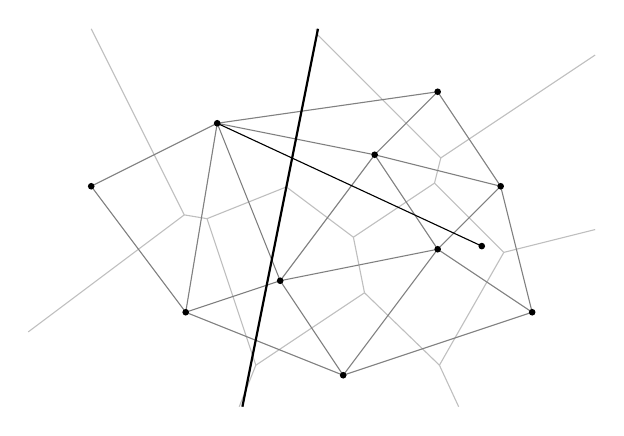
\begin{tikzpicture}[scale=0.4]
		%\draw [<->,thick] (0,10) node (yaxis) [left] {}
		%|- (15,0) node (xaxis) [below] {};
		
		%VORONOI
		\draw [-,gray!50] ( 5.6764, 5.9706) -- ( 4.9545, 6.0909);
		\draw [-,gray!50] ( 5.6764, 5.9706) -- ( 8.1956, 6.9783);
		\draw [-,gray!50] (10.3235, 5.3824) -- ( 8.1956, 6.9783);
		\draw [-,gray!50] (10.3235, 5.3824) -- (10.6765, 3.6176);
		\draw [-,gray!50] ( 7.2272, 1.3182) -- (10.6765, 3.6176);
		\draw [-,gray!50] ( 7.2272, 1.3182) -- ( 5.6764, 5.9706);
		\draw [-,gray!50] (13.0556, 1.3182) -- (10.6765, 3.6176);
		\draw [-,gray!50] (13.0556, 1.3182) -- (15.1000, 4.9000);
		\draw [-,gray!50] (12.9000, 7.1000) -- (15.1000, 4.9000);
		\draw [-,gray!50] (12.9000, 7.1000) -- (10.3235, 5.3824);
		\draw [-,gray!50] (12.9000, 7.1000) -- (13.1000, 7.9000);
		\draw [-,gray!50] ( 9.1667,11.8333) -- (13.1000, 7.9000);
		%\draw [-,gray!50] ( 9.1667,11.8333) -- ( 8.1956, 6.9783);
		%VORONOI EXTENDED
		\draw [-,gray!50] ( 4.9545, 6.0909) -- (2 , 12);
		\draw [-,gray!50] ( 4.9545, 6.0909) -- (0, 2.375);
		\draw [-,gray!50] ( 7.2272, 1.3182) -- ( 6.7, 0);
		\draw [-,gray!50] (13.0556, 1.3182) -- (13.6667, 0);
		\draw [-,gray!50] (15.1000, 4.9000) -- (18, 5.625);
		\draw [-,gray!50] (13.1000, 7.9000) -- (18, 11.1667);
		\draw [-,gray!50] ( 9.1667,11.8333) -- ( 9.1429, 12);
		
		%DELAUNAY
		\draw [-,gray] ( 2,7) -- ( 6,9);
		\draw [-,gray] ( 6,9) -- ( 5,3);
		\draw [-,gray] ( 5,3) -- ( 2,7);
		\draw [-,gray] ( 6,9) -- ( 8,4);
		\draw [-,gray] (10,1) -- ( 8,4);
		\draw [-,gray] ( 5,3) -- (10,1);
		\draw [-,gray] ( 8,4) -- ( 5,3);
		\draw [-,gray] ( 8,4) -- (11,8);
		\draw [-,gray] (11,8) -- (6,9);
		\draw [-,gray] ( 6,9) -- (13,10);
		\draw [-,gray] (11,8) -- (13,10);
		\draw [-,gray] (15,7) -- (13,10);
		\draw [-,gray] (16,3) -- (15,7);
		\draw [-,gray] (16,3) -- (10,1);
		\draw [-,gray] (16,3) -- (13,5);
		\draw [-,gray] (13,5) -- (15,7);
		\draw [-,gray] (13,5) -- (10,1);
		\draw [-,gray] (13,5) -- (8,4);
		\draw [-,gray] (13,5) -- (11,8);
		\draw [-,gray] (15,7) -- (11,8);
		
		
		%POINTS
		
		\fill ( 2, 7) circle (3pt);
		\fill ( 5, 3) circle (3pt);
		\fill ( 6, 9) circle (3pt);
		\fill ( 8, 4) circle (3pt);
		\fill (10, 1) circle (3pt);
		\fill (11, 8) circle (3pt);
		\fill (13, 5) circle (3pt);
		\fill (13,10) circle (3pt);
		\fill (15, 7) circle (3pt);
		\fill (16, 3) circle (3pt);
		
		%EDGE E
		\draw [-,thick] ( 6.8,0) -- ( 9.2, 12);
		\draw [-]( 6,9) -- ( 14.4, 5.1);
		\fill (14.4, 5.1) circle (3pt);
		
		\end{tikzpicture}
	\end{center}
	\caption{Example of the Greedy Routing Algorithm}
	\label{fig:gr1}
\end{figure}
}

\frame{
	\frametitle{$k$-d Trees}
	\input{Figures/kd1}
}

\frame{
	\frametitle{$k$-d Trees Range Search}
	\begin{figure}[H]
	\begin{center}
		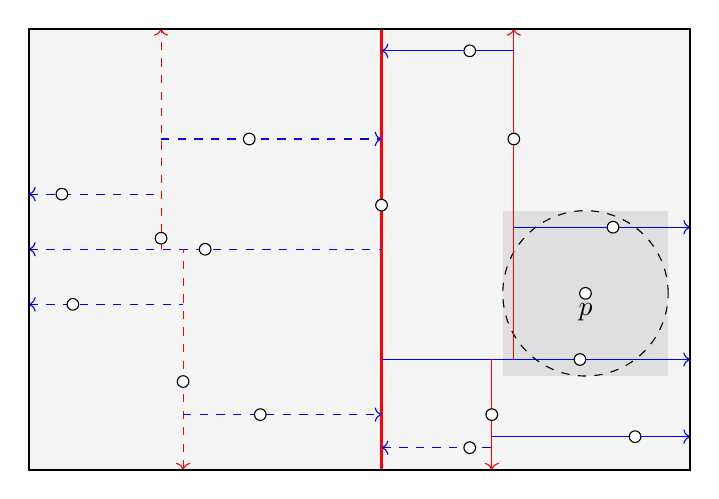
\begin{tikzpicture}[scale=1.4]
		\fill[lightgray!15] (0,0) rectangle (6,4);
		\fill[lightgray!50] (4.3,0.85) rectangle (5.8,2.35);
		\draw[dashed](5.05,1.6) circle(0.75);
		\fill[white,draw=black] (5.05,1.6) circle(1.5pt);
		\node[below] at (5.05,1.6) {$\tiny p$};
		
		\draw [red,thick](3.2,0) -- (3.2,4);
		\fill[white,draw=black] (3.2,2.4) circle (1.5pt);
		\draw [blue,->](3.2,1) -- (6,1);
		\fill[white,draw=black] (5,1) circle (1.5pt);
		\draw [red,<-](4.2,0) -- (4.2,1);
		\fill[white,draw=black] (4.2,0.5) circle (1.5pt);
		\draw [blue,<-,dashed](3.2,0.2) -- (4.2,0.2);
		\fill[white,draw=black] (4,0.2) circle (1.5pt);
		\draw [blue,->](4.2,0.3) -- (6,0.3);
		\fill[white,draw=black] (5.5,0.3) circle (1.5pt);
		\draw [red,->](4.4,1) -- (4.4,4);
		\fill[white,draw=black] (4.4,3) circle (1.5pt);
		\draw [blue,<-](3.2,3.8) -- (4.4,3.8);
		\fill[white,draw=black] (4,3.8) circle (1.5pt);
		\draw [blue,->](4.4,2.2) -- (6,2.2);
		\fill[white,draw=black] (5.3,2.2) circle (1.5pt);
		\draw [blue,<-,dashed](0,2) -- (3.2,2);
		\fill[white,draw=black] (1.6,2) circle (1.5pt);
		\draw [red,->,dashed](1.2,2) -- (1.2,4);
		\fill[white,draw=black] (1.2,2.1) circle (1.5pt);
		\draw [blue,->,dashed](1.2,3) -- (3.2,3);
		\fill[white,draw=black] (2,3) circle (1.5pt);
		\draw [blue,<-,dashed](0,2.5) -- (1.2,2.5);
		\fill[white,draw=black] (0.3,2.5) circle (1.5pt);
		\draw [red,<-,dashed](1.4,0) -- (1.4,2);
		\fill[white,draw=black] (1.4,0.8) circle (1.5pt);
		\draw [blue,->,dashed](1.4,0.5) -- (3.2,0.5);
		\fill[white,draw=black] (2.1,0.5) circle (1.5pt);
		\draw [blue,<-,dashed](0,1.5) -- (1.4,1.5);
		\fill[white,draw=black] (0.4,1.5) circle (1.5pt);
		\draw[thick] (0,0) rectangle (6,4);
		\end{tikzpicture}
	\end{center}
	\caption[Example of a range search query on a \kdTree] {The dashed lines are never queried, since the rectangle does not intercept their parent. This query searches for all points within a fixed distance of $p$.}
	\label{fig:kdrs}
\end{figure}
}

\frame{
	\frametitle{Line Sweep}
	\begin{figure}[H]
\begin{center}
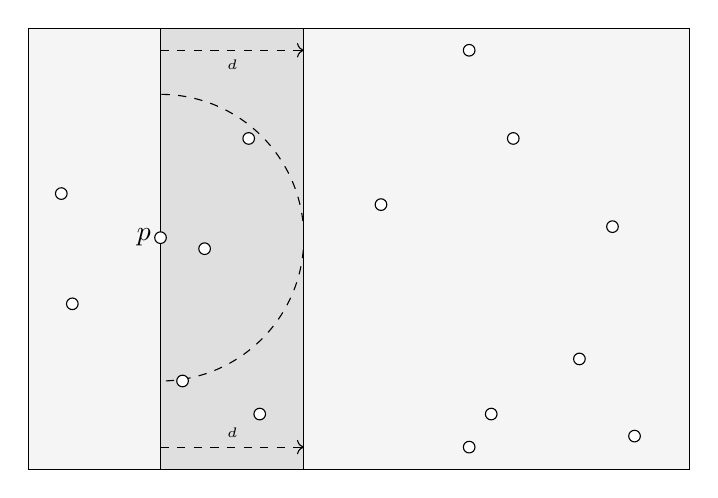
\begin{tikzpicture}[scale=1.4]
	\fill[lightgray!15,draw=black] (0,0) rectangle (6,4);
	\fill[lightgray!50,draw=black] (1.2,0) rectangle (2.5,4);
	\begin{scope}
	\clip (1.2,0) rectangle (2.5,4);
	\draw[dashed](1.2,2.1) circle (1.3);
	\end{scope}
	
	\draw [dashed,->](1.2,0.2) -- node[above]{\tiny$d$}(2.5,0.2);

	\draw [dashed,->](1.2,3.8) -- node[below]{\tiny$d$}(2.5,3.8);

	\node[left] at (1.2,2.1) {$\tiny p$};

	\fill[white,draw=black] (3.2,2.4) circle (1.5pt);
	\fill[white,draw=black] (5,1) circle (1.5pt);		
	\fill[white,draw=black] (4.2,0.5) circle (1.5pt);
	\fill[white,draw=black] (4,0.2) circle (1.5pt);
	\fill[white,draw=black] (5.5,0.3) circle (1.5pt);
	\fill[white,draw=black] (4.4,3) circle (1.5pt);
	\fill[white,draw=black] (4,3.8) circle (1.5pt);
	\fill[white,draw=black] (5.3,2.2) circle (1.5pt);
	\fill[white,draw=black] (1.6,2) circle (1.5pt);
	\fill[white,draw=black] (1.2,2.1) circle (1.5pt);
	\fill[white,draw=black] (2,3) circle (1.5pt);
	\fill[white,draw=black] (0.3,2.5) circle (1.5pt);
	\fill[white,draw=black] (1.4,0.8) circle (1.5pt);
	\fill[white,draw=black] (2.1,0.5) circle (1.5pt);
	\fill[white,draw=black] (0.4,1.5) circle (1.5pt);

\end{tikzpicture}
\end{center}
\caption[Illustration of the Line Sweep method.]{Illustration of the Line Sweep method. This query searches for the points within a given distance of $p$ that are to the right of $p$}
\label{fig:ls1}
\end{figure}
}

\frame{
	\frametitle{Geometric Disk Cover}
	\framesubtitle{Random Sampling}
	\begin{figure}[!h] 
	\vspace{-25pt}
	\centering
	\includegraphics[width=\linewidth]{Pictures/ls_rs_t} 
	\label{fig:ls_rs_t} 
\end{figure}
	\begin{itemize}
		\item Faster Times than the line sweep algorithm
	\end{itemize}
}
	
\frame{
	\frametitle{Geometric Disk Cover}
	\framesubtitle{Random Sampling}
	\begin{figure}[!h] 
	\vspace{-10pt}
	\centering
	\includegraphics[width=\linewidth]{Pictures/ls_rs_s} 
	\label{fig:ls_rs_s} 
\end{figure}
	\begin{itemize}
		\item Uses less memory (150Mb)
		\end{itemize}
}

\frame{
	\frametitle{Geometric Disk Cover}
	\framesubtitle{Random Sampling}
	\begin{figure}[!h] 
	\vspace{-10pt}
	\centering
	\includegraphics[width=\linewidth]{Pictures/ls_rs_k} 
	\caption[Number $k$ of points selected for Line Sweep and Random Sampling algorithms.]{Number $k$ of points selected for the line sweep algorithm, and two instances of the random sampling, which sample 5\% and 10\% of the number points, for different values of $d$.}
	\label{fig:ls_rs_k} 
\end{figure}
}


\end{document}